
\documentclass[]{report}\usepackage[]{graphicx}\usepackage[]{color}
%% maxwidth is the original width if it is less than linewidth
%% otherwise use linewidth (to make sure the graphics do not exceed the margin)
\makeatletter
\def\maxwidth{ %
  \ifdim\Gin@nat@width>\linewidth
    \linewidth
  \else
    \Gin@nat@width
  \fi
}
\makeatother

\definecolor{fgcolor}{rgb}{0.345, 0.345, 0.345}
\newcommand{\hlnum}[1]{\textcolor[rgb]{0.686,0.059,0.569}{#1}}%
\newcommand{\hlstr}[1]{\textcolor[rgb]{0.192,0.494,0.8}{#1}}%
\newcommand{\hlcom}[1]{\textcolor[rgb]{0.678,0.584,0.686}{\textit{#1}}}%
\newcommand{\hlopt}[1]{\textcolor[rgb]{0,0,0}{#1}}%
\newcommand{\hlstd}[1]{\textcolor[rgb]{0.345,0.345,0.345}{#1}}%
\newcommand{\hlkwa}[1]{\textcolor[rgb]{0.161,0.373,0.58}{\textbf{#1}}}%
\newcommand{\hlkwb}[1]{\textcolor[rgb]{0.69,0.353,0.396}{#1}}%
\newcommand{\hlkwc}[1]{\textcolor[rgb]{0.333,0.667,0.333}{#1}}%
\newcommand{\hlkwd}[1]{\textcolor[rgb]{0.737,0.353,0.396}{\textbf{#1}}}%
\let\hlipl\hlkwb

\usepackage{framed}
\makeatletter
\newenvironment{kframe}{%
 \def\at@end@of@kframe{}%
 \ifinner\ifhmode%
  \def\at@end@of@kframe{\end{minipage}}%
  \begin{minipage}{\columnwidth}%
 \fi\fi%
 \def\FrameCommand##1{\hskip\@totalleftmargin \hskip-\fboxsep
 \colorbox{shadecolor}{##1}\hskip-\fboxsep
     % There is no \\@totalrightmargin, so:
     \hskip-\linewidth \hskip-\@totalleftmargin \hskip\columnwidth}%
 \MakeFramed {\advance\hsize-\width
   \@totalleftmargin\z@ \linewidth\hsize
   \@setminipage}}%
 {\par\unskip\endMakeFramed%
 \at@end@of@kframe}
\makeatother

\definecolor{shadecolor}{rgb}{.97, .97, .97}
\definecolor{messagecolor}{rgb}{0, 0, 0}
\definecolor{warningcolor}{rgb}{1, 0, 1}
\definecolor{errorcolor}{rgb}{1, 0, 0}
\newenvironment{knitrout}{}{} % an empty environment to be redefined in TeX

\usepackage{alltt}
\usepackage[english]{babel}
\usepackage{graphicx}





% Title Page
\title{Analyzing data using linear models}

\author{St\'ephanie van den Berg}
\date{Versie 0.1 \\ (\today)}
\IfFileExists{upquote.sty}{\usepackage{upquote}}{}
\begin{document}
\maketitle




\begin{abstract}
This book is intended to be of use to bachelor students in social sciences that want to learn how to analyze their data, with the specific aim to answer research questions. The book has a practical take on data analysis: how to do it, how to interpret the results, and how to report the results. All techniques are presented within the framework of linear models: this includes simple regression models, to linear mixed models, and generalized linear models. All methods can be carried out within one supermodel: the generalized linear mixed model. This approach is illustrated using SPSS.
\end{abstract}


\tableofcontents


% % knit_child('chapter_1.Rnw') % exploring your data, descriptive statistics
% % 
% % \chapter{Linear modelling: introduction FULYA}
% % \section{Linear relationships}
% % \section{Pearson correlation}
% % \section{Simple regression with a continuous predictor}
% % \section{Predicting the dependent variable}
% % 
% % 
% % 



\chapter{Multivariate regression}


\section{Explained and unexplained variance}

In the previous chapter we have seen relationships between two variables: one dependent variable and one independent variable. The dependent variable we usually denote as $y$, and the indepedent variable we denote by $x$. The relationship was modelled by a linear equation: an equation with an intercept $b_0$ and a slope parameter $b_1$:


\begin{equation}
y = b_0 + b_1 x
\end{equation}

Further, we argued that in most cases, the relationship between $x$ and $y$ cannot be completely described by a straight line. Not all of the variation in $y$ can be explained by the variation in $x$. Therefore, we have \textit{residuals} $e$: the difference between the $y$-values that are predicted by the straight line, (denoted by $\hat{y}$), and the observed $y$-value:

\begin{equation}
e = \hat{y} - y
\end{equation}

Therefore, the relationship between $x$ and $y$ is denoted by a regression equation, where the relationship is approached by a linear equation, plus a residual part $e$:

\begin{equation}
y = b_0 + b_1 x + e
\end{equation}

The linear equation only gives us only the expected $y$-value, $\hat{y}$:


\begin{equation}
\hat{y} = b_0 + b_1 x
\end{equation}


We've also seen that the residual $e$ is assumed to have a normal distribution, with mean 0 and variance $\sigma^2$:


\begin{equation}
e \sim N(0,\sigma^2)
\end{equation}

Remember that linear models are used to explain (or predict) the variation in $y$: why are there both high values of $y$ and some low values? Where does the variance in $y$ come from? Well, the linear model tells us that the variation is in part explained by the variation in $x$. If $b_1$ is positive, we predict a relatively high value for $y$ for a high value of $x$, and we predict a relatively low value for $y$ if we have a low value for $x$. If $b_1$ is negative, it is of course in the opposite direction. Thus, the variance in $y$ is in part explained by the variance in $x$, and the rest of the variance can only be explained by the residuals $e$.



\begin{equation}
Var(y) = Var(\hat{y}) + Var(e) = Var(b_0 + b_1 x) + \sigma^2
\end{equation}


Because the residuals do not explain anything (we don't know where these residuals come from), we say that the \textit{explained} variance of $y$ is only that part of the variance that is explained by independent variable $x$: $Var(b_0 + b_1 x)$. The \textit{unexplained} variance of $y$ is the variance of the residuals, $\sigma^2$. The explained variance is often denoted by a ratio: the explained variance divided by the total variance of $y$:


\begin{equation}
Var_{explained} = \frac{Var(b_0+b_1 x)}{Var(y)} = \frac{Var(b_0+b_1 x)}{Var(b_0+b_1 x) + \sigma^2}
\end{equation}

From this equation we see that if the variance of the residuals is large, then the explained variance is small. If the variance of the residuals is small, the variance explained is large.


\section{More than one predictor}

In regression analysis, and in linear models in general, we try to make the explained variance as large as possible. In other words, we try to minimize the residual variance, $\sigma^2$.

One way to do that is to use a second independent variable. If not all of the variance in $y$ is explained by $x$, then why not try an extra independent variable?


Let's use an example with data on the weight of books, the size of books (area), and the volume of books. Let's try first to predict the weight of a book, $weight$, on the basis of the volume of the book, $volume$. Suppose we find the following regression equation and a value for $\sigma^2$:






\begin{eqnarray}
weight = 107.7 + 0.71 \times  volume + e \\
e \sim N(0, 15362)
\end{eqnarray}


In the data set, we see that the variance of the weight, $Var(weight)$ is equal to 72274. Since we also know the variance of the residuals, we can solve for the variance explained by \textbf{volume}:


\begin{eqnarray}
Var(weight) =  72274=   Var(107.7 + 0.7 \times  volume) + 15362 \nonumber\\
Var(107.7 + 0.7 \times  volume) = 72274- 15362= 56912\nonumber
\end{eqnarray}

So the proportion of explained variance is equal to $ \frac{56912}{72274}=0.7874478$. This is quite a high proportion: nearly all of the variation in the number of houses per city is explained by how many inhabitants a city has.
\\
\\
But let's see if we can explain even more variance if we add an extra independent variable. Suppose we know the area of each book. We expect that books with a large area weigh more. Our linear equation might look like this:


\begin{eqnarray}
weight = 22.4 + 0.71 \times volume + 0.5 \times  area + e \\
e \sim N(0, 6031)
\end{eqnarray}

How much of the variance in weight does this equation explain? The proportion of explained variance is equal to $ \frac{66243}{72274}=0.9165537$. So the proportion of explained variance has increased!

Note that the variance of the residuals has decreased; this is the main reason why the proportion of explained variance has increased. By adding the extra independent variable, we can explain some of the variance that without this variable could not be explained! In summary, by adding independent variables to a regression equation, we can explain more of the variance of the dependent variable. A regression analysis with more than one independent variable we call \textit{multiple regression}. Regression with only one indendent variable is often called \textit{simple regression}.







\section{R-squared}

With regression analysis, we try to explain variance of the dependent variable. With multiple regression, we use more than one independent variable to try to explain this variance. In regression analysis, we use the term R-squared to refer to the proportion of explained variance, usually with the symbol $R^2$. The unexplained variance is of course the variance of the residuals, $Var(e)$, usually denoted as $\sigma_e^2$. So suppose the variance of dependent variable $y$ equals 100, and the residual variance in a regression equation equals say 80, then $R^2$ or the proportion of explained variance is $(100-80)/100=0.20$.

\begin{eqnarray}
R^2 = \sigma^2_{explained}/ \sigma^2_y = (1-\sigma^2_{unexplained})/\sigma^2_y = (1-\sigma^2_e)/\sigma^2_y
\end{eqnarray}

This is the defintion of R-squared at the population level, where we know the exact values of the variances. However, regression analysis is most often based on a random sample of the population, and we don't know the values exactly, we can only try to estimate them.

For $\sigma_y^2$ we take as an adjusted estimate the variance of $y$ in our sample data, Var($y$), which is calculated by


\begin{eqnarray}
\widehat{\sigma_y^2} =  \frac{  \Sigma (y-\bar{y})^2  }{n-1}
\end{eqnarray}

where $n$ is sample size. We divide by $n-1$ and not by $n$, because we want to estimate the variance of $y$ in the population data.

For $\sigma_e^2$ we take as an adjusted estimate the variance of the residuals $e$ in our sample data, Var($e$), which is calculated by


\begin{eqnarray}
\widehat{\sigma_e^2} =  \frac{  \Sigma e^2  }{n-1}
\end{eqnarray}

Here we do not have to subtract the mean of the residuals, because this is 0 by definition.

So our estimate for $R^2$ in the population is then


\begin{eqnarray}
\widehat{R^2} &=&  \frac   { \frac{  \Sigma (y-\bar{y})^2  }{n-1}- \frac{  \Sigma e^2  }{n-1}}{\frac{  \Sigma (y-\bar{y})^2  }{n-1}} \nonumber\\
&=& \frac{ \Sigma (y-\bar{y})^2 - \Sigma e^2}{\Sigma (y-\bar{y})^2} = 1 - \frac{SSE}{SST}
\end{eqnarray}

where SST refers to the total sum of squares.

As we saw previously, in a regression analysis, the intercept and slope parameters are found by minimizing the sum of squares of the residuals, $SSE$. Since the variance of the residuals is based on this sum of squares, in any regression analysis, the variance of the residuals is always as small as possible. The values of the parameters for which the $SSE$ (and by consequence the variance) is smallest, are the least squares regression parameters. And if the variance of the residuals is always minimized in a regression analysis, the explained variance is always maximized!

Because in any least squares regression analysis based on a sample of data, the explained variance is always maximized, we may overestimate the variance explained in the population data. Therefore very often in regression analysis we use an \textit{adjusted R-squared} that takes this possible overestimation (\textit{inflation}) into account. The adjustment is based on the number of independent variables and sample size.

The formula is


\begin{eqnarray}
R^2_{adj}= 1 - (1-R^2)\frac{n-1}{n-p-1} \nonumber
\end{eqnarray}

where $n$ is sample size and $p$ is the number of independent variables. For example, if $R^2$ equals 0.10 and we have a sample size of 100 and 2 independent variables, the adjusted $R^2$ is equal to $1 - (1-0.10)\frac{100-1}{100-2-1}= 1 - (0.90)\frac{99}{97}=0.08$. Thus the estimated proportion of variance explained at population level equals 0.08. Remember that the adjusted R-squared is \textit{never larger} than the unadjusted R-squared.




\section{Multicollinearity}

In general, if you add independent variables to a regression equation, the proportion explained variance, $R^2$, increases. Suppose you have the following three regression equations:

\begin{eqnarray}
weight = b_0 + b_1 \times  volume + e \\
weight = b_0 + b_1 \times  area + e \\
weight = b_0 + b_1 \times  volume + b_1 \times  area + e
\end{eqnarray}

If we carry out these three analyses, we obtain an $R^2$ of 0.8026346 if we only use \textbf{volume} as predictor, and an $R^2$ of 0.1268163 if we only use \textbf{area} as predictor. So perhaps you'd think that if we take both \textbf{volume} and \textbf{area} as predictors in the model, we would get an $R^2$ of $0.8026346+0.1268163= 0.9294509$. However, if we carry out the multiple regression with \textbf{volume} and \textbf{area}, we obtain an $R^2$ of 0.9284738, which is slightly less! This is not a rounding error, but the result of the fact that there is a correlation between the volume of a book and the area of a book. Here it is a tiny correlation of $round(cor(allbacks$area, allbacks$volume),3)$, but nevertheless it affects the proportion of variance explained when you use both these variables.


Let's look at what happens when indendent variables are strongly correlated. Table \ref{tab:multi_2} shows measurements on a breed of seals (only measurements on the first 6 seals are shown). Often, the age of an animal is gaged from its weight: we assume that heavier seals are older than lighter seals. If we carry out a simple regression analysis, we get the following equation:


% latex table generated in R 3.4.2 by xtable 1.8-2 package
% Fri May  4 10:40:27 2018
\begin{table}[ht]
\centering
\caption{Part of Cape Fur Seal Data.} 
\label{tab:multi_2}
\begin{tabular}{rrr}
  \hline
age & weight & heart \\ 
  \hline
33.00 & 27.50 & 127.70 \\ 
  10.00 & 24.30 & 93.20 \\ 
  10.00 & 22.00 & 84.50 \\ 
  10.00 & 18.50 & 85.40 \\ 
  12.00 & 28.00 & 182.00 \\ 
  18.00 & 23.80 & 130.00 \\ 
   \hline
\end{tabular}
\end{table}



\begin{eqnarray}
age = 11.4 + 0.82 \times  weight + e \\
e \sim N(0, 200)
\end{eqnarray}


USE regression table instead of formula




From the data we calculate the variance of age, and we find that it is 1090.8551724. The variance of the residuals is 200, so that the proportion of explained variance is $(1090.8551724-200)/1090.8551724  = 0.8166576$.

Since we also have data on the weight of the heart alone, we could try to predict the age from the weight of the heart. Then we get:


\begin{eqnarray}
age = 20.6 + 0.11 \times  heart + e \\
e \sim N(0, 307)
\end{eqnarray}

USE regression table instead of formula



Here the variance of the residuals is 307, so the proportion of explained variance is $(1090.8551724-370)/1090.8551724  = 0.6608166$.


Now let's see what happens if we include both total weight and weight of the heart into the linear model. This results in the following model equation:


\begin{eqnarray}
age = 10.3 + 0.99 \times  weight  -0.03 \times  heart + e \\
e \sim N(0, 204)
\end{eqnarray}


USE regression table instead of formula


Here we see that the regression parameter for total weight has increased from 0.82 to 0.99. At the same time, the regression parameter for the weight of the heart has decreased, has even become negative, from 0.11 to -0.03. From this equation we see that there is a strong relationship between the total weight and the age of a seal, but on top of that, for every unit increase in the weight of the heart, there is a very small decrease in the expected age. In fact, we find that the effect of \textbf{heart} is no longer significant, so we could say that on top of the effect of total weight, there is no remaining relationship between the weight of the heart and age. In other words, once we can use the total weight of a seal, there is no more information coming from the weight of the heart.

This is because the total weight of a seal and the weight of its heart are strongly correlated: heavy seals have generally heavy hearts. Here the correlation turns out to be 0.9587873, almost perfect! If you know the weight of seal, you practically know the weight of the heart. This is logical of course, since the total weight is a composite of all the weights of all the parts of the animal: the total weight variable \textit{includes} the weight of the heart.

Here we have seen, that if we use multiple regression, we should be aware of how strongly the independent variables are correlated. Heavily correlated predictor variables do not add extra predictive power. Worse: they can cause problems in estimating regression parameters because it becomes hard to tell which variable is more important: if they are strongly correlated (positive or negative), than they measure almost the same thing!

When two predictor variabels are perfectly correlated, either 1 or -1, estimation is no longer possible, the software stops and you get a warning. We call such a situation \textit{multiple collinearity}. But also if the correlation is close to 1 or -1, you should be very careful interpeting the regression parameters. You will then see there are very wide confidence intervals (very large standard errors). If this happens, try to find out what variables are highly correlated, and select the variable that makes most sense.

In our seal data, there is a very high correlation between the variables \textbf{heart} and \textbf{weight} that results in estimation problems and very large standard errors (wide confidence intervals), so a lot of uncertaintly. The standard errors were about 3 times as large with the multiple regression than with simple regressions. It makes therefore more sense to use only the total weight variable, since when seals get older, \textit{all} their organs and limbs get larger, not just their heart.







\section{Multiple regression in SPSS}

Let's use the book data and run the multiple regression in SPSS. The syntax looks very similar to simple regression, except that we now specify two independent variables, volume and area, instead of one.

\begin{verbatim}
UNIANOVA weight WITH volume area
  /DESIGN = volume area
  /PRINT = PARAMETER R-Squared.
\end{verbatim}


\begin{figure}[h]
    \begin{center}
       \includegraphics[scale=0.7, trim={0cm 18cm 0cm 0cm}]{/Users/stephanievandenberg/Dropbox/Statistiek_Onderwijs/Data" "Analysis/spss" "examples" "linear" "model/multiple" "regression/multi1.pdf}
    \end{center}
     \caption{SPSS output of a linear model (multiple regression) for predicting the weight of books.}
    \label{fig:multi1}
\end{figure}


Figure \ref{fig:multi1} shows the output. There we see an intercept, a slope parameter for volume and a slope parameter for area. These numbers tell us that the expected or predicted weight of a book that has a volume of 0 and an area of 0 is 22.413. For every unit increase in volume, the predicted weight increases by 0.708, and for every unit increase in area, the predicted weight increases by 0.468.

So the linear model looks like:


\begin{eqnarray}
weight =  22.413 + 0.708 \times volume + 0.468 \times area + e
\end{eqnarray}

Thus, the predicted weight of a book that has a volume of 10 and an area of 5, the expected weight is equal to $22.413 + 0.708 \times 10 + 0.468 \times 5 = 31.833$.

In the output, there is also another table, and there we see the R-squared and the Adjusted R-squared. In Figure \ref{fig:multi1} we see that the R squared is equal to 0.928. As seen earlier, this value can be computed from the sums of squares: $(SST-SSE)/SST$. From the table we see that the SST is 8502500 (corrected total sum of squares)\footnote{In SPSS, the total sum of squares reports the sum of the squared deviations from 0, whereas the \textit{corrected} total sum of squares reports the squared deviations from the mean of the dependent variable, $\bar{y}$}, and the SSE is 72372.626. If we do the math, we see that we get $(1011833-72372.626)/1011833= 0.928$.



\section{Simpson's paradox}

With muliple regression, you may uncover very surprising relationships between two variables, that can never be found using simple regression. Here's an example from Paul van der Laken\footnote{https://paulvanderlaken.com/2017/09/27/simpsons-paradox-two-hr-examples-with-r-code/}, who simulated a data set on the topic of Human Resources (HR).

Assume you run a company of 1000 employees and you have asked all of them to fill out a Big Five personality survey. Per individual, you therefore have a score depicting his/her personality characteristic Neuroticism, which can run from 0 (not at all neurotic) to 7 (very neurotic). Now you are interested in the extent to which this \textbf{Neuroticism} of employees relates to their \textbf{salary} (measured in Euro’s per year).


We carry out a simple regression, with salary as our dependent variable and Neuroticism as our independent variable. We then find the following regression equation:







\begin{equation}
salary = 44857 + 4912 \times Neuroticism + e
\end{equation}


Figure \ref{fig:multi_4} shows the data and the regression line. From this visualizations it would look like Neuroticism relates significantly and \textit{positively} to their yearly salary: the more neurotic people earn more salary than less neurotic people.



\begin{knitrout}
\definecolor{shadecolor}{rgb}{0.969, 0.969, 0.969}\color{fgcolor}

{\centering 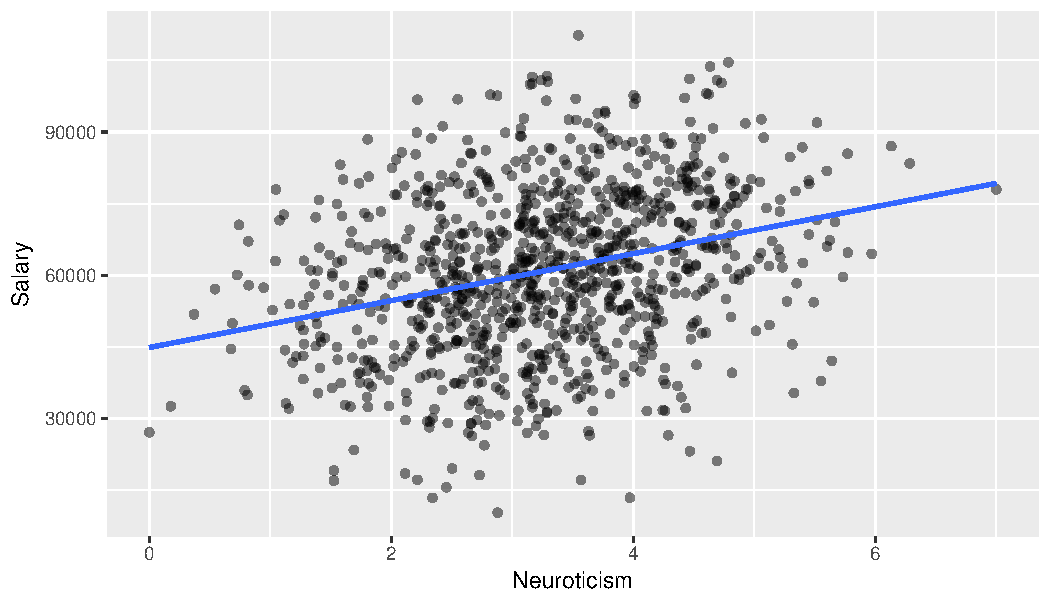
\includegraphics[width=\maxwidth]{figure/multi_4-1} 

}



\end{knitrout}

Now we run a multiple regression analysis. We assume that one very important cause of how much people earn is their educational background. If we include both Education and Neuroticism as independent variables and run the analysis, we obtain the following regression equation:

\begin{equation}
salary = 50249  -3176 \times Neuroticism + 20979 \times Education + e
\end{equation}

Note that we now find a \textit{negative} slope parameter for the effect of Neuroticism! This implies there is a relationship in the data where neurotic employees earn \textit{less} than their less neurotic colleagues! How can we reconcile this seeming paradox: which result should we trust: the one from the simple regression, or the one from the multiple regression?

The answer is: neither. Or perhaps: both! Both analyses give us different information.

Let's look at the last equation more closely. Suppose we make a prediction for a person with a low educational background (Education=0). Then the equation tells us that the expected salary of a person with neuroticism score of 0 is around 50249, and of a person with a neuroticism score of 7 is around 28019. So for employees with low education, the more neurotic employees earn less! If we do the same exercise for average ecudation and high education employees, we find exactly the same pattern: for each unit increase in neuroticism, the yearly salary drops by 3176 Euros.


It is true that in this company, the more neurotic persons generally earn a higher salary. But if we take into account educational background, the relationship flips around. This can be seen from Figure \ref{fig:multi_4}: looking only at the people with a low educational background (Education=0), then the more neurotic people earn less than they less neurotic colleagues with a similar educational background. And the same is true for people with an average education (Education=1) and a high education (Education=3). Only when you put all employees together in one group, you see a positive relationship between Neuroticism and salary.


\begin{knitrout}
\definecolor{shadecolor}{rgb}{0.969, 0.969, 0.969}\color{fgcolor}

{\centering 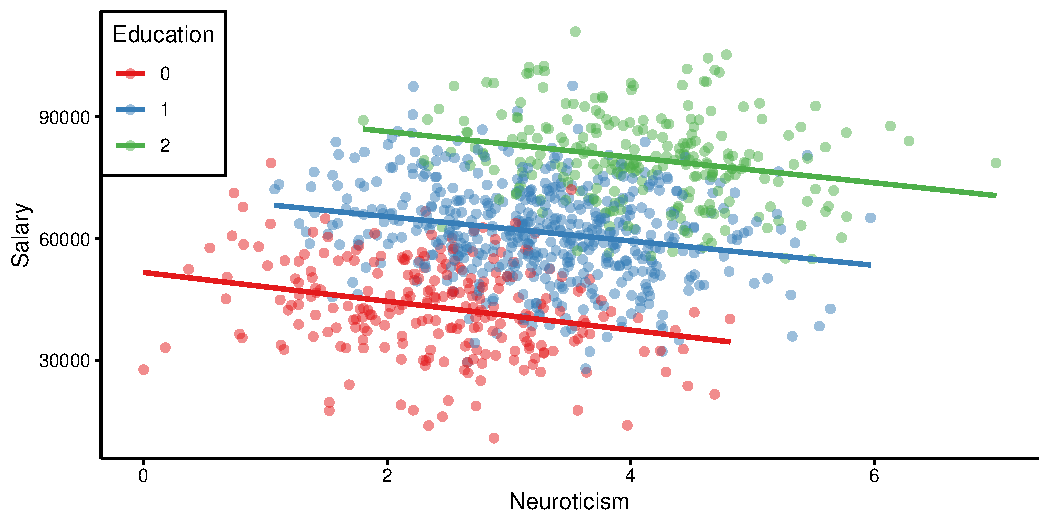
\includegraphics[width=\maxwidth]{figure/multi_5-1} 

}



\end{knitrout}

Simpson's paradox tells us that we should always be careful when interpreting positive and negative correlations between two variables: what might be true at the total group level, might not be true at the level of smaller subgroups. Multiple linear regression helps us investigate correlations more deeply and uncover exciting relationships between multiple variables.


\section{Exercises}


Two neighbours, Elsa and John, are chopping trees in the forest for their respective fireplaces. They pick their trees to chop down, based on the expected volume of wood they can get from that tree. However, Elsa and John disagree on what is the most important aspect of trees for selection. Elsa believes that the tallest tree will give the biggest volume of wood for the fireplace, but John believes that the tree with the largest girth gives the most volume of wood. Luckily there is a data set with three variables: Volume, Girth and Height.


\begin{enumerate}
\item What would the SPSS syntax look like to run a multiple regression, if you want to find out which predictor is most important for the volume of wood that comes from a tree?


\begin{verbatim}
UNIANOVA ....... WITH ........
  /DESIGN = ........
  /PRINT = PARAMETER R-Squared.
\end{verbatim}


\item Suppose you find the output in Table \ref{tab:multi_5}: what would your linear equation look like?

\begin{equation}
\dots \dots = \dots    \dots   \dots \dots \dots \dots+ e
\end{equation}


% latex table generated in R 3.4.2 by xtable 1.8-2 package
% Fri May  4 10:40:29 2018
\begin{table}[ht]
\centering
\caption{Regression table for predicting volume from height and girth.} 
\label{tab:multi_5}
\begin{tabular}{rrrrr}
  \hline
 & Estimate & Std. Error & t value & Pr($>$$|$t$|$) \\ 
  \hline
(Intercept) & -57.9877 & 8.6382 & -6.71 & 0.0000 \\ 
  Girth & 4.7082 & 0.2643 & 17.82 & 0.0000 \\ 
  Height & 0.3393 & 0.1302 & 2.61 & 0.0145 \\ 
   \hline
\end{tabular}
\end{table}





\item On the basis of the output, what would be the predicted volume for a tree with a height of 10 and a girth of 5?

\item On the basis of the output, what would be the predicted volume for a tree with a height of 5 and a girth of 10?

\item For each unit increase of height, how much does the volume increase? Give the approximate 95\% confidence interval for this increase.

\item For each unit increase of girth, how much does the volume increase? Give the approximate 95\% confidence interval for this increase.


\item On the basis of the SPSS output, do you think Lisa is right in saying that height is an important predictor of volume? Explain your answer.

\item On the basis of the SPSS output, do you think John is right in saying that girth is an important predictor of volume? Explain your answer.

\item On the basis of the plots in Figures \ref{fig:multi_7} and \ref{fig:multi_8}, which do you think is the most reliable predictor for Volume: Height or Girth? Explain your answer.

\item How large is the proportion of variance explained in volume, by girth and height?

\item How would you summarize this multiple regression analysis in a research report?

\end{enumerate}

\begin{knitrout}
\definecolor{shadecolor}{rgb}{0.969, 0.969, 0.969}\color{fgcolor}\begin{figure}

{\centering 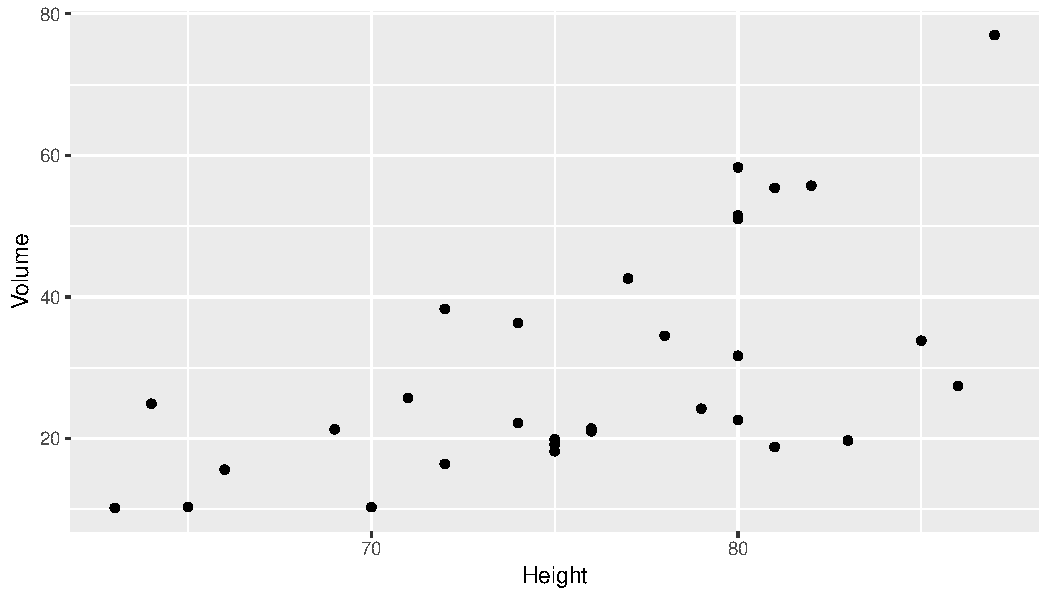
\includegraphics[width=\maxwidth]{figure/multi_7-1} 

}

\caption[A scatterplot for the relationship between height and volume of a tree]{A scatterplot for the relationship between height and volume of a tree.}\label{fig:multi_7}
\end{figure}


\end{knitrout}

\begin{knitrout}
\definecolor{shadecolor}{rgb}{0.969, 0.969, 0.969}\color{fgcolor}\begin{figure}

{\centering 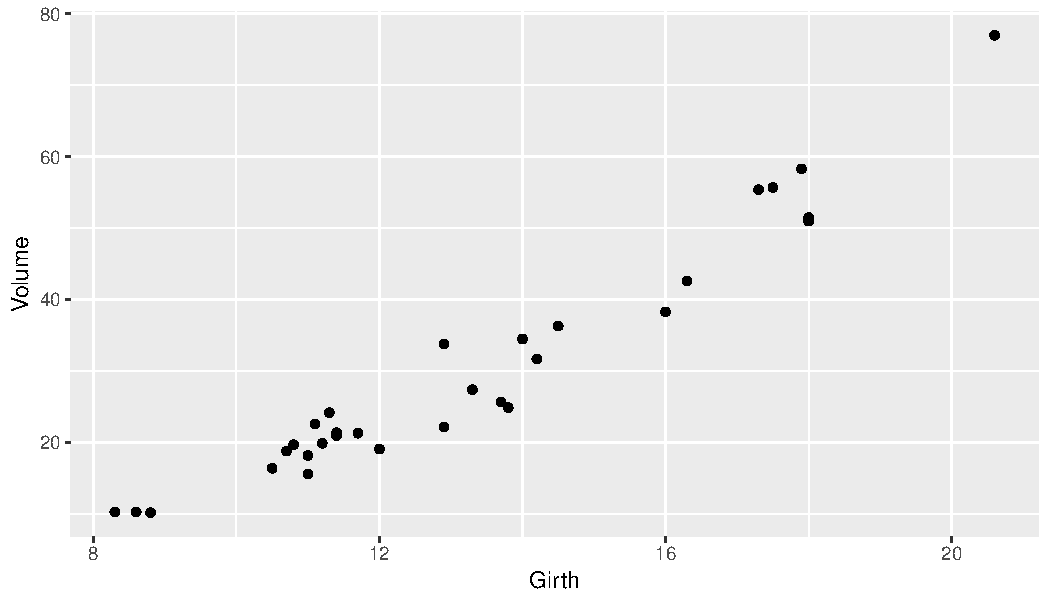
\includegraphics[width=\maxwidth]{figure/multi_8-1} 

}

\caption[A scatterplot for the relationship between girth and volume of a tree]{A scatterplot for the relationship between girth and volume of a tree.}\label{fig:multi_8}
\end{figure}


\end{knitrout}



 % multiple regression


\chapter{Inference I: random samples, standard errors and confidence intervals}

In the previous chapters on simple and multiple regression we have seen how a linear equation can describe a data set: the linear equation describes the behaviour of one variable, the dependent variable, on the basis of one or more other variables, the independent variables. Sometimes we are indeed interested in the relationship between variables in one given data set. For instance, a teacher wants to know whether her exam gradings in her class of last year predict how well they do in a second course a year later.

\begin{knitrout}
\definecolor{shadecolor}{rgb}{0.969, 0.969, 0.969}\color{fgcolor}\begin{figure}

{\centering 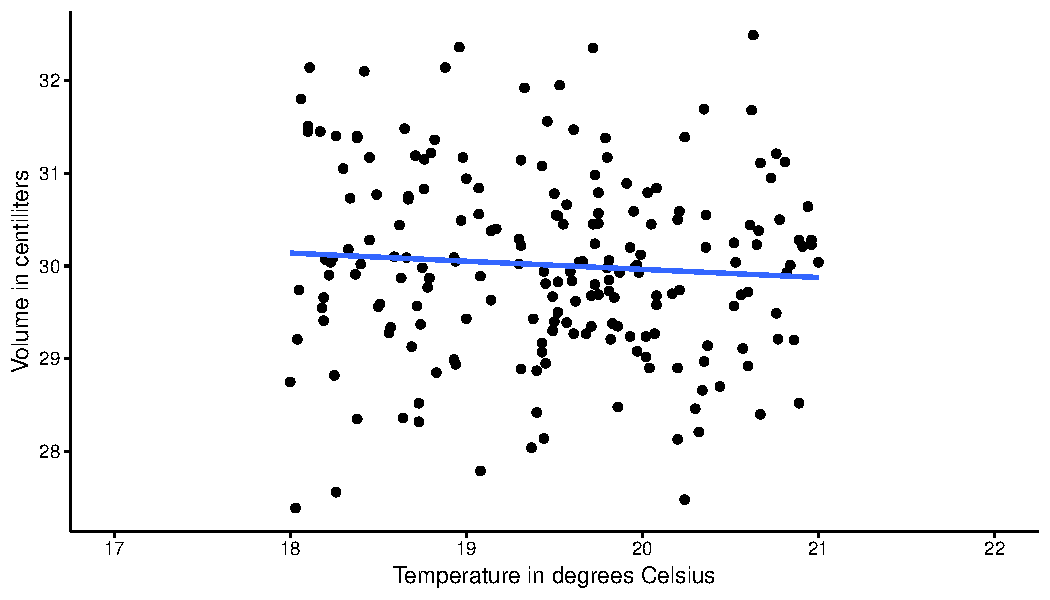
\includegraphics[width=\maxwidth]{figure/inf_0-1} 

}

\caption[The relationship between temperature and volume in a sample of 200 bottles]{The relationship between temperature and volume in a sample of 200 bottles.}\label{fig:inf_0}
\end{figure}


\end{knitrout}


But very often, researchers are not interested in the relationships between variables in one data set, but interested in the relationship between variables in general, not limited to only the observed data. For example, a researcher would like to know what the relationship is between the temperature in a brewery and the volume of beer that goes into one bottle. In order to study the effect of temperature on volume, the researcher measures the volume of beer in 200 bottles and determines from log files the temperature in the factory during production for each measured bottle. The researcher might find a small effect of temperature ($t$) on the volume of beer in the 200 produced bottles. The linear equation might be $volume = 31.7225839 -0.0879535 \times t + e$, see Figure \ref{fig:inf_0}. But the question is what the effect of temperature is in \textit{all} bottles.



In other words, we might have data on a sample of bottles, but we might really be interested to know whether there is an effect \textit{had we been able to measure the volume in all bottles}.


\section{Population data and sample data}

In the beer bottle example above, the volume of beer was measured in a total of 200 bottles. Let's do a thought experiment. Suppose we could have access to volume data about all bottles of beer on all days where the factory was operating, including information about the temperature for each day of production. Suppose that the total number of bottles produced is 80,000 bottles. When we plot the volume of each bottle against the temperature of the factory we get the scatter plot in Figure \ref{fig:inf_1}.


\begin{knitrout}
\definecolor{shadecolor}{rgb}{0.969, 0.969, 0.969}\color{fgcolor}\begin{figure}

{\centering 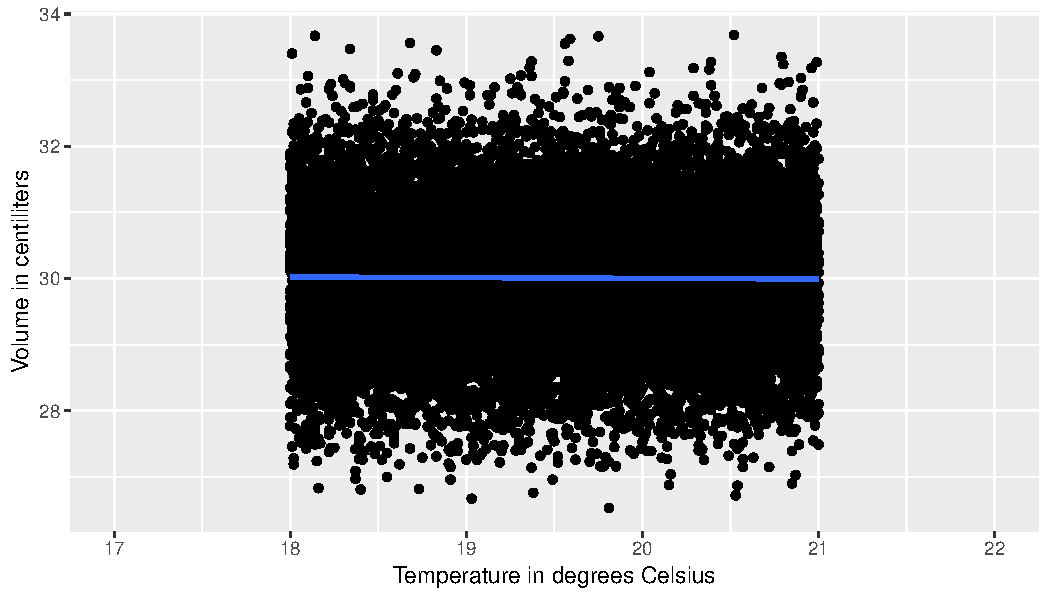
\includegraphics[width=\maxwidth]{figure/inf_1-1} 

}

\caption[The relationship between temperature and volume in all 80,000 bottles]{The relationship between temperature and volume in all 80,000 bottles.}\label{fig:inf_1}
\end{figure}


\end{knitrout}


In our thought experiment, we could determine the regression equation using all bottles that were produced: all 80,000 of them. We then find the blue regression line displayed in Figure \ref{fig:inf_1}. Its equation is $Volume = 29.9769894 + 0.0012583 \times t$.


However, in the data example above, data was only collected on 200 bottles. These bottles were randomly selected: there were many more bottles but we could measure only a limited number of them. This explains why the regression equation based on the sample differed from the regression equation based on all bottles: we only see part of the data.

Here we see a discrepency between the regression equation based on the sample, and the regresssion equation based on the population. Here, the \textit{population} is the collection of all bottles produced in the factory. The \textit{sample} is the collection of 200 randomly selected bottles. Here we have a slope of 0.0012583 in the population, and we see a slope of -0.0879535 in the sample. To distinguish between the two, the population slope is often denoted by the Greek letter $\beta$ and the sample slope by the Roman letter $b$.



\begin{eqnarray}
Population: Volume &=& 29.9769894 + 0.0012583 \times t  \nonumber\\
Sample: Volume &=&  31.7225839  -0.0879535 \times t \nonumber
\end{eqnarray}

The discrependency here is simply the result of chance: had we selected another sample of 200 bottles, we probably would have found a different linear equation with a different slope. The intercept and slope based on sample data, are the result of chance. The population intercept and slope (the true ones) are fixed, but unknown. If we want to know something about the population intercept and slope, we only have the sample equation to go on. Our best guess for the population equation is the sample equation, but how certain can we be about how close the sample intercept and slope are to the population intercept and slope?


\section{Random sampling and the standard error}


In order to know how close the intercept and slope in a sample are to their values in the population, we do another thought experiment. Let's see what happens if we take more than one random sample of 200 bottlees. With random, we mean that every bottle has the same chance of being picked.

We put the 200 bottles that we selected earlier back into the population and we again blindly pick a new collection of 200 bottles. We then measure for each bottle the volume of beer it contains and we determine the temperature of the factory on the day of its production. We then apply a regression analysis and determine the intercept and the slope. Next, we put these bottles back into the population and draw a next random sample of 200 bottles.

You can probably imagine that if we repeat this procedure of randomly picking 200 bottles from a large population of 80,000, each time we find a different intercept and a different slope. Let's carry out this procedure 100 times by a computer. If we then plot the 100 sample intercepts and sample slopes we get the picture in Figure \ref{fig:inf_3}.



\begin{knitrout}
\definecolor{shadecolor}{rgb}{0.969, 0.969, 0.969}\color{fgcolor}\begin{figure}

{\centering 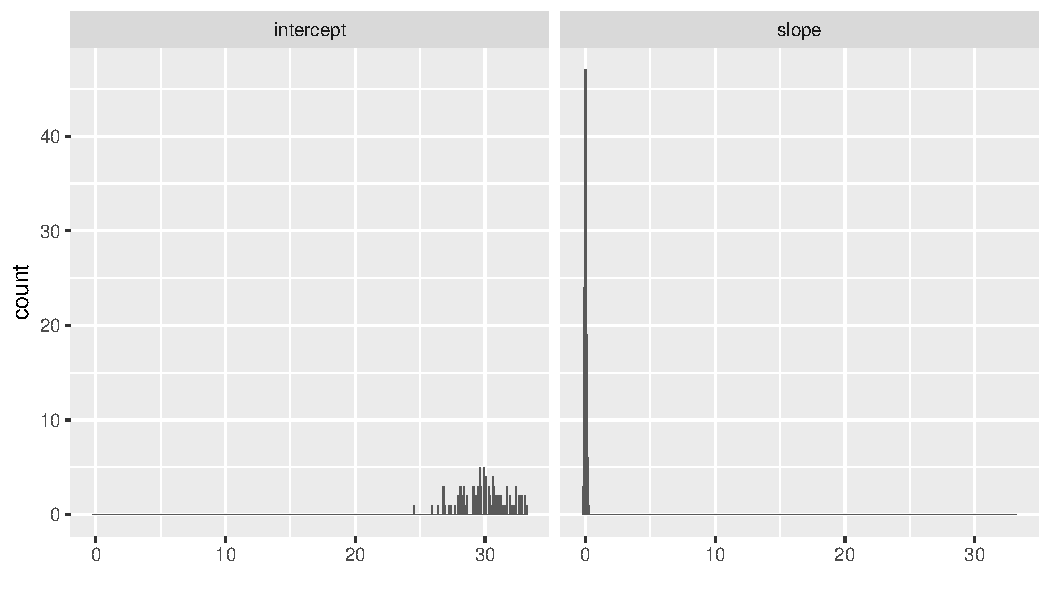
\includegraphics[width=\maxwidth]{figure/inf_3-1} 

}

\caption[Distribution of the sample mean when population variance is 225 and sample size equals 200]{Distribution of the sample mean when population variance is 225 and sample size equals 200.}\label{fig:inf_3}
\end{figure}


\end{knitrout}

We see a large variation in the intercepts that we find, and only a small variation in the slopes (all values very close to 0).


For now, let's focus on the slope; this because we are mostly interested to know whether there is a relationship between volume and temperature, but everything that follows also applies to the intercept. In Figure \ref{fig:inf_5} we see the histogram of the slopes if we carry out the random sampling 1000 times.

\begin{knitrout}
\definecolor{shadecolor}{rgb}{0.969, 0.969, 0.969}\color{fgcolor}\begin{figure}

{\centering 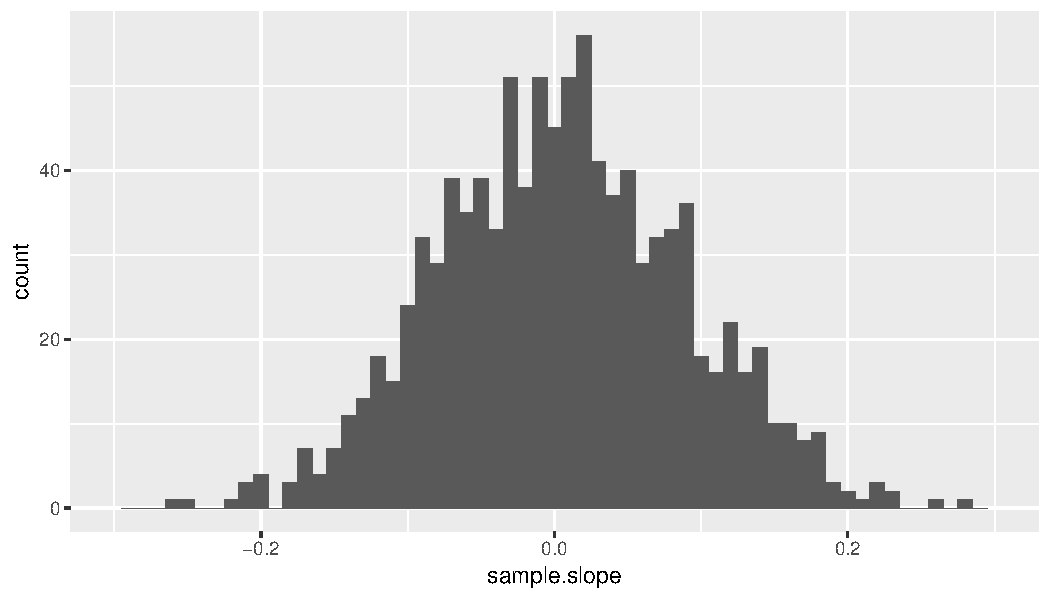
\includegraphics[width=\maxwidth]{figure/inf_5-1} 

}

\caption[Distribution of the sample mean when population variance is 225 and sample size equals 200]{Distribution of the sample mean when population variance is 225 and sample size equals 200.}\label{fig:inf_5}
\end{figure}


\end{knitrout}

If we look at the distribution of the 1000 sample slopes in Figure \ref{fig:inf_5}, we see that on average the sample slope is around $0.0012583$, which is the population slope (the slope if we analyse all bottles). But there is variation around that mean of 0: the standard deviation of all 1000 sample slopes turns out to be 0.0840496.

The standard deviation of the sample mean is called the $0.0012583$. Had the population slope been 110 or -40, the sample slopes would cluster around 110 or -40, but the standard deviation of the sample slopes, the standard error, would be the same.

The standard error for a sample slope represents the uncertainty about the population slope. If the standard error is large, it means that if we would draw many different random samples from the same population data, we would get very different sample slopes. If the standard error is small, it means that if we would draw many different random samples from the same population data, we would get sample slopes that are very close to one another, and very close to the population slope.

It turns out that the standard error for a sample slope depends on many things, but the most important factor is the \textit{sample size}: how many bottles there were in each random sample. In the above example, the sample size is 200 bottles.

% In the above bottle example, the standard deviation of all 80,000 volumes was sd(bottles$volume), where most of the volumes (roughly 95\%) lie between 28 and 32 cl. The variance is the square of the standard deviation so the variance is var(bottles$volume). Now imagine that we have another population, say bottles from a different brand, where we see a much smaller variation in volumes: suppose the average volume is also 30, but the standard deviation is 0.5, so that roughly 95\% of the scores lie between 29 and 31. If we then take 1000 samples from this distribution of bottles from this other brand, we get the distribution in Figure \ref{fig:inf_6}.

% <<inf_6 ,fig.height=4, echo=FALSE, fig.align='center', fig.cap='Distribution of the sample mean when population variance is 25 and sample size equals 200.'>>=
% set.seed(1234)
% bottles <- data.frame(ID=1:800000,
%                       volume= round(rnorm(800000, 30, 0.5 ),2),
%                       temperature=  round(runif(800000, 18,21 ),2)                 )
% sample.intercept <- c()
% sample.slope <- c()
% for (i in 1:1000)
% {
%         sample <- bottles[sample(1:80000,200),]
%         out <- lm(volume~temperature, sample)
%         sample.intercept[i] <- out$coef[1]
%         sample.slope[i] <- out$coef[2]
% }
% data.frame(sample.slope) %>% ggplot(aes(x=sample.slope)) +geom_histogram(binwidth = 0.01) +  xlim(c(-0.3,0.3))
% @

% Now we see that the sample slopes cluster much closer around the value of 0. The standard deviation of this distribution, that is, the standard error, is now much smaller: sd(sample.slope). This makes sense: the larger the variation at population level, the higher the probability that you find extreme values in your sample that influence the sample slope upwards or downwards. The smaller the variation at population level, the higher the proportion of data points in your sample that are very close to the population slope, so that the sample intercept will be very close to the population slope In sum: the higher the population variance, the larger the standard error, the larger the uncertainty about the population slope.

Imagine that you draw only 2 bottles from a population of bottles. Then there is quite some probability that by sheer luck you find one bottle with a low temperature and a small volume, and another bottle with a high temperature and a large volume. This would yield a sample slope that is quite large and positive. But there is also an equally high probability that you get one bottle with a low temperature with a large volume, and another bottle with a high temperature and a small volume. Then based on these two other bottles, the sample slope will be large and negative. In case of a sample size of only 2, you see that there will be quite a lot of variation in the sample slope if we draw various random samples. This large variation in sample slopes is then captured by the standard error, that will be large. With only 2 bottles per sample, the uncertainty about the population slope will then also be large.

Now imagine that your sample size is 20. Then the probability that the 20 bottles will result in a large variation of slopes will be smaller: it would be very unlikely that \textit{all} 20 bottles have either a high volume and a high temperature, or a low volume and a low temperature. If there happen to be a few of such bottles in the sample, the other bottles will average these effects out. Because of this averaging effect, the slope based on 20 bottles will then be closer to the population slope. The standard error therefore decreases with increasing sample size.

In Figure \ref{fig:inf_7} we see the distributions of the sample slope where the sample size is either 2 (left panel) or 20 (right panel). We see quite a lot of variation in sample slopes with sample size equal to 2, and considerably less variation in sample slopes if sample size is 20. This shows that the larger the sample size, the smaller the standard error, the larger the certainty about the population slope.


\begin{knitrout}
\definecolor{shadecolor}{rgb}{0.969, 0.969, 0.969}\color{fgcolor}\begin{figure}

{\centering 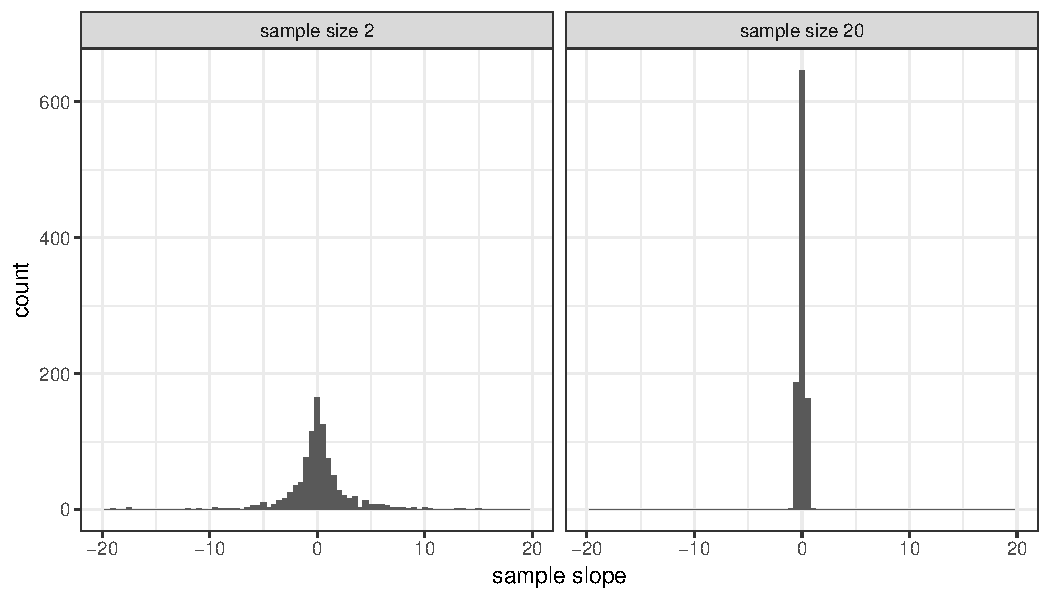
\includegraphics[width=\maxwidth]{figure/inf_7-1} 

}

\caption[Distribution of the sample slope when sample size is 2 and when sample size is 20]{Distribution of the sample slope when sample size is 2 and when sample size is 20.}\label{fig:inf_7}
\end{figure}


\end{knitrout}




So if we have a small standard error, we can be relatively certain that our sample slope is close to the population slope. Above we've done a thought experiment where we knew everything about the population intercept and slope, and we drew 1000 samples from this population. In reality, we don't know anything about the population: we only have the sample data to go on. So suppose we draw a sample of 200 from an unknown population of bottles, and we find a slope of 1, we have to look at the standard error to know how close that sample slope is to the population slope.

For example, suppose we find a sample slope of 1 and the standard error is equal to 0.1. Then we know that the population slope is more likely to be in the neighbourhood of values like 0.9, 1, or 1.1 than in the neighbourhood of 10 or -10.

Now suppose we find a sample slope of 1 and the standard error is equal to 10. Then we know that the sample slope is more likely to be somewhere in the neighbourhood of values like -9, 1 or 11, than around values in the neighbourhood of -100 or +100. However, values like -9, 1 and 11 are quite far apart, so actually we have no idea where the population slope is; we don't even know whether the population slope is positive or negative! The standard error is simply too large.


As we have seen, the standard error depends very much on sample size. Apart from sample size, the standard error for a slope also depends on the variance of the independent variable, the variance of the dependent variable, and the correlations between the independent variable and other independent variables in the equation (in case of multiple regression). We will not bore you with the complicated formula for the standard error for regression coefficients \footnote{See https://www3.nd.edu/~rwilliam/stats1/x91.pdf for the formula. In this pdf, 'IV' means independent variable}. Instead, we look at the standard error that SPSS or other computer packages compute for us.



% % \begin{equation}
% % \sigma_{\bar{y}} = \frac{\sigma}{\sqrt{n}}
% % \end{equation}
% %
% % where $\sigma$ is the population standard deviation and $n$ is sample size. Sample size we know, this is 100, but how about the population standard deviation? We don't know anything about the population, that's the whole reason that we took a sample. But we do know the standard deviation in the sample data. It turns out the \textit{sample standard deviation} $s$ is a rough approximation of the population variance. Therefore we often see the following formula for a standard error
% %
% % \begin{equation}
% % \sigma_{\bar{y}} = \frac{s}{\sqrt{n}}
% % \end{equation}
% %
% %
% % where $s$ represents an approximation of the population standard deviation using the sample data, more specifically the sums of squares (SS, see Chapter 1).
% % \begin{equation}
% % s = \sqrt{\frac{SS}{n-1}}
% % \end{equation}
% %
% % Note the similarity between the standard deviation of a particular set of values, $\sigma=\sqrt{\frac{SS}{n}}$ and the formula for $s$: if you're interested in the standard deviation for a specific set of values, then you use $\sigma=\sqrt{\frac{SS}{n}}$, if you're interested in the standard deviation of the population that a set of numbers is a random sample of, then you use $s=\sqrt{\frac{SS}{n-1}}$.\footnote{Confusingly, $s$ is often called the $sample standard deviation$, while it is really an approximation of the population standard deviation based on the sample data.}
% %
% % Suppose in the Paris data we find an $s$ of 12, then we know that the standard error is equal to $\frac{12}{\sqrt{100}}=12/10$.



\section{$t$-distributions}

Above we saw that if there is a large collection of data points (population) with a particular slope that describes the relationship between two variables, and if you then take random samples out of this collection, each time you find a different value for the slope in the sample, the sample slope. We saw that the standard deviation of the distribution of all such slopes is called the standard error. The standard error gives us information about how certain we can be that a slope in the sample is close to the slope in the population. The smaller the standard error the more certain that the population slope has a value that is in the neighboorhood of the value for the sample slope.



\begin{knitrout}
\definecolor{shadecolor}{rgb}{0.969, 0.969, 0.969}\color{fgcolor}\begin{figure}

{\centering 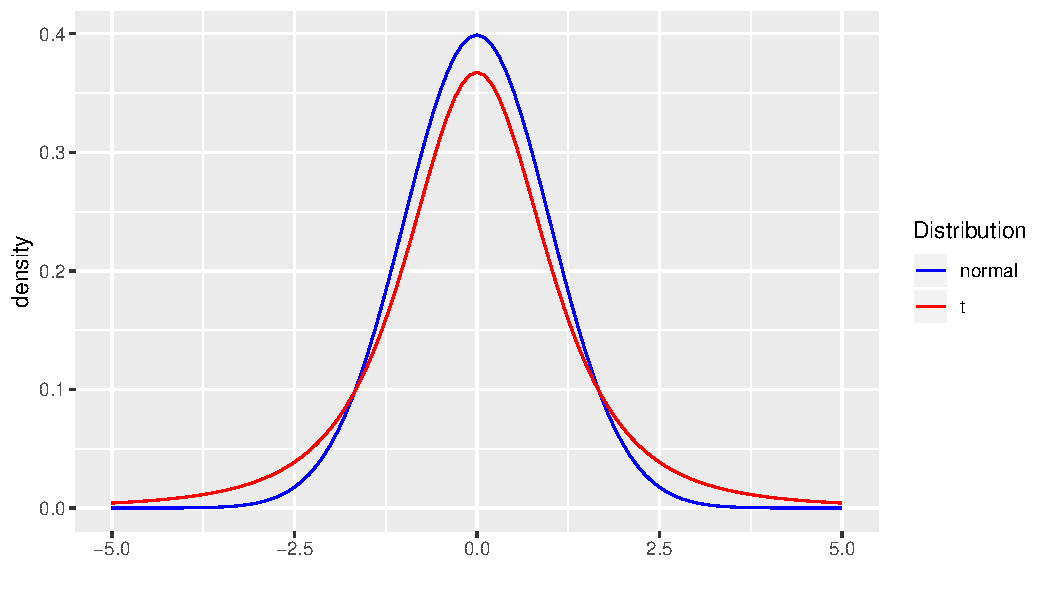
\includegraphics[width=\maxwidth]{figure/inf_8-1} 

}

\caption[Difference in the shapes of a normal distribution and a t-distribution]{Difference in the shapes of a normal distribution and a t-distribution}\label{fig:inf_8}
\end{figure}


\end{knitrout}



When we look at the distribution of the sample slope, for instance in Figure \ref{fig:inf_5}, we notice that the distribution looks very much like a normal distribution. Well, actually it isn't quite a normal distribution. In reality it has the shape of a $t$-distribution. Figure \ref{fig:inf_8} shows the difference between a $t$-distribution (in red) and a normal distribution (in blue). In this figure, the means are equal (0) and the areas under the curve are equal (1), but the shapes are clearly different. Compared to the $t$-distribution, the normal distribution has more observed values close to the mean (the distribution is more peaked). The $t$-distribution has relatively more observations in the tails of the distribution (heavy tails).



Actually, the shape of the distribution of sample slopes depends on the size of the samples. In Figure \ref{fig:inf_9} we see what the distribution would look like if all samples would be of size 4 (the red line) and what the distribution would like like if the samples would be of size 200 (the blue line). Remember: we are talking here only about the \textit{shape} of the distribution. If sample size is large, like for instance 200 (the blue line), the shape looks extremely close to the normal distribution.


In summary, when we draw many samples from a population, the shape of the distribution of sample slopes is that of a $t$-distribution. The shape of the $t$-distribution depends on sample size. The larger the sample size, the more the shape of the $t$-distribution looks like a normal distribution.


\begin{knitrout}
\definecolor{shadecolor}{rgb}{0.969, 0.969, 0.969}\color{fgcolor}\begin{figure}

{\centering 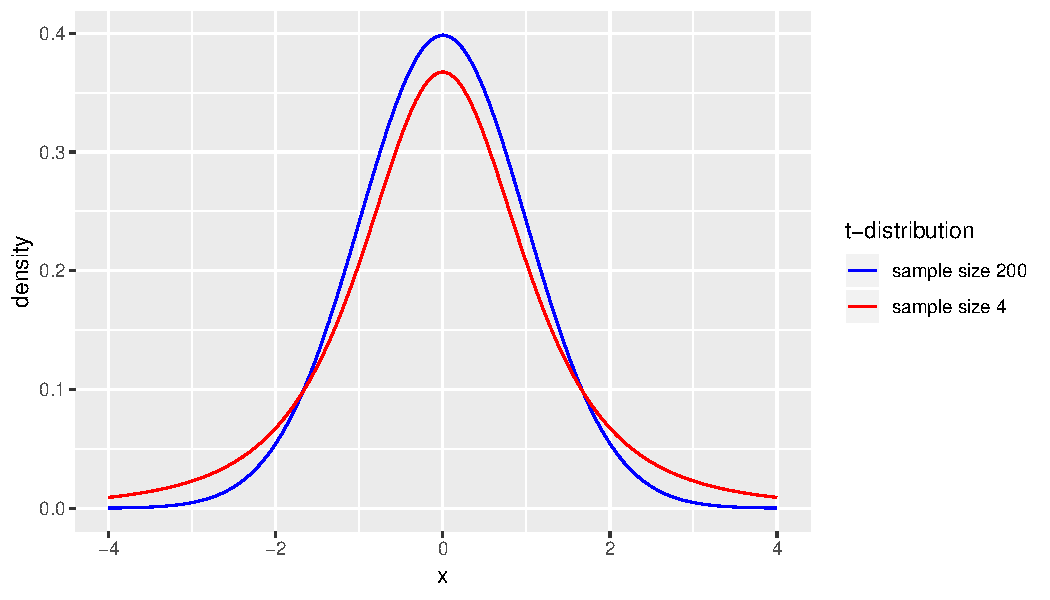
\includegraphics[width=\maxwidth]{figure/inf_9-1} 

}

\caption[The shape of the distribution of sample slopes depends on sample size]{The shape of the distribution of sample slopes depends on sample size.}\label{fig:inf_9}
\end{figure}


\end{knitrout}





\section{$T$-statistics}


Above we saw that sample slopes have a $t$-distribution, and that if sample size is large, say larger than 200, the $t$-distribution looks very much like a normal distribution. From the normal distribution, we know that if we standardize the scores by computing $z$-scores, that is, if we subtract the mean and then divide by the standard deviation, $z= \frac{x-\bar{x}}{\sigma}$, then 2.5\% of the $z$-values is smaller than -1.96 and 2.5\% of the $z$-values is larger than +1.96.


Therefore, if for large sample size the $t$-distribution is practically indistinguishable from the normal distribution, we know that if we standardize the sample slope values, we get a similar result. Instead of looking at the raw slope value, we can compute a standardized slope, let's call that standardized result $t$. Then we get:


\begin{equation}
t = \frac{b-\beta}{se}
\end{equation}

In words: we take a particular sample slope $b$ and we subtract the population slope $\beta$. The result we divide by the standard deviation of the sample slopes, which is callled the standard error $se$.


Let's go back to the example of the beer bottles. In our first random sample of 200 bottles, we found a sample slope of -0.0879535. We also happened to know the population slope, which was 0.0012583. From our computer experiment, we saw that the standard deviation of the sample slopes with sample size 200 was equal to 0.0840496. Thus, if we fill in the formula for the standardized slope $t$, we get for this particular sample


\begin{equation}
T = \frac{-0.0879535-0.0012583}{0.0840496}= -1.0614181
\end{equation}


Notice that we distinguish between a variable $t$ that has a $t$-distribution, and a $T$-statistic that is based on a computation.


Now, what can we say about this $T$-value? Since with a sample size of 200 the distribution closely resembles a normal distribution, we can use normal tables published online or in computer packages to see how likely a value of $T=-1.0614181$ actually is. In normal tables we find that a Z-value of $-1.0614181$ is not that strange: in the standard normal distribution, $14.4249958$\% of the values is smaller than $-1.0614181$. The area is shown in Figure \ref{fig:inf_9b}.


\begin{knitrout}
\definecolor{shadecolor}{rgb}{0.969, 0.969, 0.969}\color{fgcolor}\begin{figure}

{\centering 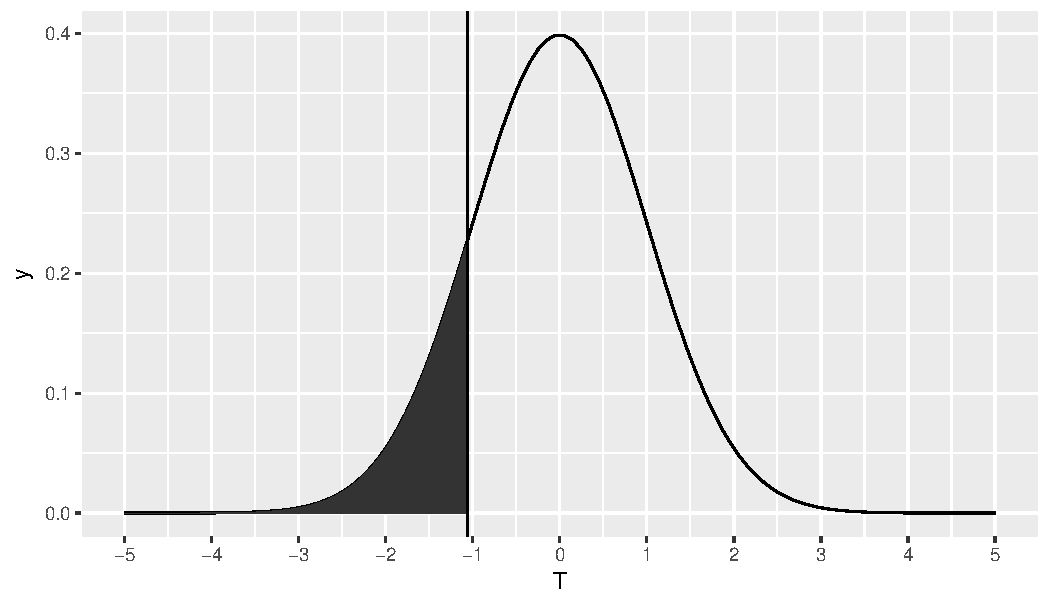
\includegraphics[width=\maxwidth]{figure/inf_9b-1} 

}

\caption[The standard normal distribution and the probability of a Z-score lower than -1.06]{The standard normal distribution and the probability of a Z-score lower than -1.06}\label{fig:inf_9b}
\end{figure}


\end{knitrout}


When would we say that a certain $T$-value would cause concern? Well, perhaps we could say that if the $T$-value we would find were 3 standard deviations away from the population value, either 3 standard deviations above the population value or 3 standard deviations below the population value. From the normal tables, we know that that happens in only $0.2699796$\% of the time.

Alternatively, we could say that we would perhaps also be worried if the sample slope were 2 standard deviations away from the population slope, corresponding to $T$-value of 2 or -2. We know that the probabilty that that happens is around 5\%, small enough perhaps to raise concern about our knowledge about the population slope.

In this section, when discussing $T$-statistics, we assumed we knew the population slope, that is, the slope of the linear equation based on all 80,000 bottles. In reality, we never know the population slope: the whole reason to look at the sample slope is to have an idea about the population slope. Let's look at some hypothetical population slopes.





\section{Hypothetical population slopes}


Since we don't know the actual value of the population slope, we could ask the personnel in the beer factory what they think is a likely value for the slope. Suppose Mark says he believes that a slope of 2 could be true. Well, let's find out whether that is a reasonable guess. Now we \textit{assume} that the population slope $\beta$ is 2, and we compute the $T$-statistic for our sample slope:



\begin{equation}
T = \frac{-0.0879535-2}{0.0840496}= -24.8419251
\end{equation}

From the normal distribution, we know that such a $T$-value is very unlikely: the probability of finding a sample slope 26 standard deviations away form a population slope of 2 is less than 0.00000000000000000000000000001. Because we know that such a $T$-value of 26 is unlikely, we know that a sample slope of -0.0879535 is unlikely \textit{if the population slope is equal to 2}.


Now let's ask Martha. She thinks a reasonable value for the population slope is 0, as she doesn't believe there is a linear relationship between temperature and volume. She feels that the fact that we found a sample slope that was not 0 was a pure coincidence. Based on that hypothesis, we compute $T$ again and find:


\begin{equation}
T = \frac{-0.0879535-0}{0.0840496}= -1.0464475
\end{equation}

In other words, if we believe Martha, our sample slope is only about 1 standard deviation away from her hypothesized value. That's not a very bad idea, since from the normal distribution we know that a value more than 1.05 standard deviations away from the mean (above or below) is $29.54$\%. In other words, if the population is truly 0, then our sample slope of $-0.0879535$ is quite a reasonable finding. If we reverse this line of reasoning: if our sample slope is $-0.0879535$, with a standard error of $0.0840496$, then a population slope of 0 is quite a reasonable guess! It is reasonable, since the difference between the sample slope and the hypothesised value is only $-1.0464475$ standard errors.

So when do we no longer feel that a value for the population slope is reasonable? Perhaps if the probability of finding a sample slope of a certain size given a certain population slope is so small that we no longer believe that the hypothesised value is reasonable. We might for example choose a small probability like 1\%. We know from the normal distribution that 1\% of the values lie at least $-2.5758293$ standard deviations above and below the mean. So if our sample slope is more than $-2.5758293$ standard errors away from the hypothesised population slope, then that population slope is \textit{not} a reasonable guess. In other words, if the \textit{distance} between the sample slope and the hypothesised population slope is more than 2.32 standard errors, then the hypothesised population slope is no longer reasonable.

This implies that any value within the range of $-2.5758293$ standard errors around the sample slope is a collection of reasonable values for the population slope.

Thus, in our example of the 200 bottles, a sample slope of $-0.0879535$ and a standard error of $0.0840496$, the interval from $-0.2829485$ to $0.1070416$ contains reasonable values for the population mean. If we would have to guess the value for the population slope, our guess would be that it would lie somewhere between between $-0.2829485$ and $0.1070416$, \textit{if we feel that 1\% is a small enough probability}.

In data analysis, such an interval that contains reasonable values for the population value, if we only know the sample value, is called a \textit{confidence interval}. Here we've chosen to use $-2.5758293$ standard deviations as our cut-off point, because we felt that 1\% would be a small enough probability to dismiss a population value as a reasonable candidate. Such a confidence interval based on this 1\% cut-off point is called a 99\% confidence interval, because in 99\% of the cases the population value will lie in the confidence interval.

One often also sees 95\% confidence intervals, particularly in social and behavioural sciences. Those are intervals that contain the population value in 95\% of the cases. Because with the normal distribution, 5\% of the observations lie more than 1.96 standard deviations away from the mean, the 95\% confidence interval is constructed by subtracting/addding 1.96 standard errors from/to the sample value. Thus, in the case of our bottle sample, the 95\% confidence interval for the population slope is from $-0.0879535- 1.96* 0.0840496$ to $-0.0879535+ 1.96* 0.0840496$, so our population slope should be somewhere between $-0.2526907$ and $0.0767837$. Luckily, this corresponds to the truth, because we happen to know that the population slope is equal to 0.0012583. In real life we don't know the population slope and of course it might happen that the true population value is not within the 95\% confidence interval, but the probability of such an error is rather low, only 5\%.


\section{Confidence intervals for smaller sample sizes}

In the previous section we used the normal distribution to come up with 95\% and 99\% confidence intervals for the slope coefficient. These were constructed using 1.96 and $-2.5758293$ times the standard error, respectively. However, these numbers 1.96 and $-2.5758293$ can only be used when the sample size is large enough to say that the distribution of the sample slope is very close to a normal distribution. Earlier, we saw that the distribution of the sample slope is actually a $t$-distribution, that doesn't look normal at all for small sample sizes.

So for small sample sizes, we need to know the cut-off points that correspond to 5\% and 1\% probabilities for the $t$-distribution.








% In data analysis, one often uses a \textit{confidence interval} to indicate a range of reasonable values for the population value. Here we found a sample slope of 112. Now imagine that 112 were also the population slope. Then if we would draw many random samples of size 100, we know from the computed standard error of 12/10 that roughly 95\% of the sample means would lie between $112 - 2 \times 12/10 = 109.6$ and $112 + 2 \times 12/10 = 114.4$.

% Now suppose that the true population mean were not 112 but 114.4. In that case, if we draw many samples of size 100, we could reasonably find a value of 112, since 95\% of the sample mean would then lie between $114.4 - 2 \times 12/10 = 112$ and $114.4 + 2 \times 12/10 = 116.8$. So even if the true population mean were 112.4, it's very possible that we could find a sample slope of ?. We cannot neglect the possiblity that the true slope is 114.4. Similarly, we cannot neglect the possibility that the true slope is 109.6, because if the true mean were 109.6, 95\% of the sample means of size 100 would lie between $109.6 - 2 \times 12/10 = 107.2$ and $109.6 + 2 \times 12/10 = 112$. So our range of reasonable values for the population slope would be somewhere between 107.2 and 114.4. This range is referred to as the \textit{95\% confidence interval}. The 95\% confidence interval can be computed by subtracting and adding twice the standard error of the mean to the sample mean.


For large sample sizes we can approximate the $t$-distribution by a normal distribution so that we know that 95\% of the observations lie between -1.96 and +1.96 times the standard deviation. For small sample sizes we have to use a $t$-distribution to construct confidence intervals. For small sample sizes, we need to know the particular shape of the distribution to find out where the middle 95\% of the sample means lie.

Figure \ref{fig:inf_10} shows the case for the situation where the population slope is 0 and the sample size is 4. Suppose the standard error is equal to 1. Then this figure shows that roughly 95\% of the sample slopes lie between $\pm$ 3.18 standard errors below and above the mean. In the same figure we also see that if sample size is 200, 95\% of the sample means lie between $\pm$ 1.97 standard errors below and above the mean. This is almost the same as for the normal distribution, where 95\% of the observations lie between $\pm$ 1.96 standard deviations below and above the mean.

Because for every sample size, the middle region where 95\% of the observations lie is different, there are tables available where these values can be found. However, these tables are built-in in every statistical package, so it is far easier to let SPSS construct the 95\% confidence intervals for us.


% latex table generated in R 3.4.2 by xtable 1.8-2 package
% Fri May  4 10:40:47 2018
\begin{table}[ht]
\centering
\caption{Quantiles for the normal and several t-distributions.} 
\label{tab:nonparmixed_4}
\begin{tabular}{rrrrrrr}
  \hline
probs & norm & t198 & t100 & t50 & t10 & t2 \\ 
  \hline
0.0005 & -3.29 & -3.34 & -3.39 & -3.50 & -4.59 & -31.60 \\ 
  0.0010 & -3.09 & -3.13 & -3.17 & -3.26 & -4.14 & -22.33 \\ 
  0.0050 & -2.58 & -2.60 & -2.63 & -2.68 & -3.17 & -9.92 \\ 
  0.0100 & -2.33 & -2.35 & -2.36 & -2.40 & -2.76 & -6.96 \\ 
  0.0250 & -1.96 & -1.97 & -1.98 & -2.01 & -2.23 & -4.30 \\ 
  0.0500 & -1.64 & -1.65 & -1.66 & -1.68 & -1.81 & -2.92 \\ 
  0.1000 & -1.28 & -1.29 & -1.29 & -1.30 & -1.37 & -1.89 \\ 
  0.9000 & 1.28 & 1.29 & 1.29 & 1.30 & 1.37 & 1.89 \\ 
  0.9500 & 1.64 & 1.65 & 1.66 & 1.68 & 1.81 & 2.92 \\ 
  0.9750 & 1.96 & 1.97 & 1.98 & 2.01 & 2.23 & 4.30 \\ 
  0.9900 & 2.33 & 2.35 & 2.36 & 2.40 & 2.76 & 6.96 \\ 
  0.9950 & 2.58 & 2.60 & 2.63 & 2.68 & 3.17 & 9.92 \\ 
  0.9990 & 3.09 & 3.13 & 3.17 & 3.26 & 4.14 & 22.33 \\ 
  0.9995 & 3.29 & 3.34 & 3.39 & 3.50 & 4.59 & 31.60 \\ 
   \hline
\end{tabular}
\end{table}

But let us look at a few regularities. For several probabilities, the corresponding quantiles are presented in Table \ref{tab:table_inf_1} for the standard normal distribution and several $t$-distributions.

The shape of the $t$-distribution is indicated by its \textit{degrees of freedom}. The shape of the distribution of sample slopes when sample size is 200, is a $t$-distribution with 198 degrees of freedom. The shape of the distribution of sample slopes when sample size is 4, is a $t$-distribution with 2 degrees of freedom. In general, the shape of the distribution of sample slopes for sample size $n$, is a $t$-distribution with $n-2$ degrees of freedom. The higher the degrees of freedom, the more the corresponding $t$-distribution looks like a normal distribution. We will come back to degrees of freedom and the $n-2$ rule in the next section.

Table \ref{tab:table_inf_1} shows for instance the cutoff points for 2.5\% and 97.5\% for the normal distribution and the $t$-distribution with 198 degrees of freedom: 1.96 and 1.97 standard deviations (standard errors) respectively. For the $t$-distribution with 100 degrees of freedom, the cutoff point is 1.98 standard errors. This would be the appropriate $t$-distribution for a sample size of 102. But for smaller sample sizes, the increase in number of standard errors goes up quickly: with 50 degrees of freedom (sample size 52), the cutoff is 2.01, for 10 degrees of freedom it is 2.23 and for 2 degrees of freedom it becomes even 4.30 standard errors. Thus, if we have a sample size of 4, we construct a 95\% confidence interval of 4.30 standard errors below the sample slope and 4.30 standard errors above the sample slope.

If you want to have the 99\% confidence interval, you look at the cutoff points for 0.005 and 0.995 which are -2.58 and +2.58, respectively, for the normal distribution, but -9.92 and +9.92 for a $t$-distribution with 2 degrees of freedom. Suppose we sample 4 bottles and find a sample slope of 5 with a standard error of 4, then the 99\% confidence for the slope is from $5-9.92\times 4$ to $5+9.92\times 4$, so from -34.68 to 44.68, which is of course a huge interval. On the other hand, a sample of only 4 bottles is of course very small.

In short, we can look up the cutoff points for 95\%, 99\% and other intervals from tables online, in books, or in statistical packages. Generally, the smaller the sample size, the lower the degrees of freedom, the larger the number of standard errors you need to construct your confidence intervals.


\begin{knitrout}
\definecolor{shadecolor}{rgb}{0.969, 0.969, 0.969}\color{fgcolor}\begin{figure}

{\centering 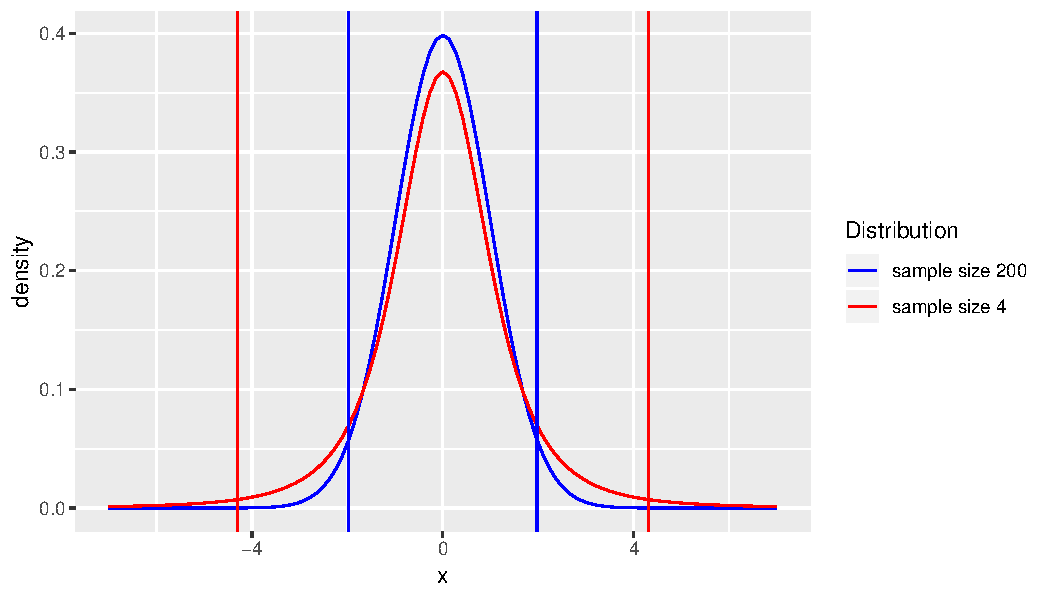
\includegraphics[width=\maxwidth]{figure/inf_10-1} 

}

\caption[Two t-distributions when sample size is 4 or 200, with corresponding 95 percent intervals]{Two t-distributions when sample size is 4 or 200, with corresponding 95 percent intervals.}\label{fig:inf_10}
\end{figure}


\end{knitrout}




\subsection{Exercises}

\begin{enumerate}


\item Suppose we randomly pick 102 students from the University of Twente and determine the linear equation between age (independent variable) and height (dependent variable). Suppose we find a slope coefficient of 0.010, with a standard error of 0.009. Construct the 95\% confidence interval for the slope in the entire population in UT students using table \ref{table_inf_1}.

\item What can we say about values within this constructed confidence interval?

\item Suppose a professor believes the true slope is equal to 0: is that a reasonable belief given the finding of a slope of 0.010? Motivate your answer using the 95\% confidence interval.


\end{enumerate}


Answers:

\begin{enumerate}

\item Sample size is 102, so degrees of freedom for the sample slope is 100. The 95\% cutoff values for the $t$-distribution with 100 degrees of freedom are -1.98 and 1.98. Therefore the 95\% interval ranges from $0.010 - 1.98 \times 0.009$ to $0.010 + 1.98 \times 0.009$, so from -0.008 to 0.028.

\item These values are reasonable values for the population slope.

\item Yes, the value of 0 lies within the range from -0.008 to 0.028, so 0 is a reasonable value for the population slope.




\end{enumerate}
%

\section{Degrees of freedom}


What does the term, "degrees of freedom" mean? It refers to the number of independent pieces of information in a sample of data.

Suppose that we have a sample with four values {4, 2, 6, 8}. There are four separate pieces of information here. There is no particular connection between these values. They are free to take any values, in principle. We could say that there are “four degrees of freedom” associated with this sample of data.

Now, suppose that I tell you that three of the values in the sample are 4, 2, and 6; and I also tell you that the sample average is 5. You can immediately deduce that the fourth value has to be 8. There is no other logical possibility.

So, once I tell you that the sample average is 5, I am effectively introducing a \textit{constraint}. The value of the unknown fourth sample value is implicitly being determined from the other three values, and the constraint. That is, once the constraint is introduced, there are only three logically independent pieces of information in the sample. That is to say, there are only three "degrees of freedom", once the sample average is revealed.

Now let's carry this example to regression analysis. Suppose I have four observations of variables $x$ and $y$. Each value of $y$ is one piece of information. These values could be anything, so we say that we have 4 degrees of freedom. Now suppose I use a linear equation for these data points, and suppose I only use an intercept. Let the intercept be 5. Now the first bit of information, $x$ and $y$ could be anything, say 1 and 2 respectively. The second and third bits of information could also be anything, say 2 and 6, and 4 and 2. Figure \ref{fig:inf_11} shows these bits of information as dots in a scatterplot. Since we know that the intercept is equal to 5, with no slope (slope=0), we can also draw the regression line.

\begin{knitrout}
\definecolor{shadecolor}{rgb}{0.969, 0.969, 0.969}\color{fgcolor}\begin{figure}

{\centering 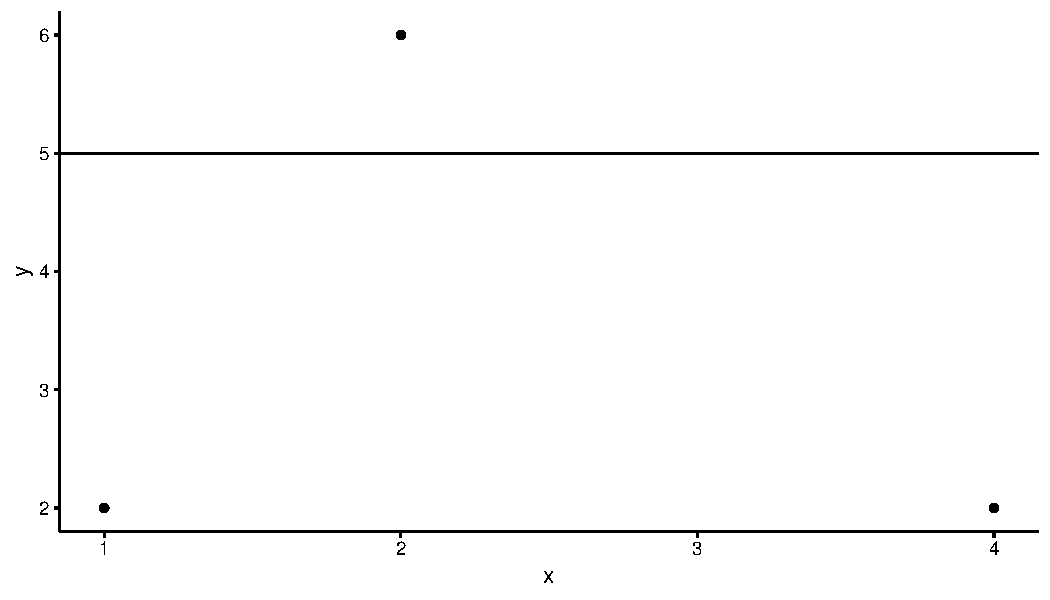
\includegraphics[width=\maxwidth]{figure/inf_11-1} 

}

\caption[Distribution of the sample mean when sample size is 4 or 200]{Distribution of the sample mean when sample size is 4 or 200}\label{fig:inf_11}
\end{figure}


\end{knitrout}

If we compute the residuals, we have residuals -3, 1 and -3 for these data points. When we sum them we get -3. Since we know that all residuals should sum to 0 in a regression analysis, we can derive the fourth residual to be +5, since only then the residuals sum to 0. Therefore, the $y$-value for the fourth data point (for $x=3$, for example) has to be 8, since then the residual is equal to $8-5=3$.

In short, when we do a regression analysis with only an intercept, the degrees of freedom is equal to the number of data points (combinations of $x$ and $y$) minus 1, or in short notation: $n-1$.

Now let's look at the situation where we do a regression analysis with both an intercept and a slope: suppose the intercept is equal to 3 and the slope is equal to 1: $y=3+1 x$. Then suppose we have the same $x$-values as the example above: 1, 2 and 4. When we give these $x$-values corresponding $y$-values, 2, 6, and 3, we get the plot in Figure \ref{fig:inf_12}.

\begin{knitrout}
\definecolor{shadecolor}{rgb}{0.969, 0.969, 0.969}\color{fgcolor}\begin{figure}

{\centering 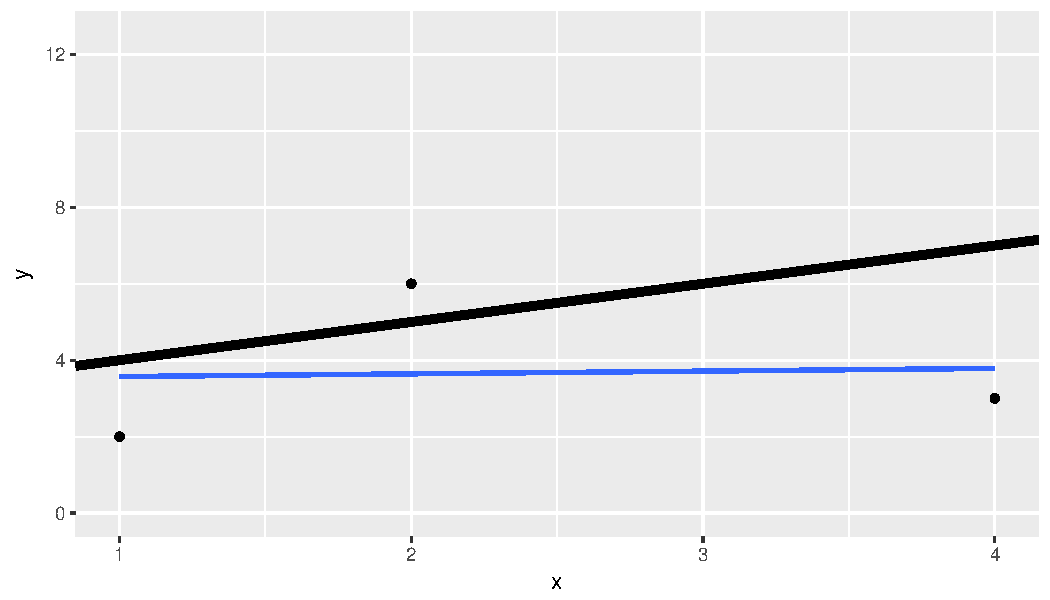
\includegraphics[width=\maxwidth]{figure/inf_12-1} 

}

\caption[Distribution of the sample mean when sample size is 4 or 200]{Distribution of the sample mean when sample size is 4 or 200}\label{fig:inf_12}
\end{figure}


\end{knitrout}

The black line is the regression line that should be imposed on the data. The blue line is the regression line based on the three data points. Now the question is, is it possible for a fourth data point with $x=3$, to think of a $y$-value such that the regression line based on these four data points is equal to $y=3+1x$?

Figure \ref{fig:inf_13} shows a number of possibilities for the value of $y$ if $x=3$. It can be seen, that it is impossible to pick a value for $y$ such that we get a regression equation $y=3+1x$.

\begin{knitrout}
\definecolor{shadecolor}{rgb}{0.969, 0.969, 0.969}\color{fgcolor}\begin{figure}

{\centering 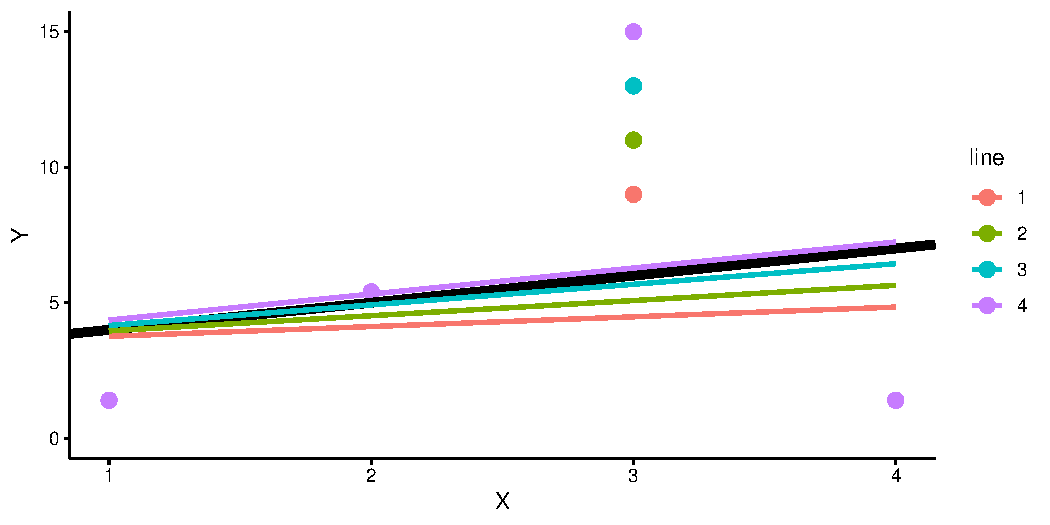
\includegraphics[width=\maxwidth]{figure/inf_13-1} 

}

\caption[Different regression lines for different values of y if x=3]{Different regression lines for different values of y if x=3.}\label{fig:inf_13}
\end{figure}


\end{knitrout}

So, with 4 data points, we can never freely choose 3 residuals in order to satisfy the constraint that a particular regression equation holds. It turns out, that in this case we can only choose 2 residuals freely, and the remaining residuals are already determined. To prove this requires matrix algebra, but the gist of it is that if you have a regression equation with both an intercept and a slope, the degrees of freedom is equal to the number of data points minus 2: $n-2$.

In the more general case of multiple regression, with the number of independent variables equal to $k$ and including an intercept, the degrees of freedom for the $t$-distribution is equal to $n-k-1$. One could also say, the degrees of freedom is equal to sample size minus the number of parameters in your model.

For example, suppose you have 200 data points and 4 independent variables. Then you have 4 slope parameters and 1 intercept parameter in your model, so 5 parameters in total. The degrees of freedom is in that case $n-5=195$.


\chapter{Inference II: hypothesis testing, $p$-values and beyond}

\section{The null-hypothesis}

Often data analysis is about finding an answer to the question whether there is a relationship between two variables. In most cases, the question pertains to the population: is there a relationship between variable y and variable x in the population? In many cases, one looks for a linear relationship between two variables.

One common method to answer this question is to analyse a sample of data, apply a linear model, and look at the slope. However, one then knows the slope in the sample, but not the slope in the population. We have seen that the slope in the sample can be very different from the slope in the population. Suppose we find a slope of 1: does that mean there is a slope in the population or that there is no slope in the population?

In inferential data analysis, one often works with two hypotheses: the null-hypothesis says that the population slope is equal to 0 and the alternative hypothesis says that there is a  slope that is different from 0. Remember that if the slope is equal to 0, that is saying that there is no linear relationship between $x$ and $y$. Therefore, the null-hypothesis states there is no linear relationship between $x$ and $y$ in the population. If there is a slope, whether positive or negative, is the same as saying there is a linear arelationship, so the alternative hypothesis states there that is a linear relationship between $x$ and $y$ in the population. The null-hypothesis is often denoted as $H_0$ and the alternative hypothesis is often denoted as $H_1$. In formula form, we have


\begin{eqnarray}
H_0: \beta_{slope}=0 \\
H_1: \beta_{slope} \neq 0
\end{eqnarray}

So the population slope, $\beta_{slope}$, is either 0 or it is not. Our data analysis is then aimed at determining which of these two hypotheses is true. Key is that we do a thought experiment on the null-hypothesis: we wonder what would happen if the the population slope would be really 0. In our imagination we draw many samples of a certain size, say 40 data points, and then determine the slope for each sample. Earlier we learned that the many sample slopes would form a histogram in the shape of a $t$-distribution with $n-2=38$ degrees of freedom. For example suppose we would draw 1000 samples of size 40, then the histogram of the 1000 slopes would be like depicted in Figure \ref{fig:inf_14}

\begin{knitrout}
\definecolor{shadecolor}{rgb}{0.969, 0.969, 0.969}\color{fgcolor}\begin{figure}

{\centering 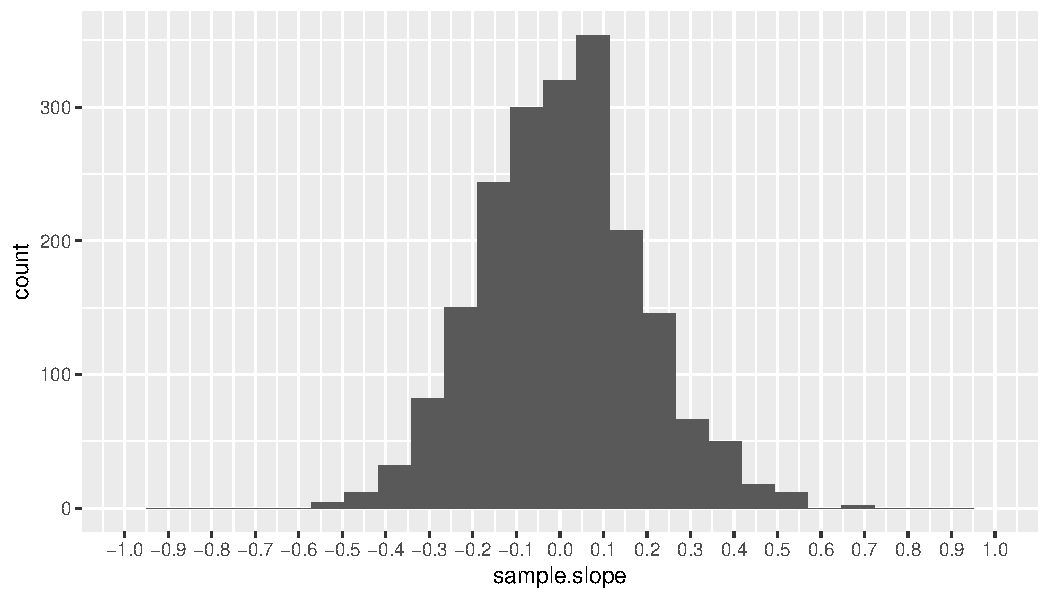
\includegraphics[width=\maxwidth]{figure/inf_14-1} 

}

\caption[Distribution of the sample mean when population variance is 25 and sample size equals 200]{Distribution of the sample mean when population variance is 25 and sample size equals 200.}\label{fig:inf_14}
\end{figure}


\end{knitrout}

From this histogram we see that all observed sample slopes are well between -0.8 and 0.8. This gives us the information we need. Of course, we have only one sample of data, and we don't know anything about the population data. But we do know that if the population slope is equal to 0, then it is very unlikely to find a sample slope of say 1 or 2, or -2 for that matter. Thus, if we happen to find a sample slope of say -2, we know that this finding is extremely unlikely \textit{if we hold the null-hypothesis to be true}. In other words, if the population slope is equal to 0, it would be quite improbable to find a sample slope of -2. Therefore, we regard the null-hypothesis to be false, since it does not provide a good explanation of why we found a slope of -2. In that case, we say that \textit{we reject the null-hypothesis}.

% \section{$T$-statistics}
%
% In previous sections we looked at the distribution of the slope based on sample data, if you draw many random samples from a population of data points. We saw that nearly always, the slope based on your sample data is different from the slope in the population data. We learned that the shape of the distribution is that of a $t$-distribution. The particular shape of the distribution depends on the degrees of freedom, and we learned that the degrees of freedom is equal to the number of data points in your sample (sample size $n$) minus the number of parameters/coefficients in your linear equation.
%
% We said that the distribution of the regression slope has the \textit{shape} of a $t$-distribution. In order to get a $t$-distribution, you have to standardize the scores. Similar to standardizing other scores to z-scores, by subtracting the mean and dividing by the standard deviation, we too standardize slope estimates into T-scores.
%
% Similar to the normal distribution. If you know a value is 2, then you know nothing, but if you know that a value is 20 standard deviations away from the mean, that is, a $z$-score of 20, then you know that such a value is rather unlikely.
%
% The same is true for the distribution of sample slopes. Only knowing that the sample slope is 1, says nothing, but that the slope is 30 standard errors away from a particular value is saying that such a value is unlikely.
%
% So similar to $z$-scores, we subtract the mean from the sample slope and divide by the standard deviation. If the null-hypothesis is true, the mean of the sample slopes is 0. We also know that the standard deviation of the sample slopes is the standard error.
%
% This standardized slope is called a $T$-statistic. A statistic is a quantity that is based on a calculation using your sample data. For example, using least squares, you determine the slope parameter $b_{slope}$, and you determine the standard error $se$. Next, you compute the $T$-statistic:
%
% \begin{equation}
% T = \frac{b_{slope}-0}{se} = \frac{b_{slope}}{se}
% \end{equation}
%
%
% Figure \ref{fig:inf_15} shows the $t$-distribution with $40-2=38$ degrees of freedom. This is the distribution for the $T$-statistic if our sample size is equal to 40 and the true population slope is equal to 0.
%
%
% <<inf_15,fig.height=4, echo=FALSE, fig.align='center', fig.cap='Different regression lines for different values of y if x=3.'>>=
% data.frame(x)  %>%  ggplot(aes(x=x)) +
%   stat_function(fun = dt, args = list(df=38))  +
%         ylab("density") + xlim(c(-4,4)) + xlab("T")
% @
%
% Suppose the true value of the slope (the slope in the population data) is equal to exactly 0. Then if you analyse a sample of 40 data points, you might find a slope of $b_{slope}=1$, and the standard error turns out to be 2. If we then compute $T$, we get $T=\frac{b_{slope}}{se}=1/2=0.5$. In other words, our slope is half a standard error away from the hypothesised value of 0. Whether this is a lot, depends on the shape of the distribution. For this $T$ we know that it has a $t$-distribution with 38 degrees of freedom. Figure \ref{fig:inf_16} shows this distribution. The tails that each contain 2.5\% are shaded. Thus, if the true slope is 0, and if we would draw a lot of samples and for each sample determine the slope, then 95\% of those slopes will lie within the non-shaded area. The figure also indicates the value for our T-statistic, 0.5. It can be clearly seen that a value of 0.5 lies well within the middle 95\% of the distribution, in other words, a value of 0.5 is not that strange for a $t$-distribution with 38 degrees of freedom.
%
%
% <<inf_16,fig.height=4, echo=FALSE, fig.align='center', fig.cap='Different regression lines for different values of y if x=3.'>>=
%
% df = 38; ncp = 0; limits = c(-5,5)
% lb=-20; ub=qt(0.025, df=df, ncp=ncp)
%     x <- seq(limits[1], limits[2], length.out = 100)
%     xmin <- max(lb, limits[1])
%     xmax <- min(ub, limits[2])
%     areax <- seq(xmin, xmax, length.out = 100)
%     area <- data.frame(x = areax, ymin = 0, ymax = dt(areax, df=df, ncp=ncp))
%     (ggplot()
%      + geom_line(data.frame(x = x, y = dt(x, df=df, ncp=ncp)),
%                  mapping = aes(x = x, y = y))
%      + geom_area(data = area, mapping = aes(x = x,  y = ymax))
%      + scale_x_continuous(limits = limits, breaks=seq(-5,5,1))
%      + geom_area(data = area, mapping = aes(x = seq(qt(0.975, df=df, ncp=ncp), 5, length.out = 100),  y = dt(seq(qt(0.975, df=df, ncp=ncp), 5, length.out = 100), df=df, ncp=ncp)))
%             + geom_vline(xintercept = 0.5)  + xlab("T") )
% @
%
%
%
%
%
%
%
%
%
% Based on our reasoning in the section on confidence intervals, we can construct an interval of reasonable values for the population $T$ by taking the middle 95\% of the distribution.

\section{The $p$-value}

The $p$-value is a probability. It represents the probability of observing certain events, given that the null-hypothesis is true.

Earlier we obtained a sample slope of 1, and we saw that this value was 0.5 standard errors away from 0. Thus, the $T$-statistic was 0.5. We looked at the $t$-distribution with 38 degrees of freedom, and saw that such a value of 0.5 was not very strange: it lies well within the middle 95\% of the $t$-distribution.
What is often done is to compute the probability that we obtain such a value of 0.5 or larger. Figure \ref{fig:inf_17} shows the area under the curve for values of $T$ that are larger than 0.5.

\begin{knitrout}
\definecolor{shadecolor}{rgb}{0.969, 0.969, 0.969}\color{fgcolor}\begin{figure}

{\centering 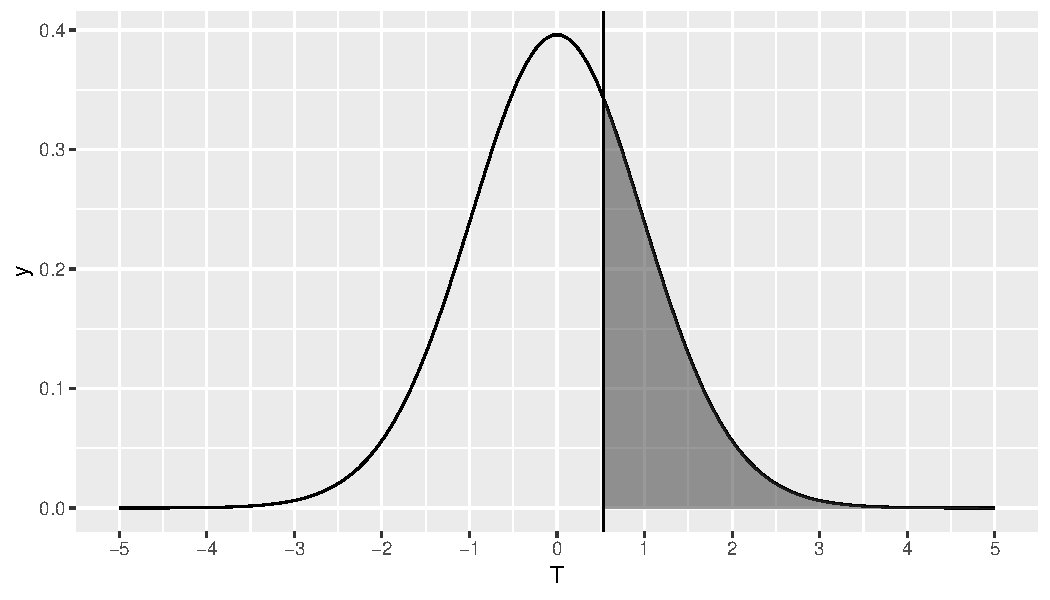
\includegraphics[width=\maxwidth]{figure/inf_17-1} 

}

\caption[Different regression lines for different values of y if x=3]{Different regression lines for different values of y if x=3.}\label{fig:inf_17}
\end{figure}


\end{knitrout}

In tables online, in books, or available in statistical packages, we can look up how large this area is. It turns out to be 0.3099792. So, if the population slope is equal to 0 and we draw an infinite number of samples of size 40 and compute the sample slopes, then 31\% of them will be larger than 0.5. The proportion of the shaded area is what we call a one-sided $p$-value. We call it one-sided, because we only look at one side of the $t$-distribution: we only look at values that are larger than our value of 0.5.

Earlier we observed that a value of 0.5 is not that strange to find if the population slope is 0. On the same token, it would also have been probable to find a slope of -1, corresponding to a $T$-value of -0.5. Since the $t$-distribution is symmetrical, the probability of finding a $T$-value of less than -0.5 is depicted in Figure \ref{fig:inf_18}, and of course this probability is also 0.3099792.

\begin{knitrout}
\definecolor{shadecolor}{rgb}{0.969, 0.969, 0.969}\color{fgcolor}\begin{figure}

{\centering 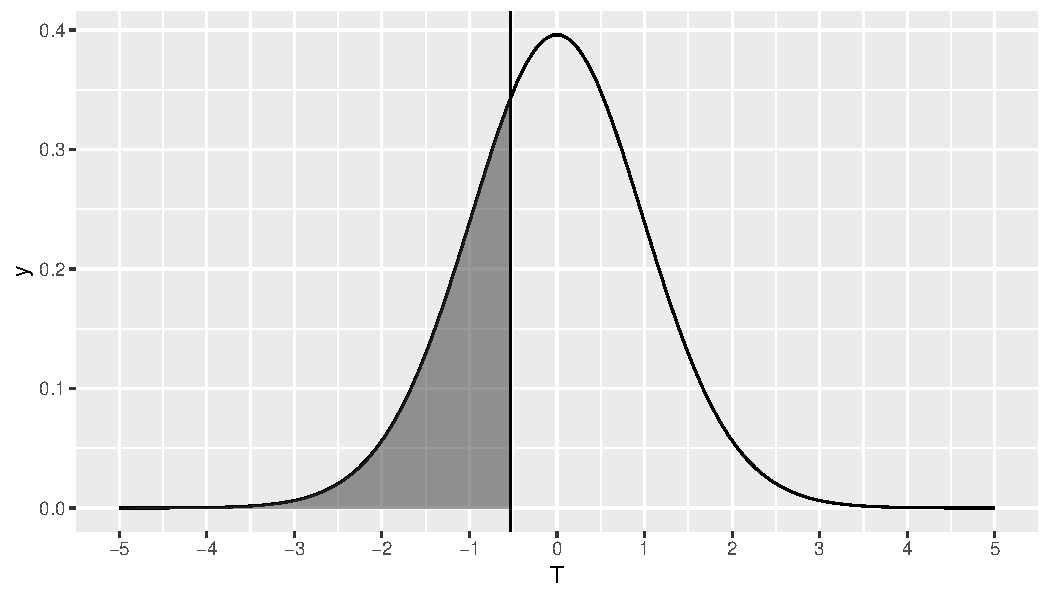
\includegraphics[width=\maxwidth]{figure/inf_18-1} 

}

\caption[Different regression lines for different values of y if x=3]{Different regression lines for different values of y if x=3.}\label{fig:inf_18}
\end{figure}


\end{knitrout}

Remember that the null-hypothesis is that the population slope is 0, and the alternative hypothesis is that the population slope is \textit{not} 0. We should therefore conclude that if we find a very large positive \textit{or} negative slope, large in the sense of the number of standard errors away from 0, that the null-hypothesis is unlikely to be true. Therefore, if we find a slope of 0.5 or -0.5, then we should determine the probability of finding a $T$-value that is larger than 0.5 or smaller than 0.5. This probability is depicted in Figure \ref{fig:inf_19} and is equal to twice the one-side $p$-value, $2 \times 0.3099792=0.6199583$.

\begin{knitrout}
\definecolor{shadecolor}{rgb}{0.969, 0.969, 0.969}\color{fgcolor}\begin{figure}

{\centering 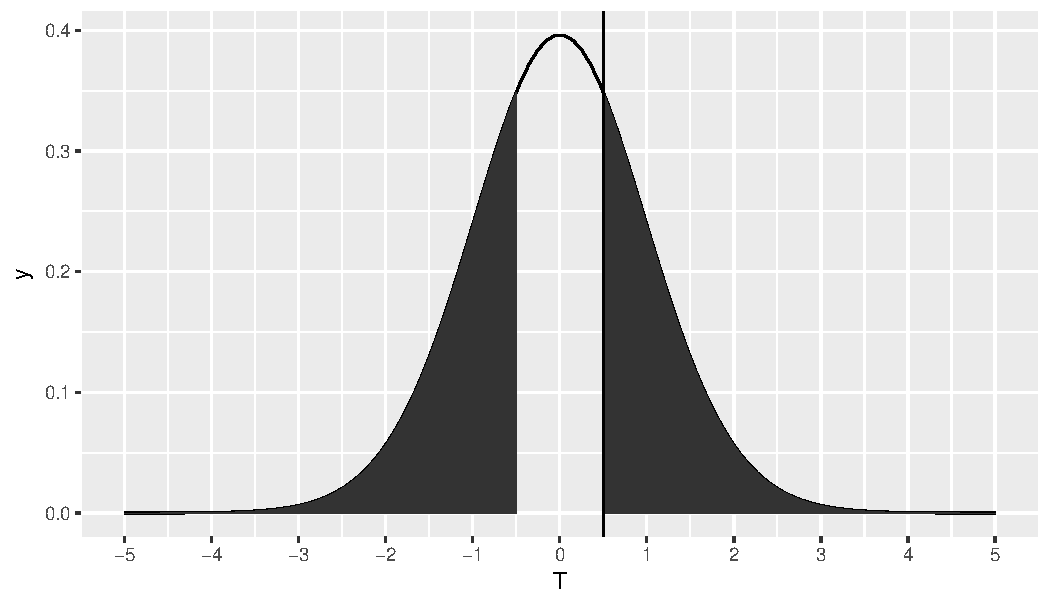
\includegraphics[width=\maxwidth]{figure/inf_19-1} 

}

\caption[Different regression lines for different values of y if x=3]{Different regression lines for different values of y if x=3.}\label{fig:inf_19}
\end{figure}


\end{knitrout}

This probability is called the \textit{two-sided} $p$-value. This is the one that should always be used, since the alternative hypothesis is also two-sided: the population slope can be positive or negative. The question now is: is a sample slope of 1 enough evidence to reject the null-hypothesis? To determine that, we determine how many standard errors away from 0 the sample slope is and we look up in tables how often that happens. Thus in our case, we found a slope that is 0.5 standard errors away from 0 and the tables told us that the probability of finding a slope that is at least 0.5 standard deviations away from 0 (positive or negative) is equal to 0.6199583. We find this probability rather large, so we decide that we \textit{do not reject the null-hypothesis}.


\section{Hypothesis testing}

When do we think the probability is small enough to conclude that the null-hypothesis can be rejected? This was a question posed to the founding father of statistical hypothesis testing, Sir Ronald Fischer. In his book \textit{Statistical Methods for Research Workers} (1925), Fisher proposed a probability of 5\%. He advocated 5\% as a standard level for concluding that there is evidence against the null-hypothesis. However, he did not see it as an absolute rule: "If P is between .1 and .9 there is certainly no reason to suspect the hypothesis tested. If it is below .02 it is strongly indicated that the hypothesis fails to account for the whole of the facts. We shall not often be astray if we draw a conventional line at .05...". So Fisher saw the $p$-value as an informal index to be used as a measure of discrepancy between the data and the null-hypothesis: “The null hypothesis is never proved or established, but is possibly disproved”.


Later, Neyman and Pearson saw the $p$-value as an instrument in decision making: is the null-hypothesis true, or is the alternative hypothesis true? You either reject the null-hypothesis or you don't, there is nothing in between. This view to data-analysis is still rather popular in the social and behavioural sciences, but also in particle physics. In order to make such a black-and-white decision, you decide before-hand, that is, before collecting data, what \textit{level of significance} you choose for your $p$-value to decide whether to reject the null-hypothesis. For example, as your significance level, you might want to choose 1\%. Let's call this chosen significance level $\alpha$. Then you collect your data, you apply your linear model to the data, and find that the $p$-value associated with the slope effect equals $p$. If $p$ is smaller than or equal to $\alpha$ you \textit{reject the null-hypothesis}, and if $p$ is larger than $\alpha$ then you \textit{do not reject the null-hypothesis}. A coefficient with a $p \leq \alpha$ is said to be a \textit{significant} effect, and a coefficient with a $p > \alpha$ is said to be \textit{non-significant}. If the slope is significant, then one should reject the null-hypothesis and say there is a slope in the population different from zero. If the slope is not significant, then one should not reject the null-hypothesis and say there is no slope in the population (i.e., the slope is 0).


Since data-analysis is about probabilities, there is always a chance that you draw the wrong conclusion: you can wrongfully reject the null-hypothesis, or you can wrongfully accept the null-hypothesis. Pearson and Neyman distinguished between two kinds of error: one could reject the null-hypothesis while it is actually true (error of the first kind, or type I error) and one could accept the null-hypothesis while it is not true (error of the second kind, or type II error). The probability of a type I error is the same as our $\alpha$ for the significance level, and the probability of a type II error by $\beta$.


As an example, suppose you want to determine the slope for the effect of age on height in children. The null-hypothesis is that the effect is 0 in the population of all children. You might study a sample of children and you might find a value for the slope. You might decide that if the $p$-value is lower than a critical value you conclude that the null-hypothesis is not true. Suppose you think a probability of 1\% is enough to reject the null-hypothesis as true. In other words, if $p \leq 0.01$ then we no longer think 0 is a reasonable value for the population slope. In this case, we have determined our $\alpha$ or type I error rate to be $\alpha=0.01$. This means that if we study a random sample of children, we look at the slope and find a $p$-value of 0.011, then we do not reject the null-hypothesis, but if we find a $p$-value of 0.010, we reject the null-hypothesis.

Setting the $\beta$ value is bit trickier. It is not possible to to compute the probability that we find a non-significant effect $(p < alpha)$, given that the alternative hypothesis is true, because the alternative hypothesis is only saying that the slope is not equal to 0. In order to compute $\beta$, we need to think first of a reasonable size of the slope that we expect. For example, suppose we believe that a slope of 1 is quite reasonable, given what we know about growth in children. Let that be our alternative hypothesis. Next, we determine the distribution of sample slopes under the assumption that the population slope is 1.
We know that this distribution has a mean of 1 and a standard deviation equal to the standard error.
We also know it has the shape of a $t$-distribution. Let sample size be equal to 102 and the standard error 1. If we standardize the slopes by dividing by the standard error, we get the two $t$-distributions in Figure \ref{fig:inf_20}: one distribution of $T$-values if the population slope is 0, and one distribution of $T$-values if the population slope is 1.
The black areas represent the area where $p < \alpha$: for all values of $T$ smaller than $-2.4285676$ and larger than $2.4285676$, we reject the null-hypothesis. The probability that this happens, \textit{if the null-hypothesis is true}, is equal to $\alpha$ which is 0.01 in this example. The probability that this happens \textit{if the alternative hypothesis is true} (here, population slope is 1), is depicted in Figure \ref{fig:inf_21}.


\begin{knitrout}
\definecolor{shadecolor}{rgb}{0.969, 0.969, 0.969}\color{fgcolor}\begin{figure}

{\centering 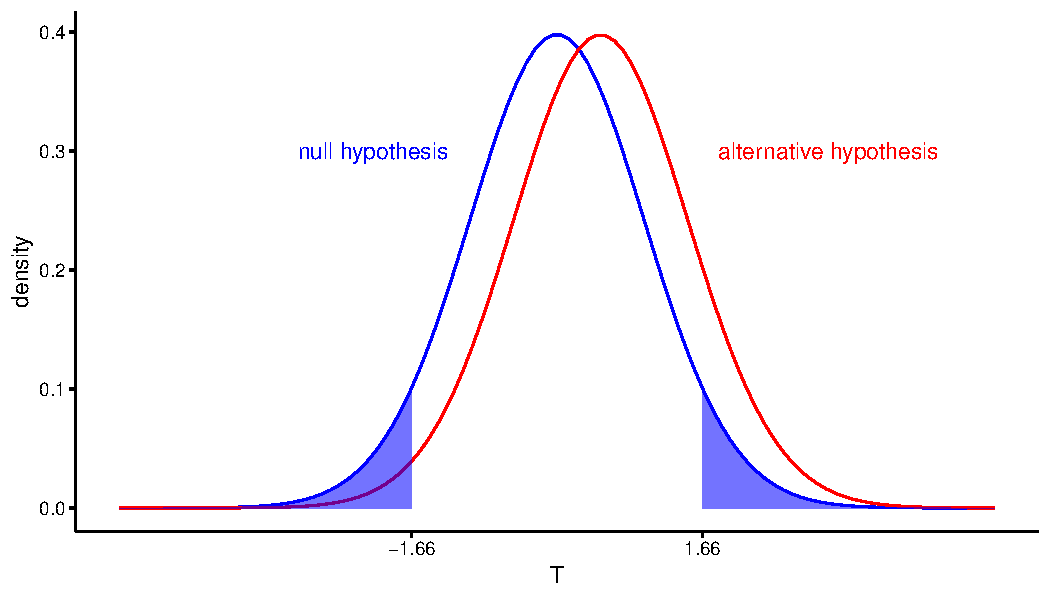
\includegraphics[width=\maxwidth]{figure/inf_20-1} 

}

\caption[Different regression lines for different values of y if x=3]{Different regression lines for different values of y if x=3.}\label{fig:inf_20}
\end{figure}


\end{knitrout}

\begin{knitrout}
\definecolor{shadecolor}{rgb}{0.969, 0.969, 0.969}\color{fgcolor}\begin{figure}

{\centering 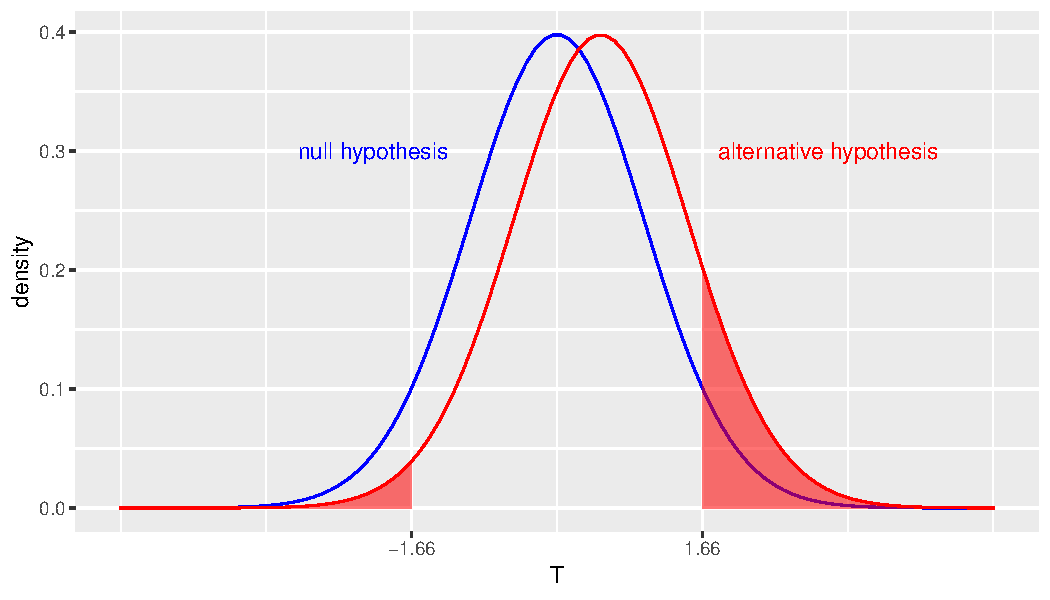
\includegraphics[width=\maxwidth]{figure/inf_21-1} 

}

\caption[Different regression lines for different values of y if x=3]{Different regression lines for different values of y if x=3.}\label{fig:inf_21}
\end{figure}


\end{knitrout}

The area that is black in Figure \ref{fig:inf_21} turns out to be $0.0906151$. This represents the probability that we find a signficant effect, \textit{if the population slope is 1}. This is actually the \textit{complement} of the probability to find a non-significant effect, \textit{if the population slope is 1}, which is $\beta$ or the probability of a type II error. Therefore, Figure \ref{fig:inf_21} represents $1- \beta$: the probability of finding a significant $p$-value, if indeed the null-hypothesis is not true. In this example, $1-\beta$ is equal to $0.0906151$, so $\beta$ is equal to its complement, $1- 0.0906151 = 0.9093849$.





In its turn, the $p$-value, as we have seen, depends on the $T$-statistic and the degrees of freedom. The degrees of freedom in turn depends on sample size. The $T$-statistic also depends on sample size, as it is partly based on the standard error.

If the alternative hypothesis is true, that is, if the population slope is not 0, then the probability of getting a $p$-value larger than 0.1, is equal to $\beta$. This is because by definition $\beta$ is the probablity of a type II error: the error that we \textit{do not reject the null-hypothesis, while the null-hypothesis is not true}. For example, suppose the population slope is 0.01. In a sample we find a slope of 1, with a $T$-statistic of 2.50 with 45 degrees of freedom. The associated $p$-value is equal to $0.016$. If $\alpha=0.01$ then we conclude that this slope of 1 is not significantly different from zero. However, since the population is actually different from 0, namely 0.01, we draw the wrong conclusion. The conditional probability\footnote{$\alpha$, $\beta$ and the $p$-value are conditional probabilities. For the distinction between a probability and a conditional probability, see \dots. In short, suppose that in the whole world, 51\% of the people are at most 17 years old. However, suppose that in the Netherlands that proportion is only 20\%. Then if we pick a random person, the probability that that person is at most 17 years old is 0.51. However, if we happen to know that the person was picked from the Dutch population, then we know better: we know that the probability has decreased to 20\%. Thus the conditional probablity that a person is under age, given that the person is Dutch, equals 0.20. The conditional probabiilty that a person is under age, given that the person is \textit{not} Dutch, equals more than 0.51.} that we find a non-significant slope (we reject the null-hypothesis), given that the population slope differs from 0 (the null-hypothesis is not true) is equal to $\beta$.


Of course we'd like to have a small $\beta$: we don't like making mistakes. So if indeed the null-hypothesis is false, we want the probability that we reject the null-hypothesis as large as possible. In order to achieve that, we need to have a $T$-value as large as possible. Since $T=b/se$, this can be achieved by having a standard error as small as possible, and this happens when our sample size is as large as possible.



%%%%%%%%%%


In later editions, Fisher explicitly contrasted the use of the p-value for statistical inference in science with the Neyman–Pearson method, which he terms "Acceptance Procedures".[19] Fisher emphasizes that while fixed levels such as 5\%, 2\%, and 1\% are convenient, the exact p-value can be used, and the strength of evidence can and will be revised with further experimentation. In contrast, decision procedures require a clear-cut decision, yielding an irreversible action, and the procedure is based on costs of error, which, he argues, are inapplicable to scientific research.

There is widespread agreement that p-values are often misused and misinterpreted.[21][22][23] One practice that has been particularly criticized is accepting the alternative hypothesis for any p-value nominally less than .05 without other supporting evidence. Although p-values are helpful in assessing how incompatible the data are with a specified statistical model, contextual factors must also be considered, such as "the design of a study, the quality of the measurements, the external evidence for the phenomenon under study, and the validity of assumptions that underlie the data analysis".[23] Another concern is that the p-value is often misunderstood as being the probability that the null hypothesis is true.[23][24] Some statisticians have proposed replacing p-values with alternative measures of evidence,[23] such as confidence intervals,[25][26] likelihood ratios,[27][28] or Bayes factors,[29][30][31] but there is heated debate on the feasibility of these alternatives.[32][33] Others have suggested to remove fixed significance thresholds and to interpret p-values as continuous indices of the strength of evidence against the null hypothesis.[34][35]
%%%%%%%%%%%%%




In 2016, the American Statistical Association published a statement on $p$-values, saying that "the widespread use of 'statistical significance' (generally interpreted as '$p \leq 0.05$') as a license for making a claim of a scientific finding (or implied truth) leads to considerable distortion of the scientific process".



\section{Relationship between $p$-value and confidence intervals}
We could have also come to the same conclusion using the 95\% confidence interval. If we find a sample slope of 1, and we know that the standard error is equal to 2, then we can find the 95\% confidence interval for the $T$-statistic (0.5) if we use a $t$-distribution with 38 degrees of freedom. From tables we can deduce that with a $t$-distribution of 38 degrees of freeedom, 2.5\% of the area is left of -2.0243942 and 2.5\% of the area is right of 2.0243942. This way we know that the confidence interval for the $T$-value is from $1  -2.0243942\times 2$ to $1 + 2.0243942\times 2$, so from $-3.0487883$ to -3.0487883.

We see that the value 0 is within this range, so 0 is a reasonable value for the population slope. From this we know that the $p$-value for the null-hypothesis is less than 5\%.


\begin{knitrout}
\definecolor{shadecolor}{rgb}{0.969, 0.969, 0.969}\color{fgcolor}\begin{figure}

{\centering 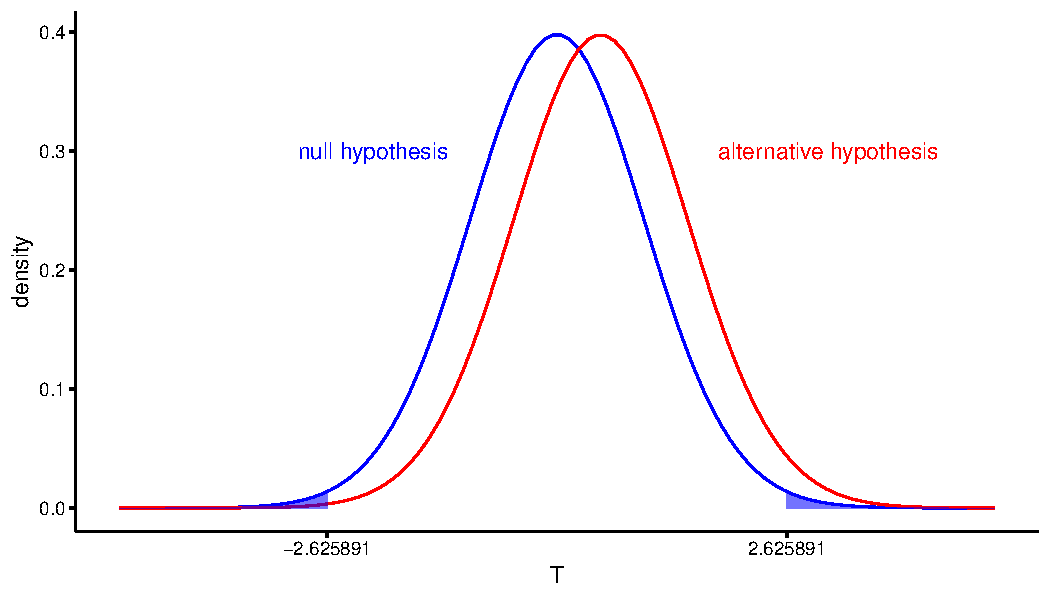
\includegraphics[width=\maxwidth]{figure/inf_22-1} 

}

\caption[Different regression lines for different values of y if x=3]{Different regression lines for different values of y if x=3.}\label{fig:inf_22}
\end{figure}


\end{knitrout}


\begin{knitrout}
\definecolor{shadecolor}{rgb}{0.969, 0.969, 0.969}\color{fgcolor}\begin{figure}

{\centering 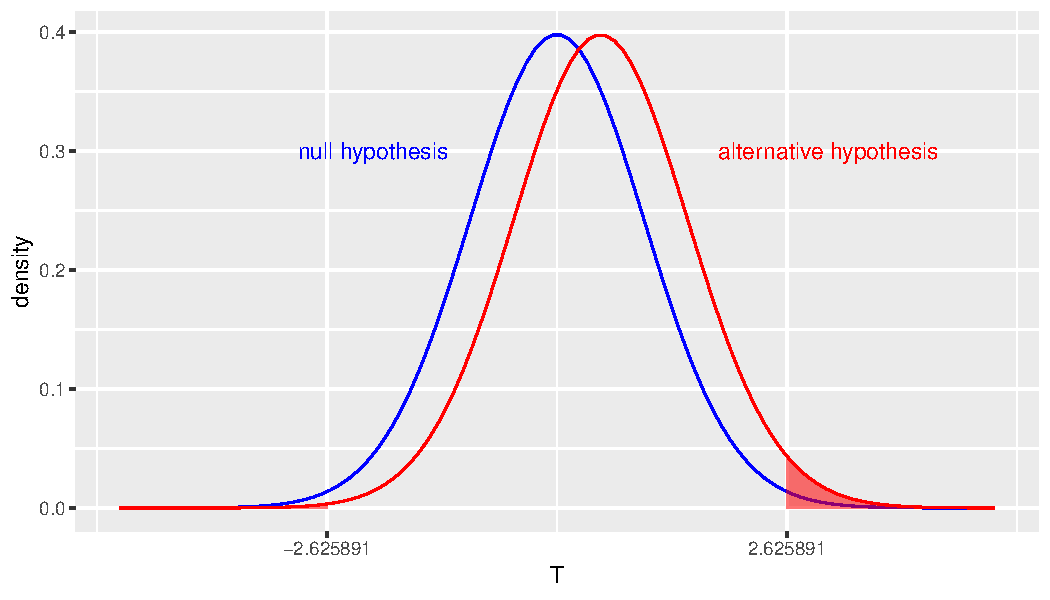
\includegraphics[width=\maxwidth]{figure/inf_23-1} 

}

\caption[Different regression lines for different values of y if x=3]{Different regression lines for different values of y if x=3.}\label{fig:inf_23}
\end{figure}


\end{knitrout}



\section{Criticism on null-hypothesis testing and $p$-values}






\section{Inference: from sample to population}


Remember, we're usually not interested in whether there is a linear relationship between x and y in a sample. The probability that the sample slope will be exactly 0 is practically zero, so the answer will be usually no.
We're usually interested in the population: is there a linear relationship between x and y in the population?

But when we think about it, it is often ridiculous to think that the population slope will be 0 exactly! Why not 0.00000111 or -0.000000008827100? Why is a slope of exactly 0 very improbable for a sample size of 200 bottles, but less improbable in the population of 80,000 bottles? Perhaps a more interesting question is how large is the population slope?

So, instead of asking research questions like Is there a linear relationship between x and y? you might ask: How large is the linear effect of x on y? Instead of a question like Is there an effect of the intervention? it might be more interesting to ask: How large is the effect of the intervention?




% knit_child('chapter_5.Rnw') % dummy variables and categorical predictors
% knit_child('chapter_6.Rnw') % moderation
% knit_child('chapter_7.Rnw') % assumptions
% knit_child('chapter_8.Rnw') % advanced topics linear models

%% contrasts en post hoc zijn nog te lastig te volgen, en zorg dat data niet 1 2 3 is, maar met betere labels, strings. niet te veel stapjes met contrast equations.

% knit_child('chapter_9.Rnw') % nonparametric alternatives linear models


\chapter{Linear mixed modelling: introduction}


\section{Fixed effects and random effects}
In the simplest form of linear modelling, we have one dependent continuous variable, one intercept and one or more independent variables. Let's look at a simple regression equation where dependent variable $y$ is predicted by an intercept $b_0$ and a linear effect of independent variable $x_1$ with regression slope parameter $b_1$, and an error term $e$, where we assume that the error term $e$ comes from a normal distribution. 


\begin{eqnarray}
y = b_0 + b_1 x_1 + e \\
e \sim N(0, \sigma^2)
\end{eqnarray}

Using this model, we know that for a person with a value of 5 for $x_1$, we expect $y$ to be equal to $b_0 + b_1 \times 5$. As another example, if $y$ is someone's IQ score, $x_1$ is someone's brain size in cubic milliliters, $b_0$ is equal to 70, and $b_1$ is equal to 0.1, we expect on the basis of this model that a person with a brain size of 1500 cubic millimeters has an IQ score of $70 + 0.01 \times 1500$, which equals 85.
\\
\\
Now, for any model the predicted values usually are not the same as the observed values. If the model predicts on the basis of my brain size that my IQ is 140, my true IQ might be in fact 130. This discrepancy is termed the residual: the observed $y$, minus the predicted $y$, or $\hat{y}$, so in this case the residual is $y - \hat{y}=130-140= -10$.
\\
\\
Here we have the model for the relationship between IQ and brain size.

\begin{eqnarray}
IQ = 70 + 0.1 \times Brainsize + e \\
e \sim N(0, \sigma^2)
\end{eqnarray}

Note that in this model, the values of 70 and 0.1 are \textit{fixed}, that is, we use the same intercept and the same slope for everyone. You use these values for any person, for Henry, Jake, Lizz, and Margaret. We therefore call these effects of intercept and slope \textit{fixed effects}, as they are all the same for all research units. In contrast, we call the $e$ term, the random error term or the residual in the regression, a \textit{random effect}. This is because the error term is \textit{different for every research unit}. We don't know the specific values of these random errors or residuals for every person, but nevertheless, we assume that they come from a distribution, in this case a normal distribution with mean 0 and an unknown variance. This unknown variance is given the symbol $\sigma^2$ 

Here are a few more examples. 

\begin{enumerate}
\item Suppose we study a number of schools, and for every school we use a simple linear regression equation to predict the number of students (dependent variable) on the basis of the number of teachers (independent variable). For every research unit (in this case: school), the intercept and the regression slope are the same (fixed effects), but the residuals are different (random effect). 

\item Suppose we study a number of students, and for every student we use a simple linear regression equation to predict the math test score on the basis of the number of hours of study the student puts in. Here, the research unit is student, and for every student, the  intercept and the regression slope are the same (fixed effects), but the residuals are different (random effect).

\item Suppose we study reaction times, and for every measure of reaction time -- a trial -- we use a simple linear regression equation to predict reaction time in milliseconds on the basis of the characteristics of the stimulus. Here, the research unit is trial, and for every trial, the intercept and the regression slope are the same (fixed effects), but the residuals are different (random effect).
\end{enumerate}

Now, what happens when we have a lot of data on students, but the students come from different schools? Suppose we want to predict average grade for every student, on the basis of the number of hours of study the student puts in. We again could use a simple linear regression equation. 

\begin{eqnarray}
y = b_0 + b_1 hourswork + e \\
e \sim N(0, \sigma^2)
\end{eqnarray}



That would be fine if all schools would be all very similar. But suppose that some schools have a lot of high scoring students, and some schools have a lot of low scoring students? Then school itself would also be a very important predictor, apart from the number of hours of study. One thing we could therefore do is to include school as a categorical predictor. We would then have to code this school variable into a number of dummy variables. The first dummy variable called $school1$ would indicate whether students are in the first school (school1=1) or not (school1=0). The second dummy variable $school2$ would indicate whether students are in the second school (school2=1) or not (school2=0), etcetera. You can then add these dummy variables to the regression equation like this:

\begin{eqnarray}
y = b_0 + b_1 hourswork + b_2 school1 + b_3 school2 + b_4 school3 + ... + e  \nonumber\\
e \sim N(0, \sigma^2)  \nonumber
\end{eqnarray}

In the output we would find a large number of effects, one for each dummy variable. For example, if the students came from 100 different schools, I would get 99 fixed effects for the 99 dummy variables. However, one could wonder whether this is very useful. As stated earlier, fixed effects are called fixed because they are the same for every unit of research, in this case every student. But working with 99 dummy variables, where students mostly score 0, this seems very much over the top. In fact, we're not even interested in these 99 effects. We're interested in the relationship between test score and hours of work, meanwhile taking into account that there are test score differences across schools. The dummy variables are only there to account for differences across schools; the prediction for one school is a little bit higher or lower than for another school, depending on how well students generally perform in each school. 
\\
\\
We could therefore try an alternative model, where we treat the school effect as $random$: we assume that every school has a different average test score, and that these averages are normally distributed. We call these average test score deviations \textit{school effects}:

\begin{eqnarray}
y = b_0 + b_1 hourswork + schooleffect + e \\
schooleffect \sim N(0, \sigma_s^2)\\
e \sim N(0, \sigma_e^2)
\end{eqnarray}

So in this equation, the intercept is fixed, that is, the intercept is the same for all observed test scores. The regression coefficient $b_1$ for the effect of hours of work is also fixed. But the schooleffect is random, since it is different for every school. The residual $e$ is also random, being different for every student. It could also be written like this:

\begin{eqnarray}
y = (b_0  + schooleffect) + b_1 hourswork + e \\
schooleffect \sim N(0, \sigma_s^2)\\
e \sim N(0, \sigma_e^2)
\end{eqnarray}


This representation emphasizes that for every school, the intercept is a little bit different: for school A the intercept might be $b_0 + 2$, and for school R the intercept might be $b_0 - 3$.

So, this equation states that every observed test score is 1) partly influenced by an intercept that is random, with a certain average $b_0$ and variance $\sigma_s^2$, that is dependent on which school students are in, 2) partly influenced by the number of hours of work, an effect that is the same no matter what school a student is in (fixed), and 3) partly influenced by unknown factors, indicated by a random residual $e$ coming from a normal distribution with variance $\sigma^2_e$.

To put it more formally: test score $y_{ij}$, that is, the test score from student $j$ in school $i$, is the sum of an effect of the school $b_0 + schooleffect_i$ (the average test score in school $i$), plus an effect of hours of work,  $b_1 \times hourswork$, and an unknown residual $e_{ij}$ (a specific residual for the test score for studuent $j$ in school $i$).

\begin{eqnarray}
y_{ij} = b_0 + schooleffect_i + b_1 hourswork + e_{ij} \\
schooleffect_i \sim N(0, \sigma_s^2)\\
e_{ij} \sim N(0, \sigma_e^2)
\end{eqnarray}

So in addition to the assumption of residuals that have a normal distribution with mean 0 and variance $\sigma_s^2$, we also have an assumption that the school averages are normally distributed, in this case with mean $b_0$ and variance $\sigma_s^2$.
\\
\\
Let's go back to the example of reaction times. Suppose in an experiment we measure reaction time in a large number of trials. We want to know whether the size of the stimulus (large/small) has an effect on reaction time. Let's also suppose that we carry out this experiment with 20 participants, where every participant is measured during 100 trials: 50 large stimuli and 50 small stimuli in random order. Now probably, some participants show generally very fast responses, and some participants show generally very slow responses. In other words, the average reaction time for the 100 trials may vary from participant to participant. This means that we can use participant as an important predictor of reaction times. To take this into account we can use the following equation:


\begin{eqnarray}
y_{ij} = b_0 + speed_i + b_1 size + e_{ij} \\
speed_i \sim N(0, \sigma_s^2)\\
e_{ij} \sim N(0, \sigma_e^2),
\end{eqnarray}

where $y_{ij}$, is the reaction time $j$ from participant $i$, $(b_0 + speed_i)$ is a random effect representing the average speed for each participant $i$ (where $b_0$ is the overall average across all participants), $b_1$ is the fixed effect of the size of the stimulus, and unknown residual $e_{ij}$ is a specific residual for the reaction time for trial $j$ of participant $i$.
\\
\\
The reason for introducing random effects is that when your observed data are clustered, for instance student scores clustered within schools, or trial response times are clustered within participants, you violate the assumption of independence: two reaction times from the same person are more similar than two reaction times from different persons. Two test scores from students from the same school may be more similar than two scores from students in different schools. When this is the case, when data are clustered, it is very important to take this into account. When the assumption of independence is violated, you are making wrong inference if you only use a simple linear model. With clustered data, it is therefore necessary to work with an extension of the linear model, the so-called linear mixed model. The above models for test scores across different schools and reaction times across different participants, are examples of \textit{linear mixed models}. The term \textit{mixed} comes from the fact that the models contain a mix of both fixed and random effects. 
\\
\\
If you have clustered data, you should take this clustering into account, either by using the grouping variable as a qualitative predictor (using a number of dummy variables) or by using a linear mixed model. As a rule of thumb: if you have fewer than 10 groups, consider dummy variables; if you have 10 or more groups, consider a linear mixed model. Use a linear mixed model if the assumption of normally distributed group differences is tenable. Use dummy variables if you are actually interested in the size of group differences.
\\
\\
Below, we will start with a very simple example of linear mixed model, one that we use for a simple pre-post intervention design.



\section{Pre-post intervention design}


Imagine a study where we hope to show that aspirin helps reduce headache. For 100 patients we ask to rate the severity of their headache before they use aspirin (on a scale from 1 - 100), and to rate the severity again 3 hours after taking 500 mg of aspirin. These patients were randomly selected among people who read the NY Times and suffer from regular headaches. So here we have clustered data: we have 100 patients, and for each patient we have two scores, one before (pre) and one after (post) the intervention of taking aspirin. Of course headaches differ from person to person, so we might have to take into account that some patients have a higher average level of headache than other patients. Now, the data could be represented in different ways, but suppose we have the following data matrix (showing only the first 5 patients):
 \\
 \\
 \begin{tabular}{lrr}
 patient & pre & post \\ \hline
 001 & 55 & 45 \\
 002 & 63 & 50 \\
 003 & 66 & 56 \\
 004 & 50 & 37 \\
 005 & 63 & 50 \\
 \dots & \dots & \dots \\
 \end{tabular}
\\
\\
What we observe here is that the severity seems generally lower after the intervention than before the intervention. But you may also notice that the severity of the headache also varies across patients: some have generally high scores (for instance patient 003), and some have generally low scores (for example patient 001). Therefore, the headache scores seem to be clustered, violating the assumption of independence. We can quantify this clustering by computing a correlation between the pre-intervention scores and the post-intervention scores. Here it appears that there is a strong positive correlation, indicating that the higher the pain score before the intervention, the higher the pain score after the intervention. 
\\
\\

There is an alternative way of representing the same data. Let's look at the same data in a new format:
\begin{knitrout}
\definecolor{shadecolor}{rgb}{0.969, 0.969, 0.969}\color{fgcolor}
\begin{tabular}{r|r|r}
\hline
patient & measure & headache\\
\hline
1 & 1 & 55\\
\hline
1 & 2 & 45\\
\hline
2 & 1 & 63\\
\hline
2 & 2 & 50\\
\hline
3 & 1 & 66\\
\hline
3 & 2 & 56\\
\hline
4 & 1 & 50\\
\hline
4 & 2 & 37\\
\hline
5 & 1 & 63\\
\hline
5 & 2 & 50\\
\hline
\end{tabular}


\end{knitrout}
%  \\
%  \\
%  \begin{tabular}{lrr}
%  patient & intervention & severity \\ \hline
%  001 & pre & 80 \\
%  001 & post & 65 \\
%  002 & pre & 34 \\
%  002 & post & 25 \\
%  003 & pre & 23 \\
%  003 & pre & 15 \\
%  004 & post & 90 \\
%  004 & pre & 70 \\
%  005 & post & 23 \\
%  005 & pre & 13 \\
%  \dots & \dots & \dots \\
%  \end{tabular}
% \\
% \\
Here we acknowledge that there is really only one dependent measure: headache severity. The other two variables indicate that this variable varies across both patients and time point (pre intervention and post intervention). Here we might consider applying a simple linear regression model, using severity as the dependent variable and \textbf{measure} (1st or 2nd) as a qualitative predictor (using a dummy variable). However, since we know that there is a correlation between the pre and post severity measures, we know that measures systematically vary across patients: some score high on average and some score low on average. Therefore we have to run a linear \textit{mixed} model, including not only the fixed effect of \textbf{measure} but also a random effect for each patient. Since we are really interested in the effect of the intervention, that is, we want to know how large the effect of aspirin is, we use a fixed effect for the time effect (the variable \textbf{measure}). For the patient effect, because there are so many patients (100) and we're really not interested in all of these individual differences, we use a random effect. This means that we only assume there is a normal distribution for all of the patient differences. So we get the following equation:


\begin{eqnarray}
y_{ij} = b_0 + patient_i + b_1 measure + e_{ij} \\
patient_i \sim N(0, \sigma_p^2)\\
e_{ij} \sim N(0, \sigma_e^2)
\end{eqnarray}

$y_{ij}$ is the $j$th headache severity score (first or second) for patient $i$, $(b_0 + patient_i)$ is the average headache for patient $i$, \textit{measure} is a dummy variable for which measure (first or second), and $b_1$ is the effect of the intervention (by how much the severity changes from pre to post). We assume that the average pain level for each patient shows a normal distribution with average $b_0$ and variance $\sigma^2_p$. And of course we assume that the residuals show a normal distribution.
\\
\\
This analysis can be done with the following SPSS syntax, treating time as a qualitative variable (using BY) for which SPSS will create a dummy variable automatically. 


\begin{verbatim}
MIXED headache  BY measure
  /FIXED=measure
  /PRINT=DESCRIPTIVES  SOLUTION
  /RANDOM=intercept | SUBJECT(patient) COVTYPE(VC).
\end{verbatim}


\begin{figure}[h]
    \begin{center}
       \includegraphics[scale=0.8, trim={0cm 20cm 0cm 0cm} ]{/Users/stephanievandenberg/Dropbox/Statistiek_Onderwijs/Data" "Analysis/spss" "examples" "linear" "mixed" "model/prepost/prepost.pdf}
    \end{center}
\end{figure}

The most interesting output is given here. We're mostly interested in the fixed effect of the intervention: does aspirin reduce headache? After an F-test, we see the linear model coefficients, with an intercept of around 49 and a positive effect of the intervention dummy variable, around $+10$. We see that the dummy variable was coded 0 for the second measure and 1 for first meausure. So, for our dependent variable headache, we see that the expected headache severity for the observations with a 0 for the dummy variable (that is, measure 2, which is \textit{after} taking aspirin), is equal to $49 + (10) \times 0 = 49$. Similarly, we see that the expected headache severity for the observations with a 1 for the dummy variable (that is, \textit{before} taking aspirin), is equal to $49 + (10) \times 1 = 49 + 10 = 59$. So, average pain severity is 10 points higher before the intervention than after the intervention. Whether this difference is significant is indicated by a $t$-test. We see here that the average headache severity after taking an aspirin is significantly different from the average headache severity before taking an aspirin, $t(99) = 25.46, p < 0.01$. The degrees of freedom are taken from the Test of Fixed Effects table with the $F$-statistics. Alternatively we can write 

\begin{quote}
{The average headache severity after taking an aspirin is significantly different from the average headache severity before taking an aspirin, $F(1,99) = 648.28, p < 0.01$}\end{quote}


We might therefore carefully conclude that aspirin reduces headache in the population of NY Times readers with headache problems, where the reduction is around 10 points on a 1...100 scale (95\% CI: 9.55 -- 11.17). 
\\
\\
Now, this looks like reporting the output of a regular linear model, but of course it isn't. We also have some extra output, about the random effect of patient. We assumed that the individual differences in headache severity in the 100 patients came from a normal distribution. How large are these individual differences actually? This can be gleaned from the Covariance Parameters part of the SPSS output. We there see two random effects: the one for the residuals and one for the patients. The intercept seems to vary with a variance of 27, which is equivalent to a standard deviation of $\sqrt{27}$ which is around 5.2. What does that mean exactly? Well let's look at the equation again and fill in the numbers:

\begin{eqnarray}
y_{ij} = b_0 + patient_i + b_1 measure + e_{ij} \\
y_{ij} = 49 + patient_i + 10 measure + e_{ij} \\
patient_i \sim N(0, 27)\\
e_{ij} \sim N(0, 8)
\end{eqnarray}

Since measure is coded 0 for the headache level after the intervention, we conclude that the average pain level after taking aspirin is 49. However, not everybody's pain level after taking aspirin is 49: people show variance. The pain level after aspirin varies with a variance of 27, which is equavalent to a standard deviation of arond 5.2. Figure below shows how much this variance actually is. It depicts a normal distribution with mean 49 and a standard deviation of 5.2.


\begin{knitrout}
\definecolor{shadecolor}{rgb}{0.969, 0.969, 0.969}\color{fgcolor}

{\centering 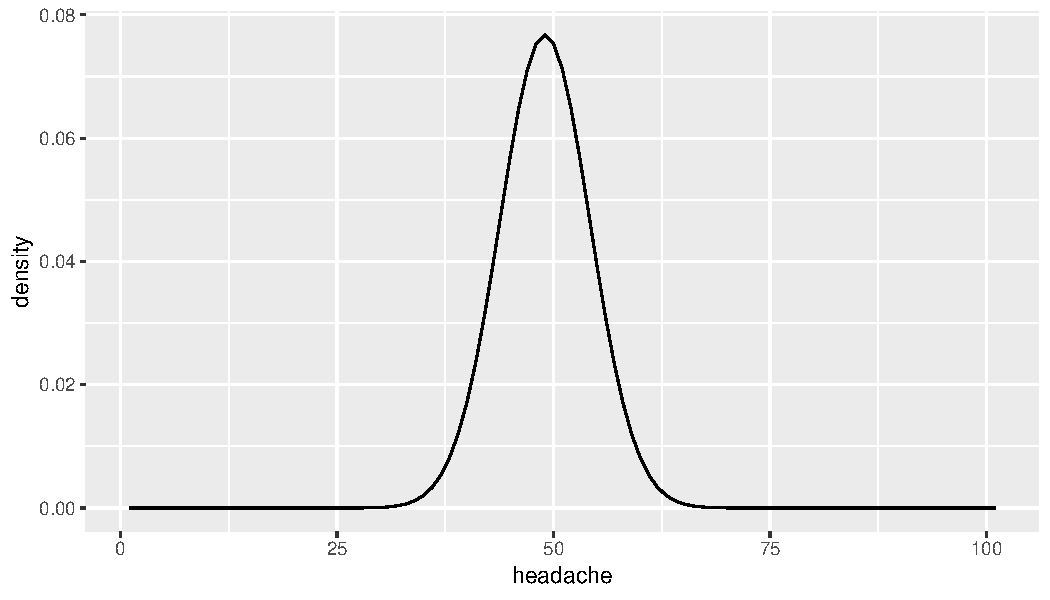
\includegraphics[width=\maxwidth]{figure/resultsprepost1-1} 

}



\end{knitrout}

So \textit{after} taking aspirin, most patients show headache levels between 30 and 60. More specificially, if we would take the middle 95\% by using plus or minus twice the standard deviation, we can estimate that 95\% of the patients shows levels between $49 - 2 \times 5.2 = 38.6$ and $49 + 2 \times 5.2 = 59.4$
\\
\\
Now let's look at the levels \textit{before} taking aspirin. The average headache leves is equal to $49 + 10 = 59$. So 95\% of the patients shows headache levels between $59 - 2 \times 5.2 = 48.6$ and $59 + 2 \times 5.2 = 49.4$ before taking aspirin. 
\\
\\
Together these results can be graphically explained in the plot below:
\begin{knitrout}
\definecolor{shadecolor}{rgb}{0.969, 0.969, 0.969}\color{fgcolor}

{\centering 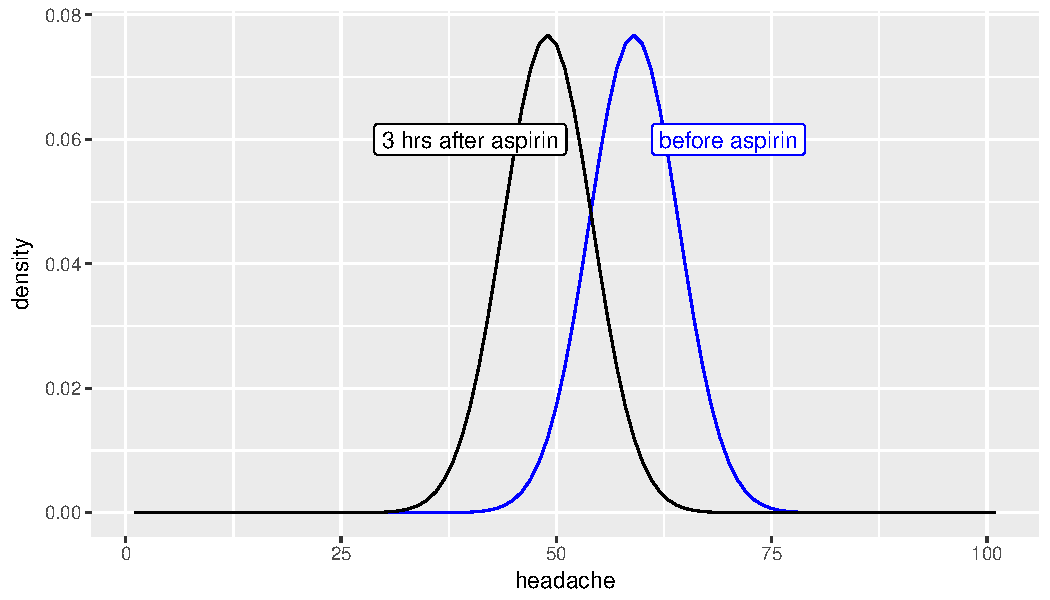
\includegraphics[width=\maxwidth]{figure/resultsanalysisprepost2-1} 

}



\end{knitrout}


In this plot you see there is variability in headache levels before taking aspirin, and there is variation in headache levels after taking aspirin. We also see that these distributions have the same spread (variance): in the model we assume that the variability in headache before aspirin is equal to the variability after aspirin. The distributions are equal, except for a horizontal shift: the distribution for heachache after aspirin is the same as the distribution before apsirin, except for a shift to the left of about 10 points. This is of course the effect of aspirin in the model, the $b_1$ parameter in our model above. 
\\
\\
The fact that the two distributions before and after aspirin show the same spread (variance) was an inherent assumption in our model: we only have one random effect for patient in our output. If the assumption of equal variance (homoscedasticity) is not tenable, then one should consider other linear mixed models. But this is beyond the scope of this chapter. The assumption can be checked by plotting the residuals, using differnt colours for residuals from before taking aspirin and for residuals from after taking aspirin. 



\subsection{Exercises}

Suppose an intervention study looked at the effect of therapy on depression levels. A random sample of patients were measured before and after the therapy. Given the following equation, based on output of the statistical software package R. The dummy variable \textit{measure} was coded 0 for before therapy and 1 for after therapy.




\begin{figure}[h]
    \begin{center}
       \includegraphics[scale=0.8, trim={0cm 20cm 0cm 0cm}]{/Users/stephanievandenberg/Dropbox/Statistiek_Onderwijs/Data" "Analysis/spss" "examples" "linear" "mixed" "model/prepost/prepostdepression.pdf}
    \end{center}
\end{figure}


Look at the output below. You see information about random effects and you see information about fixed effects. 

\begin{itemize}
\item 1. What is the intercept of the model?\\
\item 2. What is the slope coefficent for the measure variable?\\
\item 3. What is the variance of the residuals? What is the standard deviation?\\
\item 4. What is the variance of the individual differences among patients? What is the standard deviation?\\
\item 5. Fill in the values in the linear mixed model below:

\begin{eqnarray}
depression_{ij} = \dots + patient_i + \dots \times measure + e_{ij} \\
patient_i \sim N(0, \sigma_p^2 = \dots)\\
e_{ij} \sim N(0, \sigma_e^2 = \dots)
\end{eqnarray}


\item 6. what can you say about the average depression level before therapy? \\
\item 7. what can you say about the average depression level after therapy?\\
\item 8. How much variance in depression level before therapy does this model predict? What is the standard deviation? \\
\item 9. Between what values do depression levels before therapy in the middle 95\% of patients show?\\
\item 10. How much variance in depression level after therapy does this model predict? What is the standard deviation? \\
\item 11. Between what values do depression levels after therapy in the middle 95\% of patients show?\\
\item 12. Does therapy help to alleviate depression in patients? You may use an approximation to construct a confidence interval.

\item 13. A researcher has two groups of patients: one group receives medicine and one group receives therapy. The null-hypothesis is that depression levels after medicine are as high as depression levels after therapy. Do we analyse these data with an ordinary linear model, or with a linear mixed model? Explain your answer.

\item 14. A researcher studies one group of students: they first get lectures from teacher A and then they get lectures from teacher B. The null-hypothesis is that the average teacher evaluation for teacher A is the same as the average teacher evaluation for teacher B. Do we analyse these data with an ordinary linear model, or with a linear mixed model? Explain your answer. 


\item 15. For a study to the effect of light on mood, we have data on 100 teachers They were asked to rate their mood on a cloudy day and asked to rate their mood on a sunny day. We have the variable \textbf{mood}, the dummy variable \textbf{sunny} and we want to include a random effect for \textbf{teacher} From the three syntaxes below, choose the one that is most suitable for your analysis and fill in the blanks.


\begin{verbatim}
MIXED ...  WITH ...
  /FIXED=...
  /PRINT=DESCRIPTIVES  SOLUTION
  /RANDOM=intercept | SUBJECT(...) COVTYPE(VC).
\end{verbatim}


\begin{verbatim}
UNIANOVA ... WITH ... 
/ design = ...
/ print = parameter.
\end{verbatim}


\begin{verbatim}
UNIANOVA ... BY ... 
/ design = ...
/ print = parameter.
\end{verbatim}


\item 16. A researcher wants to know whether students in green classrooms (colour = 1) perform better than students in yellow classrooms (colour = 2). The following data were collected (showing only a part):

\begin{knitrout}
\definecolor{shadecolor}{rgb}{0.969, 0.969, 0.969}\color{fgcolor}
\begin{tabular}{r|r|r}
\hline
student & colour & performance\\
\hline
1 & 1 & 6.79\\
\hline
2 & 2 & 8.28\\
\hline
3 & 1 & 9.08\\
\hline
4 & 2 & 5.65\\
\hline
5 & 1 & 8.43\\
\hline
6 & 2 & 8.51\\
\hline
7 & 1 & 7.43\\
\hline
8 & 2 & 7.45\\
\hline
9 & 1 & 7.44\\
\hline
10 & 2 & 7.11\\
\hline
\end{tabular}


\end{knitrout}

Would you use an ordinary linear model or a linear mixed model to analyze these data? Explain your answer.

\item 17. A researcher wants to know whether students in dark classrooms (brightness = 0) perform better than students in bright classrooms (brightness = 1). The following data were collected (showing only a part):


\begin{knitrout}
\definecolor{shadecolor}{rgb}{0.969, 0.969, 0.969}\color{fgcolor}
\begin{tabular}{r|r|r}
\hline
student & brightness & performance\\
\hline
1 & 0 & 8.66\\
\hline
1 & 1 & 5.95\\
\hline
2 & 0 & 6.50\\
\hline
2 & 1 & 9.47\\
\hline
3 & 0 & 9.46\\
\hline
3 & 1 & 8.14\\
\hline
4 & 0 & 8.21\\
\hline
4 & 1 & 4.96\\
\hline
5 & 0 & 7.51\\
\hline
5 & 1 & 6.91\\
\hline
\end{tabular}


\end{knitrout}

Would you use an ordinary linear model or a linear mixed model to analyze these data? Explain your answer.



\item 18.
A landscaper believes that people get more creative once the environment becomes greener. She measures creativity before and after the introduction of new trees around the office building in a random sample of employees. Because creativity can also be influenced by the weather she also uses a dummy variable \textbf{sunny} to correct for these effects. Whether creativity is meassured before or after the introduction of the trees is indicated by the variable \textbf{green} that is coded green=1 for after the introduction and green=0 for before the introduction. The model that she therefore runs in SPSS is the following:

\begin{verbatim}
MIXED creativity  WITH green sunny
  /FIXED= green sunny
  /PRINT=DESCRIPTIVES  SOLUTION
  /RANDOM=intercept | SUBJECT(employee) COVTYPE(VC).
\end{verbatim}

We get the following output: 

\begin{figure}[h]
    \begin{center}
       \includegraphics[scale=0.8, trim={0cm 20cm 0cm 0cm}]{/Users/stephanievandenberg/Dropbox/Statistiek_Onderwijs/Data" "Analysis/spss" "examples" "linear" "mixed" "model/prepost/prepostcreativity.pdf}
    \end{center}
\end{figure}

Write a short paragraph describing these results and the conclusions in APA format.


\end{itemize}


\subsubsection{Answers:}

\begin{itemize}

\item Ad1: 10.57 \\
\item Ad2: -2.28 \\
\item Ad3: 8.31,2.88 \\
\item Ad4: 1.79,1.34 \\

\item Ad5:
\begin{eqnarray}
depression_{ij} = 10.57 + patient_i + (-2.28) \times measure + e_{ij} \\
patient_i \sim N(0, \sigma_p^2 = 1.79)\\
e_{ij} \sim N(0, \sigma_e^2 = 8.31)
\end{eqnarray}




\item Ad 6: 10.57\\
\item Ad 7: 10.57 + -2.28  = 8.29\\
% Ad 8: SD = 1.34, variance is 1.34^2= 1.80$. \\
\item Ad 8: 1.79, 1.34 \\

\item Ad 9: $10.57 \pm 2 \times 1.34 = {7.89, 13.25}$\\

\item Ad 10: 1.79, 1.34 \\

\item Ad 11: $(10.57 -2.28)  \pm  2 \times 1.34 = {5.61, 10.79 }   $\\

\item Ad 12: For the effect of therapy (the measure variable), we see a $b$-value of -2.28 with a standard error of 0.407773, so if we use the +/-2 rule to compute a 95\% confidence interval, we get $[ -2.28 - 2\times 0.41 , -2.28 + 2\times 0.41]  = [ -3.1 ,  -1.46]$. The 95\% interval does NOT contain the value 0 so we can reject the null-hypothesis that the effect of therapy is zero. Therefore, we conclude that therapy has an influence on depression. In this case we saw a decrease in depression levels after therapy.

\item Ad 13: Two groups of patients are studied, and for each patient we have only one measure. Because we only have one measure for each unit of observation we conduct an ordinary linear model.

\item Ad 14: One group of students is studied, and for each student we have two evaluations: one for teacher A and one for teacher B. Because we have more than one measure for each unit of observation, we have to use a linear mixed model. 

\item Ad15: 

\begin{verbatim}
MIXED mood  WITH sunny
  /FIXED=sunny
  /PRINT=DESCRIPTIVES  SOLUTION
  /RANDOM=intercept | SUBJECT(teacher) COVTYPE(VC).
\end{verbatim}

\item Ad16: it seems as if each student was only measured once, there is no clustering, so we can use an ordinary linear model.

\item Ad17: it seems as if each student was measured twice, in both dark and bright conditions, so we use a linear mixed model to account for clustering.

\item Ad18: 
\begin{quotation}

A linear mixed model was run to test the effect of green surroundings on creativity. The analysis was corrected for the effects of weather (sunny or not sunny) and random effects for employees. The results showed a significant but negative effect of the introduction of trees on creativity: creativity was on average 4.5 points lower after the introduction, $t(98)=-10.47, p < 0.001$. This effect was present over and above the effect of the weather which by itself had also an effect, where creativity was 1.28 points lower on sunny days than on not cloudy days, $t(98)=-2.32, p=0.02$. The variance not explained by weather and greenness was largely explained by individual differences in creativity among employees, with an intraclass correlation of $\frac{23.7}{23.7+9.2}= 0.72$. We conclude that the introduction of trees has a negative influence on creativity in the employees that worked in the building studied in this research. 

\end{quotation}

\end{itemize}



\section{Pre-mid-post intervention design}


In many intervention studies, one has more than two measurement moments. For instance, you'd like to know if there is not only a short term effect of aspirin, but also a long-term effect. Suppose that the study mentioned in the previous section on headache among NY Times readers was extended by asking patients not only to rate their headache before aspirin and 3 hours after intake, but also 24 hours after intake. In this case our data could look like this:

\begin{knitrout}
\definecolor{shadecolor}{rgb}{0.969, 0.969, 0.969}\color{fgcolor}
\begin{tabular}{r|r|r|r}
\hline
patient & measure1 & measure2 & measure3\\
\hline
1 & 52 & 45 & 47\\
\hline
2 & 59 & 50 & 55\\
\hline
3 & 65 & 56 & 58\\
\hline
4 & 51 & 37 & 42\\
\hline
5 & 62 & 50 & 55\\
\hline
6 & 61 & 53 & 57\\
\hline
7 & 56 & 44 & 55\\
\hline
8 & 62 & 48 & 53\\
\hline
9 & 56 & 48 & 49\\
\hline
10 & 58 & 45 & 44\\
\hline
\end{tabular}


\end{knitrout}

So for each patient we have three measures: pre, post1 and post2. To see if there is some significant clustering, it is no longer possible to study this by computing a single correlation. We could however compute 3 different correlations: pre-post1, pre-post2, and post1-post2, but this is rather tedious, and moreover does not give us a single measure of the extent of clustering of the data. But there is an alternative: one could compute not a Pearson correlation, but an \textit{intraclass correlation} (ICC). To do this, we need to bring the data again into a regression type format, like this (we call this \textit{long format}, as opposed to \textit{wide format}):

\begin{knitrout}
\definecolor{shadecolor}{rgb}{0.969, 0.969, 0.969}\color{fgcolor}
\begin{tabular}{r|r|r}
\hline
patient & measure & headache\\
\hline
1 & 1 & 52\\
\hline
1 & 2 & 45\\
\hline
1 & 3 & 47\\
\hline
2 & 1 & 59\\
\hline
2 & 2 & 50\\
\hline
2 & 3 & 55\\
\hline
3 & 1 & 65\\
\hline
3 & 2 & 56\\
\hline
3 & 3 & 58\\
\hline
4 & 1 & 51\\
\hline
\end{tabular}


\end{knitrout}

We can perform an analysis using a MIXED analysis in SPSS:

\begin{verbatim}

MIXED headache BY measure
  /FIXED=measure
  /PRINT=DESCRIPTIVES  SOLUTION
  /RANDOM=intercept | SUBJECT(patient) COVTYPE(VC).
\end{verbatim}

The output is given below:

\begin{figure}[h]
    \begin{center}
       \includegraphics[scale=0.8, trim={0cm 20cm 0cm 0cm} ]{/Users/stephanievandenberg/Dropbox/Statistiek_Onderwijs/Data" "Analysis/spss" "examples" "linear" "mixed" "model/premidpost/premidpostaspirin.pdf}
    \end{center}
\end{figure}


In the output we see the fixed effects of two automatically created dummy variables \textbf{measure=1} and \textbf{measure=2}, and the intercept. We also see the variances of the random effects: the variance of the residuals and the variance of the random effects for each patient.

From this output, we can plug in the values into the equation:


\begin{eqnarray}
headache_{ij} = 51 + patient_i +7.5 \times measure1 - 2.4 \times measure2 + e_{ij} \nonumber\\
patient_i \sim N(0, 28.3)\nonumber\\
e_{ij} \sim N(0, 8.5)\nonumber
\end{eqnarray}

Based on this equation, the expected headache severity score in the population 24 hours after aspirin intake is 51 (the third measure is the reference group). Dummy variable \textbf{measure=1} is coded 1 for the measurements before taking aspirin. Therefore, the expected headache score before aspirin intake is equal to $51+7.5 = 58.5$. Dummy variable \textbf{measure=2} was coded 1 for the measurements 3 hours after aspirin intake. Therefore, the expected headache score 3 hours after aspirin intake is equal to $51 - 2.4 = 48.6$. In sum, in this sample we see that the average headache level decreases directly after aspirin intake from 58.5 to 48.6, but then increases again to 51. 
\\
\\
There was quite some variation in individual headache levels: the variance is equal to 28.3, so the standard deviation (its square root) is equal to about 5.3. Therefore, if we look at roughly 95\% of the sample, we see that prior to taking aspirin, the scores vary between $58.5 -2\times 5.3 = 47.9$ and $58.5 + 2 \times 5.3 = 69.1$. For the short-term effect of aspirin after 3 hours, we see that roughly 95\% of the scores lie between $48.6 -2\times 5.3 = 38.0$ and $48.6 + 2 \times 5.3 = 59.2$. The normal distributions, predicted by this model, are depicted in the figure below:


\begin{knitrout}
\definecolor{shadecolor}{rgb}{0.969, 0.969, 0.969}\color{fgcolor}

{\centering 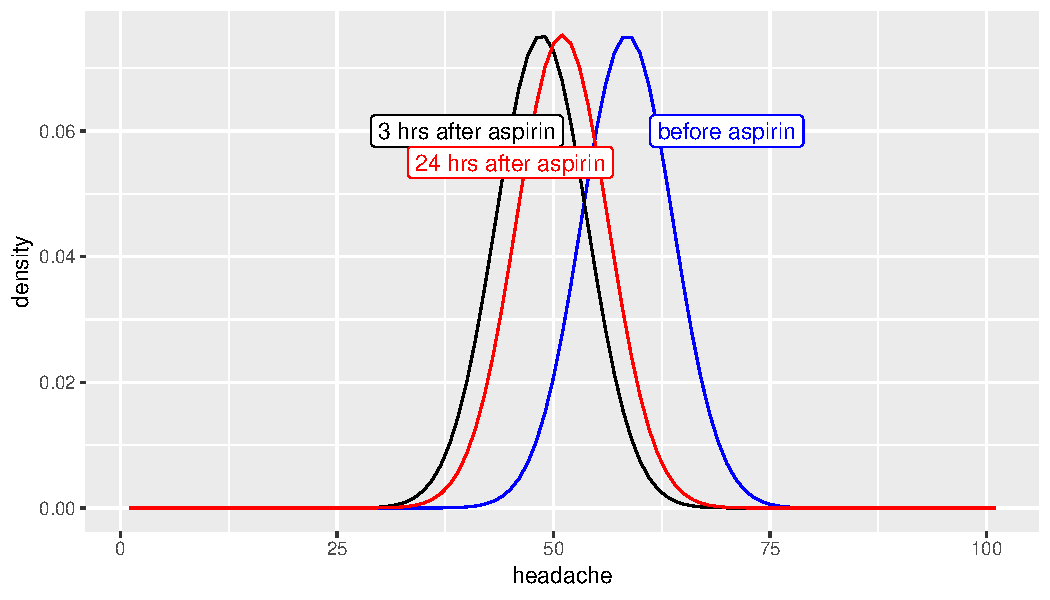
\includegraphics[width=\maxwidth]{figure/analysispremidpost3-1} 

}



\end{knitrout}



So, are these distributions significantly different, in other words, do the means differ significantly before aspirin, 3hrs after aspirin and 24 hrs after aspirin? The answer is yes, because the $F$-test on the group means in the SPSS output is significant. Note the degrees of freedom: 2, because we compare 3 groups of data, so we need two dummy variables. Thus we report that aspirin has an effect on headache levels in NY Times readers, $F(2, 198)=309.58, p<0.001$.

If one has specific hypotheses regarding short-term and long-term effects, one could perform a planned contrast analysis, comparing the first measure with the second measure, and the first measure with the third measure. If one is just interested in whether aspirin has an effect on headache, then the $F$-test should suffice. If apart from this general effect one wishes to explore whether there are significant differences between the three groups of data, without any prior research hypothesis about this, then one could perform a post hoc analysis of the three means. See the relevant chapter on how to perform planned comparisons and post hoc tests.
\\
\\
Now recall that we mentioned an intraclass correlation, or ICC. An intraclass correlation indicates how much clustering there is within the groups, in this case, clustering of headache scores within NY Times readers. How much are the three scores alike that come from the same patient? This correlation can be computed on the basis of the SPSS output, using the following formula:

\begin{eqnarray}
ICC = \frac{\sigma^2_{patient} } {\sigma^2_{patient} +\sigma^2_e }   
\end{eqnarray}

Here, the variance of the \textbf{patient} random effects is equal to 28.3, and the variance of the residuals $e$ is equal to 8.5, so the intraclass correlation for the headache severity scores is equal to 
\begin{eqnarray}
ICC = \frac{28.3} {28.3 + 8.5 } =  0.80
\end{eqnarray}

As this correlation is quite higher than 0, there seems to be quite a lot of clustering. Therefore it's a good thing that we used random effects for the individual differences in headache scores among NY Times readers. Had this correlation been 0 or very close to 0, however, then it would not have mattered to include these random effects. In that case, we might as well use an ordinary linear model, using the UNIANOVA syntax for example. Note from the formula that the correlation becomes 0 when the variance of the random effects for patients is 0.
\\
\\


\subsection{Exercises}

Suppose you let a sample of students do a math test in three different rooms: one with yellow walls, one with red walls and one with blue walls. All students do the math test three times, once in every room. The data are as follows:
\\
 \\
 \begin{tabular}{lrr}
 student & colour & score \\ \hline
 001 & yellow & 60 \\
 001 & red & 66 \\
 001 & blue & 60 \\
 002 & yellow & 24 \\
 002 & red & 15 \\
 002 & blue & 30 \\
 003 & yellow & 90 \\
 003 & red & 90 \\
 003 & blue & 89 \\
 004 & yellow & 10 \\
 004 & red & 20 \\
 004 & blue & 15 \\
 005 & yellow & 23 \\
 005 & red & 13 \\
 005 & blue & 18 \\
 \dots & \dots & \dots \\
 \end{tabular}
\\
\\

\begin{itemize}
\item 1. If you want to test the hypothesis that the colour of the walls do not affect math test scores, and at the same time you want to take into account that some students are generally better at math than others, what would the SPSS syntax be? \\
\item 2. In the output that would result from that syntax from question 1, would you look at a $t$-test or or an $F$-test? Explain your answer.
\item 3. How many degrees of freedom would you see for the denominator?\\
\item 4. Suppose you see this in the output for this colour experiment. How important are the individual difference in math performance in the population of students? Can you quantify the amount of clustering?



\begin{figure}[h]
    \begin{center}
       \includegraphics[scale=0.5]{/Users/stephanievandenberg/Dropbox/Statistiek_Onderwijs/Data" "Analysis/spss" "examples" "mixed" "linear" "model/pre-mid-post" "design/exercise2_correlation.png}
    \end{center}
\end{figure}

\end{itemize}


Answers:
\begin{itemize}
\item 1.
\\
\begin{verbatim}
MIXED score BY colour
  /FIXED=colour
  /PRINT=DESCRIPTIVES  SOLUTION
  /RANDOM=intercept | SUBJECT(student) COVTYPE(VC).
\end{verbatim}

\item 2. $F$-test. There will be two dummy variable and I want to know if the effects of both of these are significantly different from 0. The $t$-tests  give me only information about the dummy variables separately. \\
\item 3. 2, because there are 3 different colours, which can be represented by 2 dummy-variables. \\
\item 4. In the table with the data you generally see that students who score high in one room also score high in another room (for instance, students 001 and 003). Students who score low in one room also score low in another room (for instance students 002, 004 and 005). This clustering can be quantified using an intraclass correlation, in this case equal to $\frac{228}{228+270}=0.46$. 
\end{itemize}


\section{Pre-mid-post intervention design: linear effects}
In the previous section, we've looked at \textit{qualitative} variables: \textbf{measure} (pre intervention, 3 hours after, and 24 hours after), or \textbf{colour} (yellow, red, and blue rooms). We can use the same type of analysis for \textit{quantitative} variables. In fact, we could have used a linear effect for time in the headache example: using time of measurement as a variable. Let's look at the headache data again. But now we've created a new variable \textbf{time} that is based on the measure \textbf{variable}: all first measurements are coded as \textbf{time}=0, all second measurements after 3 hours are coded as \textbf{time}=3, and all third measurements after 24 hours are coded as \textbf{time}=24.

\begin{knitrout}
\definecolor{shadecolor}{rgb}{0.969, 0.969, 0.969}\color{fgcolor}
\begin{tabular}{r|r|r|r}
\hline
patient & measure & headache & time\\
\hline
1 & 1 & 52 & 0\\
\hline
1 & 2 & 45 & 3\\
\hline
1 & 3 & 47 & 24\\
\hline
2 & 1 & 59 & 0\\
\hline
2 & 2 & 50 & 3\\
\hline
2 & 3 & 55 & 24\\
\hline
3 & 1 & 65 & 0\\
\hline
3 & 2 & 56 & 3\\
\hline
3 & 3 & 58 & 24\\
\hline
4 & 1 & 51 & 0\\
\hline
\end{tabular}


\end{knitrout}
 
 
Instead of using a qualitative variable intervention, with three levels, we now use a quantitative variable, time, indicating the number of hours that have elapsed after aspirin intake. At point 0 hours, we measure headache severity, and patients take an aspirin. Next we measure headache after 3 hours and 24 hours. Above, we wanted to know if there were differences in average headache between before intake and 3hrs and 24 hrs after intake. Another question we might ask ourselves: is there a \textit{linear} reduction in headache severity after taking aspirin?

For this we can do a linear regression type of analysis. We want to take into account individual differences in headache severity levels among patients, so we perform a MIXED analysis in SPSS, using the following syntax, replacing the key word BY with WITH, and the variable \textbf{measure} by \textbf{time}:

\begin{verbatim}
MIXED headache WITH time
  /FIXED=time
  /PRINT=DESCRIPTIVES  SOLUTION
  /RANDOM=intercept | SUBJECT(patient) COVTYPE(VC).
\end{verbatim}


Below we see the corresponding output:

\begin{figure}[h]
    \begin{center}
       \includegraphics[scale=0.8, trim={0cm 20cm 0cm 0cm} ]{/Users/stephanievandenberg/Dropbox/Statistiek_Onderwijs/Data" "Analysis/spss" "examples" "linear" "mixed" "model/premidpost/premidpostaspirinlinear.pdf}
    \end{center}
\end{figure}


Based on the output, we see that the model for our data is equivalent to


\begin{eqnarray}
headache_{ij} = 54 + patient_i - 0.16 \times time + e_{ij} \\
patient_i \sim N(0, 21)\\
e_{ij} \sim N(0, 31)
\end{eqnarray}

This model predicts that at time 0, the average headache severity score equals 54, and that for every hour after intake, the headache level drops by 0.16 points. So it predicts for example that after 10 hours, the headache has dropped 1.6 points to 52.4. 
\\
\\
Is this a good model for the data? Probably not, look at the variance of the residuals: with its 31 it is now a lot bigger than in the previous analysis with the same data (see previous section). Larger variance of residuals means that the model explains the data worse: predictions are worse, so the residuals increase in size. 
\\
\\
That the model is not appropriate for this data set is also obvious when we plot the data, focusing on the relationship between time and headache levels:


\begin{knitrout}
\definecolor{shadecolor}{rgb}{0.969, 0.969, 0.969}\color{fgcolor}

{\centering 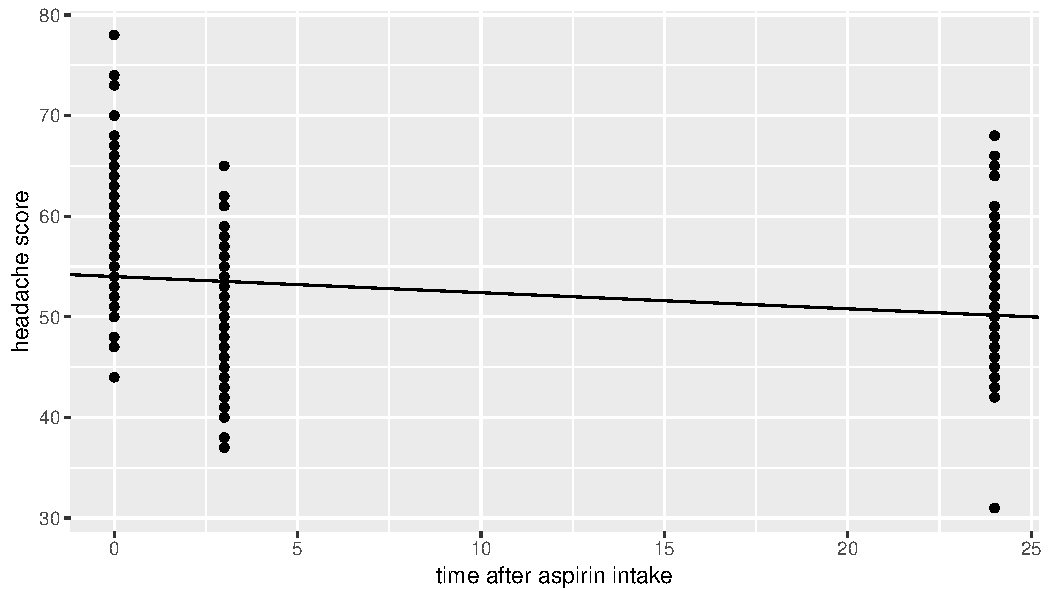
\includegraphics[width=\maxwidth]{figure/analysispremidpost5-1} 

}



\end{knitrout}

The line shown is the fitted line based on the SPSS output. It can be seen that the prediction for time=0 is too low, for time=2 too high, and for time=24 again too low. So for this particular data set on headache, it would be better to use a qualitative predictor for the effect of time on headache, like we did in the previous section.
\\
\\
As an example of a data set where a linear effect would have been appropriate, imagine that we measured headache 2 hours and 3 hours after aspirin intake (but not after 24 hours). Suppose these data would look like this:


\begin{knitrout}
\definecolor{shadecolor}{rgb}{0.969, 0.969, 0.969}\color{fgcolor}

{\centering 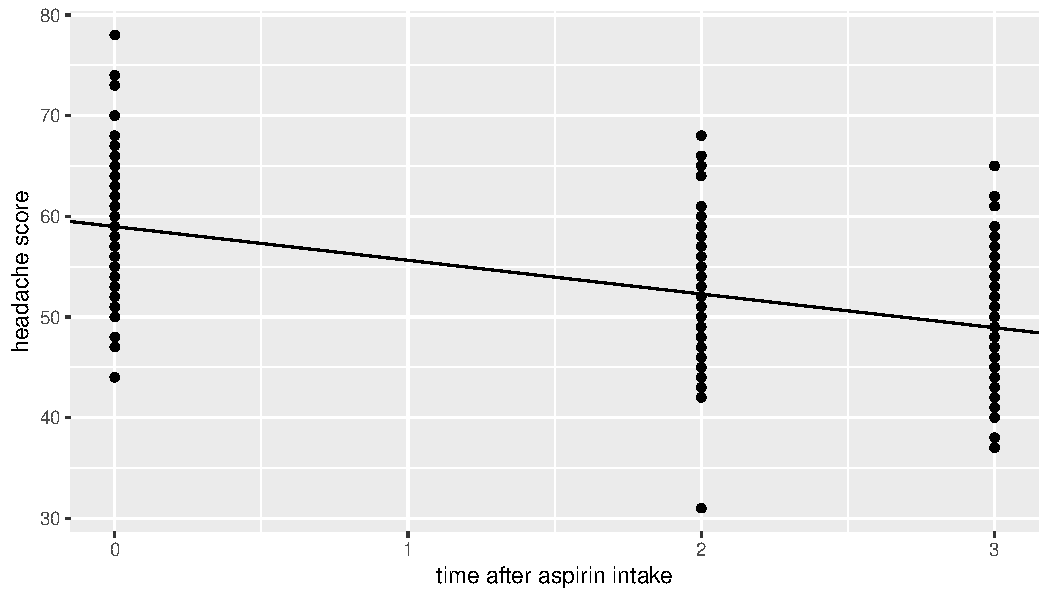
\includegraphics[width=\maxwidth]{figure/analysispremidpost6-1} 

}



\end{knitrout}

Here we see a gradual increase of headache levels right after aspirin intake. Here, a quantitative treatment of the time variable would be more appropriate. The SPSS output is given below.


\begin{figure}[h]
    \begin{center}
       \includegraphics[scale=0.8, trim={0cm 20cm 0cm 0cm} ]{/Users/stephanievandenberg/Dropbox/Statistiek_Onderwijs/Data" "Analysis/spss" "examples" "linear" "mixed" "model/premidpost/premidpostaspirinlinear2.pdf}
    \end{center}
\end{figure}


From the output we see that the intercept is 59 and that the slope is -3.3. So this model predicts an hourly decrease of 3.3 points in headache level. This regression line is also depicted in the above figure. 

Because we are confident that this model is appropriate for our data, we can interpret the statistical output from SPSS. 

\begin{quotation}
A linear mixed model was run, using a quantitive variable time and random effects for the variable patient. We saw a significant linear effect of time on headache level, $t(199)=-24.42, p < 0.001$. The estimated effect of time based on this analysis is negative, $-3.3$, so with every hour that elapses after aspirin intake, the predicted headache score decreases with 3.3 points. 
\end{quotation}


\subsection{Exercises}

Suppose you have a number of CEOs with smart watches and you have these smart watches log skin conductance. Skin conductance is a good measure for stress. These measurements are done at random intervals, for at most 4 times during one day. The experiment starts at 7am and stops at 7pm. The \textbf{time} variable measures how many hours have passed since 7am.
 \\
 \\
 \begin{tabular}{lrr}
 CEO & time & conductance \\ \hline
 001 & 2 & 80 \\
 001 & 3 & 65 \\
 001 & 10 & 60 \\
 001 & 11 & 60 \\
 002 & 4 & 34 \\
 002 & 6 & 25 \\
 002 & 9 & 30 \\
 002 & 12 & 30 \\
 003 & 3 & 23 \\
 003 & 4 & 15 \\
 003 & 5 & 20 \\
 003 & 8 & 20 \\
 004 & 0 & 90 \\
 004 & 3 & 70 \\
 004 & 4 & 65 \\
 004 & 11 & 65 \\
 \dots & \dots & \dots \\
 \end{tabular}
\\
\\
Now you'd like to know if skin conductance in CEOs shows a general decrease during the day. Your null-hypothesis is therefore that there is no linear effect of time on skin conductance. Now, you have multiple measures for each CEO (repeated measures), and there might be individual differences in the average skin conductance that you would like to take into account. Therefore you perform a MIXED analysis in SPSS. 

\begin{itemize}
\item 1. What would the SPSS syntax look like? \\
\item 2. If you got the following output, what would your predicted skin conductance be for a CEO at 15.00 hrs? \\
\begin{figure}[h]
    \begin{center}
       \includegraphics[scale=0.5]{/Users/stephanievandenberg/Dropbox/Statistiek_Onderwijs/Data" "Analysis/spss" "examples" "mixed" "linear" "model/pre-mid-post" "design/CEOexample.png}
    \end{center}
\end{figure}



\item 3. Look at the data plotted: do you think a linear effect is reasonable for this data set?

\begin{knitrout}
\definecolor{shadecolor}{rgb}{0.969, 0.969, 0.969}\color{fgcolor}

{\centering 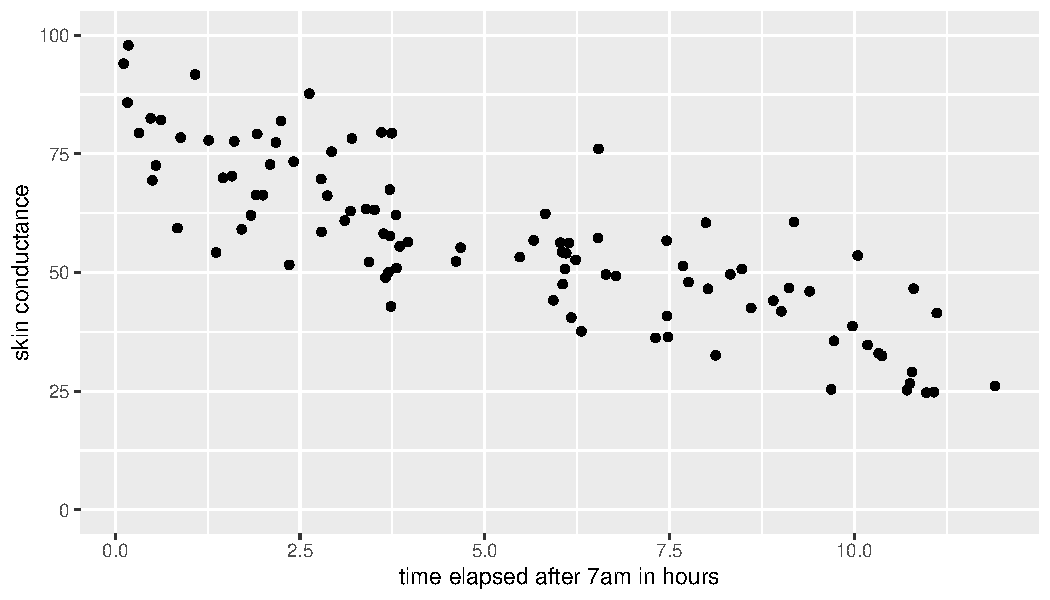
\includegraphics[width=\maxwidth]{figure/analysispremidpost7-1} 

}



\end{knitrout}




\item 4. How much clustering is there for skin conductance across CEOs? \\
\item 5. Would you say these individual differences are very important to take into account? \\
\item 6. Is there a significant effect of time of day on skin conductance in CEOs?\\
\item 7. What is the effect of time of day on skin conductance in CEOs? Also give the 95\% confidence interval of this effect.
\item 8. Write a short paragraph that describes the results in APA format.
\item 9. Given a new data set where every student's mood was tested at three points in time: During Christmas holidays (time points 1), during Easter holidays (time point 2) and at the start of the academic year, September 1 (time point 3). Look at the data plotted: do you think a linear effect is reasonable for this data set? Explain your answer.

\begin{knitrout}
\definecolor{shadecolor}{rgb}{0.969, 0.969, 0.969}\color{fgcolor}

{\centering 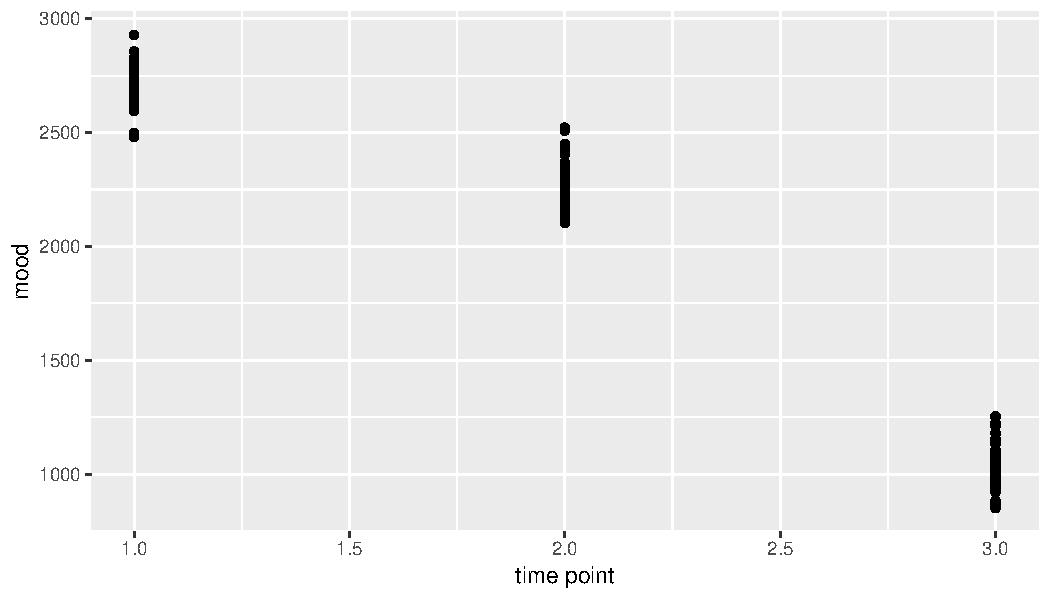
\includegraphics[width=\maxwidth]{figure/analysispremidpost8-1} 

}



\end{knitrout}

\item 10. Provide the syntax you would use to analyse the problem of question 9.


\end{itemize}

Answers:
\begin{itemize}
\item 1. \\
\begin{verbatim}
MIXED conductance WITH time
  /FIXED=time
  /PRINT=DESCRIPTIVES  SOLUTION
  /RANDOM=intercept | SUBJECT(CEO) COVTYPE(VC).
\end{verbatim}
\item 2. 15 hrs is equal to 8 hours after 7am, so the expected skin conductance is equal to $62 - 4 \times 8= 30$\\
\item 3. Yes, a general linear downward trend is observed for the skin conductance.
\item 4. The intraclass correlation coefficient is equal to $\frac{235}{235+247}=0.49$, 
\item 5. The correlation is quite different from 0, so there is certainly some clustering in the data and it is important to take these individual differences into account. \\
\item 6. Yes, there is a signficant linear effect of time on skin conductance in CEOs, $t(59)=-4.24, p < 0.01$.\\
\item 7. The linear effect of time of day on skin conductance in CEOs is around -4.13 points per hour after 7am (95 \% CI: -6.08 -- -2.18). \\
\item 8. \begin{quotation}
        A linear mixed model was run with time as a quantitative predictor for skin conductance, including random effects for CEO. We found an effect of time of -4.13 points per hour which was significantly different from 0, $t(59)=-4.24, p < 0.001$. Therefore we conclude that time of day has an effect on skin conductance in the entire population of CEOs.
        \end{quotation}
        
\item 9. The relationship is not linear: you cannot draw a straight line through the means of the three measurements. 
\item 10. Because we have multiple measurements from the same students we should use a MIXED analysis. Furthermore, a qualitave analysis would be more suitable, given the nonlinear relationship between time and mood. So we use the syntax:

\begin{verbatim}
MIXED mood BY time
  /FIXED=time
  /PRINT=DESCRIPTIVES  SOLUTION
  /RANDOM=intercept | SUBJECT(student) COVTYPE(VC).
\end{verbatim}

\end{itemize}



\section{Linear mixed models and interaction effects}


Suppose we carry out the aspirin and headache study not only with a random sample of NY Times readers that suffer from regular headaches, but also with a random sample of readers of the Wall Street Journal that suffer from regular headaches. We'd like to know whether aspirin works, but we are also interested to know whether the effect of aspirin is similar in the two groups of readers. Our null-hypothesis is that the effect of aspirin in affecting headache severity is the same in NY Times and Wall Street Journal readers that suffer from headache.\\
\\
H\_0: The effect of aspirin is the same for NY Times readers as for Wall Street Journal readers.
\\
\\
Suppose we have the following data set (we only show the first six patients), and we only look at the measurements before aspirin intake and 3 hours after aspirin intake (pre-post design):

\begin{knitrout}
\definecolor{shadecolor}{rgb}{0.969, 0.969, 0.969}\color{fgcolor}
\begin{tabular}{r|l|r|r}
\hline
patient & group & pre & post\\
\hline
1 & NYTimes & 55 & 45\\
\hline
2 & WallStreetJ & 63 & 50\\
\hline
3 & NYTimes & 66 & 56\\
\hline
4 & WallStreetJ & 50 & 37\\
\hline
5 & NYTimes & 63 & 50\\
\hline
6 & WallStreetJ & 65 & 53\\
\hline
\end{tabular}


\end{knitrout}



In this part of the data set, patients 2, 4, and 6 read the Wall Street Journal, and patients 1, 3 and 5 read the NY Times. We assume that people only read one of these newspapers. We measure their headache before and after the intake of aspirin (a pre-post design). The data are now in what we call \textit{wide format}: the dependent variable \textbf{headache} is spread over two columns, \textbf{pre} and \textbf{post}. In order to analyse the data with linear models, we need them in \textit{long format}, like this:

\begin{knitrout}
\definecolor{shadecolor}{rgb}{0.969, 0.969, 0.969}\color{fgcolor}
\begin{tabular}{r|l|r|r}
\hline
patient & group & measure & headache\\
\hline
1 & NYTimes & 1 & 55\\
\hline
1 & NYTimes & 2 & 45\\
\hline
2 & WallStreetJ & 1 & 63\\
\hline
2 & WallStreetJ & 2 & 50\\
\hline
3 & NYTimes & 1 & 66\\
\hline
3 & NYTimes & 2 & 56\\
\hline
\end{tabular}


\end{knitrout}


The new variable \textbf{measure} now indicates whether a given measurement of headache refers to a measurement before intake (first measurement) or after intake (second measurement). Again we could investigate whether there is an effect of aspirin with a linear mixed model, with \textbf{measure} as our qualitative predictor, but that is not really what we want to test: we only want to know whether the effect of aspirin (being small, large, negative or non-existent) \textit{is the same for both groups}. Remember that this hypothesis states that there is no interaction effect of aspirin (\textbf{measure}) and group. The null-hypothesis is that group is \textit{not} a moderator of the effect of aspirin on headache. There may be an effect of aspirin or there may not, and there may be an effect of newspaper (\textbf{group}) or there may not, but we're interested in the \textit{interaction} of aspirin and group membership. Is the effect of aspirin different for NY times readers than for Wall Street Journal readers?

In our analysis we therefore need to specify an interaction effect. Since the data are clustered (2 measures per patient), we use a linear \textit{mixed} model. First we show how to analyse these data using dummy variables, later we will show the results using a different approach. 
\\
\\
We recode the data into two dummy variables, one for the aspirin intervention (measure), and one for group membership. 

\begin{verbatim}
RECODE measure (1=0) (2=1) INTO post.
RECODE group ('WallStreetJ'=0) ('NYTimes'=1) INTO NYTimes.
EXECUTE.
\end{verbatim}

Next we need to compute the product of these two dummies to code for the interaction effect. Since with the above dummy coding, all post measures get a 1, and all NYTimes readers get a 1, only the observations that are post aspirin and that are from NYTimes readers get a 1 for the product, the interactiondummy . That's why it is best to name this interaction effect PostNYTimes. 

\begin{verbatim}
COMPUTE PostNYTimes=post*NYTimes.
EXECUTE.
\end{verbatim}

With these three new dummy variables we can specify the linear mixed model.

\begin{verbatim}
MIXED headache WITH post NYTimes PostNYTimes
  /FIXED= post NYTimes PostNYTimes
  /PRINT=DESCRIPTIVES  SOLUTION
  /RANDOM=intercept | SUBJECT(patient) COVTYPE(VC).
\end{verbatim}


In the output below, we recognize the three fixed effects for the three dummy variables. Since we're interested in the interaction effect, we look at the effect of PostNYTimes. The effect is in the order of +0.6. So what does this mean? 

\begin{figure}[h]
    \begin{center}
       \includegraphics[scale=0.8, trim={0cm 19cm 0cm 0cm}]{/Users/stephanievandenberg/Dropbox/Statistiek_Onderwijs/Data" "Analysis/spss" "examples" "linear" "mixed" "model/mixedprepost/mixedprepostdummy.pdf}
    \end{center}
\end{figure}



Remember that a reader from the Wall Street Journal gets a 0 for the group dummy \textbf{NYTimes}. All headache measures before aspirin intake are given a 0 for the intervention dummy \textbf{post}. 
Since the product of $ 0\times 0$ equals 0, all these measures before aspirin in Wallstreet Journal readers get a 0 for the interaction dummy \textbf{PostNYTimes}.
Therefore, the intercept of 59.5 refers to the expected headache severity of Wall Street Journal readers \textit{before} they take their aspirin. This is significantly different from zero, meaning that in the population of Wall Street Journal readers, headache before aspirin intake is different from zero.

Furthermore, we see that the effect of the intervention is -10.7. So, relative to Wall Street Journal readers prior to aspirin intake, the level of post intake headache is 10.7 points \textit{less}. So in the population of Wall Street Journal readers, the effect of aspirin is different from 0, since the effect of -10.7 is significant. 

If we look further down in the table, we see the effect of NYTimes equals 0.32. So, relative to Wall Street Journal readers, before aspirin intake (the reference group), NY Times readers score on average 0.32 points higher on the headache scale before aspirin intake. 

However, we're not interested in a general difference between those two groups of readers, we're interested in the effect of aspirin and whether it is different in the two groups of readers. In the last row we see the interaction effect: being a reader of the NY Times AND at the same time being a measure after aspirin intake, the expected increase in mean headache equals 0.60. So the effect of aspirin is -10.7 in Wall Street Journal readers, as we saw above, but the  effect is $-10.7 + 0.6 = -10.1$ in NY Times readers. So in this sample the effect of aspirin on headache is 0.6 \textit{smaller} than in Wall Street Journal readers (note that even while the interaction effect is positive, it is positive on a scale where a high score means more headache). 


Let's look at it in the different way, using a table with the dummy codes. For each group of data, pre or post aspirin and New York Times readers and Wall Street Journal readers, we note the dummy codes for the new dummy variables. In the last column we use the output estimates and multiply them with the respective dummy codes (1 and 0) to obtain the expected headache level (using rounded numbers):
\\
 \\
 \begin{tabular}{llrrrr}
  measure & group & post & NYTimes & PostNYT & exp mean \\ \hline
  pre   & WallStreet      &  0 & 0 & 0 & $60$ \\
 post   &  WallStreet     &  1 & 0 & 0 & $60 + (-11)=49$ \\
 pre    & NYtimes         &  0 & 1 & 0 & $60 + 0.3=60.3$  \\
 post   &  NYtimes        &  1 & 1 & 1 & $60 +(-11) + 0.3 + 0.6=49.9$ \\
 \end{tabular}
\\
\\
The exact numbers are displayed in the graph below:

\begin{knitrout}
\definecolor{shadecolor}{rgb}{0.969, 0.969, 0.969}\color{fgcolor}

{\centering 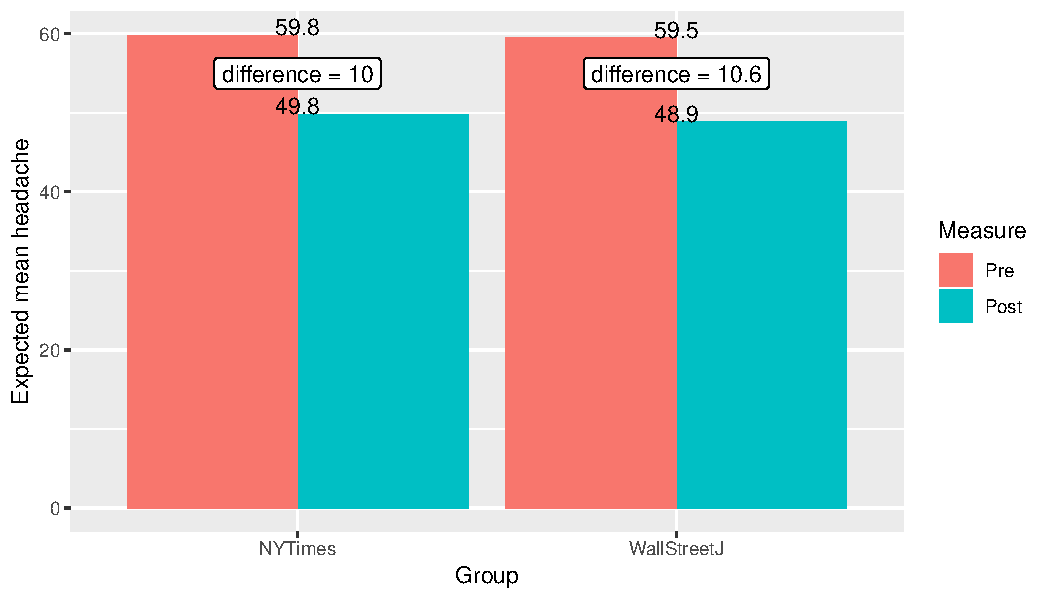
\includegraphics[width=\maxwidth]{figure/analysisprepostmixed3-1} 

}



\end{knitrout}


We see that the specific effect of aspirin in NYTimes readers is 0.6 smaller than the effect of aspirin in Wall Street Journal readers. This difference in the effect of aspirin between the groups was not significantly different from 0. The null-hypothesis that the effect is the same in the two populations of readers cannot be rejected. We therefore conclude that the effect that aspirin has on patients is the same for NY Times and Wall Street Journal readers. 

Note that we could have done the analysis in another way, not treating the variables in a quantitative way and using dummy variables, but by treating them qualitatively using the key word BY. The SPSS syntax would then be:

\begin{verbatim}
MIXED headache BY measure group 
  /FIXED=measure group measure*group
  /PRINT=DESCRIPTIVES  SOLUTION
  /RANDOM=intercept | SUBJECT(patient) COVTYPE(VC).
\end{verbatim}


The output would then look like below:


\begin{figure}[h]
    \begin{center}
       \includegraphics[scale=0.8, trim={0cm 15cm 0cm 0cm}]{/Users/stephanievandenberg/Dropbox/Statistiek_Onderwijs/Data" "Analysis/spss" "examples" "linear" "mixed" "model/mixedprepost/mixedprepostquali.pdf}
    \end{center}
\end{figure}



Here SPSS has automatically created dummy variables, one for \textbf{measure=1}, one for \textbf{group=1}, and one for the interaction effect, \textbf{group=1 AND measure=1}. Because the dummy coding is different, the intercept and the main effects of group and measure have changed, but you see that the interaction effect is still 0.6, albeit now negative. We also see that the significance level of the interaction effect is still the same. You are always free to choose to either construct your own dummy variables and analyze them in a quantitative way (using WITH), or to let SPSS construct the dummy variables for you (using BY): the $p$-value for the interaction effect will always be the same (this is not true for the intercept and the main effects).

Because the two analyses are equivalent (they end up with exactly the same predictions, feel free to check!), we can safely report that we've found a nonsignificant group by measure interaction effect, $t(98)=0.74, p=0.46$. We therefore conclude that in the populations of NY Times readers and Wall Street Journal readers, the short-term effect of aspirin on headache is the same. 



\subsection{Exercises}

Below we see data from a study on the effects of the financial crisis on the number of employees in specific Dutch companies. The companies are distinguised into food and non-food related companies. The number of employees are recorded in January 2008 and January 2011.

\begin{knitrout}
\definecolor{shadecolor}{rgb}{0.969, 0.969, 0.969}\color{fgcolor}
\begin{tabular}{r|l|r|r}
\hline
company & food & 2008 & 2011\\
\hline
1 & nonfood & 42 & 63\\
\hline
2 & food & 104 & 126\\
\hline
3 & nonfood & 76 & 58\\
\hline
4 & food & 65 & 131\\
\hline
\end{tabular}


\end{knitrout}

\begin{enumerate}
\item These data are in wide format. Rewrite the datamatrix in such a way that we have the same data in long format. Provide column (variable) names. 
\\
 \\
 \begin{tabular}{llrrrr}
   & \dots & \dots  & \dots & \dots  & \dots  \\ \hline
  & \dots & \dots  & \dots & \dots  & \dots  \\
  & \dots & \dots  & \dots & \dots  & \dots  \\
  & \dots & \dots  & \dots & \dots  & \dots  \\
  & \dots & \dots  & \dots & \dots  & \dots  \\
  & \dots & \dots  & \dots & \dots  & \dots  \\
  & \dots & \dots  & \dots & \dots  & \dots  \\
  & \dots & \dots  & \dots & \dots  & \dots  \\
  & \dots & \dots  & \dots & \dots  & \dots  \\
  & \dots & \dots  & \dots & \dots  & \dots  \\
  & \dots & \dots  & \dots & \dots  & \dots  \\
  & \dots & \dots  & \dots & \dots  & \dots  \\
  & \dots & \dots  & \dots & \dots  & \dots  \\
 \end{tabular}
\\
\\
\item Do we need to use a linear mixed model, or can we analyse these data with an ordinary linear model?
\item We want to test the null-hypothesis that the effects of the financial crisis in 2008 has the same effect on the number of employees in the food sector as in the non-food sector. Provide the syntax that helps you test this hypothesis. 
\item Suppose the following output results from an analysis done by a colleague:

\begin{figure}[h]
    \begin{center}
       \includegraphics[scale=0.8, trim={0cm 15cm 0cm 0cm}]{/Users/stephanievandenberg/Dropbox/Statistiek_Onderwijs/Data" "Analysis/spss" "examples" "linear" "mixed" "model/mixedprepost/mixedprepostemployee.pdf}
    \end{center}
\end{figure}

She provides you with the information that food=1 means the food sector and food=2 is the nonfood sector.

What does the model predict regarding the number of employees in 2008 in the non-food sector?
\item What does the model predict regarding the number of employees in 2011 in the non-food sector?
\item What does the model predict regarding the number of employees in 2008 in the food sector?
\item What does the model predict regarding the number of employees in 2011 in the food sector?
\item How large is the effect of the crisis in the food sector?
\item How large is the effect of the crisis in the non-food sector
\item How large is the intraclass correlation (ICC)? Give the computation.
\item Could we have done the analysis with an ordinary linear model? Explain your answer.
\item Can we reject the null-hypothesis that the effects of the crisis were the same in the food and non-food sectors? Explain your answer.
\end{enumerate}


Answers:
\\
\begin{enumerate}
\item It could look like this:
\\
\\
\begin{tabular}{llrrrr}
   & company & sector  & year & NEmployees  & \dots  \\ \hline
  & 1 & nonfood  & 2008 & 42  & \dots  \\
  & 1 & nonfood  & 2011 & 63  & \dots  \\
  & 2 & food  & 2008 & 104  & \dots  \\
  & 2 & food  & 2011 & 126  & \dots  \\
  & 3 & nonfood  & 2008 & 76  & \dots  \\
  & 3 & nonfood  & 2011 & 58  & \dots  \\
  & 4 & food  & 2008 & 65  & \dots  \\
  & 4 & food  & 2011 & 131  & \dots  \\
\end{tabular}
\\
\\
\item The data are clustered into companies: for each company we have two data points, so we should at least try a linear mixed model. Only if the variance of the company random effects is extremely small, we could use a linear model without random effects.
\item One option is to let SPSS construct the dummy variables:

\begin{verbatim}
MIXED employees BY year sector 
  /FIXED=year sector year*sector
  /PRINT=DESCRIPTIVES  SOLUTION
  /RANDOM=intercept | SUBJECT(company) COVTYPE(VC).
\end{verbatim}

Or you do the dummy coding yourself, for example like this:

\begin{verbatim}

RECODE year (2008=0) (2011=1) INTO year2011.
RECODE sector ('Nonfood'=0) ('food'=1) INTO food.
EXECUTE.

COMPUTE food2011=year2011*food.
EXECUTE.

MIXED employees WITH year2011 food food2011
  /FIXED= year2011 food food2011
  /PRINT=DESCRIPTIVES  SOLUTION
  /RANDOM=intercept | SUBJECT(company) COVTYPE(VC).
\end{verbatim}

\item the nonfood sector is food=2, so the predicted number of employees in 2008 in the nonfood sector is equal to $81.57 + 0 -22.056 + 0= 59.514$
\item the nonfood sector is food=2, so the predicted number of employees in 2011 in the nonfood sector is equal to $81.57 + 0 + 0 + 0= 81.57$
\item the food sector is food=1, so the predicted number of employees in 2008 in the food sector is equal to $81.57 + 39.31 -22.056 + 0.85=99.674 $
\item the food sector is food=1, so the predicted number of employees in 2011 in the food sector is equal to $81.57 + 39.31 + 0 + 0 = 120.88   $ 
\item in the food sector the effect is a $120.88 - 99.674 =   21.206$ increase in number of employees
\item in the non-food sector the effect is a $81.57 - 59.514 =   22.056$ increase in number of employees
\item the ICC is $\frac{12}{12+208}=0.05$
\item we have clustering, with multiple data point per company, so in general a linear mixed model is better than an ordinary linear model. However, since the intraclass correlation is rather low, the results would be very similar if we would use an ordinary linear model.
\item The null-hypothesis cannot be reject as the year by sector interaction effect is not signifcantly different from 0, $t(998)=0.66, p=0.51$. (alternatively, $F(1,998)=0.44, p=0.51$). Note however that the statistical results are in terms of absolute number of employees. These data show that the average number of employees in 2008 is larger in the food sector than in the non-food sector. Perhaps it would be wiser to look at percentage increase in number of employees: A change from 100 to 102 reflects a larger impact than a change from 1000 to 1002.

\end{enumerate}





\section{Mixed designs}
The design in the previous section where we had both a grouping variable and a pre-post or repeated measures design, is often called a \textit{mixed design}. It is a mixed design in the sense that there are two kinds of variables: one is a \textit{between-individuals} variable, and one variable is a \textit{within-individual} variable. Here the between-individuals variable is \textbf{group}: two different populations of readers. It is called \textit{between} because one individual can only be part of one group. When we study the effect of the group effect we are essentially comparing the scores of one group of individuals with the scores of another group of individuals, so the comparison is \textit{between different individuals}. 
The two groups of data are said to be \textit{independent}, as we knew that none of the readers in this data set reads both journals. 

The within-variable in this design is the aspirin intervention, indicated by the variable \textbf{measure}. For each individual we have two observations: all individuals are present in both the pre condition data as well as in the post condition data. With this intervention variable, we are comparing the scores of a group of indiviudals with the scores \textit{of that same group of individuals} at another time point. The comparison of scores is within a particular individual, at timepoint 1 and at timepoint 2. So the pre and post sets of data are not independent: the headache scores in both conditions are coming from the same individuals. 

Mixed designs are often seen in psychological experiments. For instance, you want to know how large the effect of alcohol intake is on driving performance. You want to know whether the effect of alcohol on driving performance is the same in a Fiat 600 as in a Porsche. Suppose you have 100 participants for your study. There are many choices you can make regarding the design of your study. Here we discuss 4 alternative research designs:

\begin{enumerate}


\item One option is to have all participants participate in all four conditions: they all drive a Fiat with and without alcohol, and they all drive a Porsche, with and without alcohol. In this case, both the car and the alcohol are within-participant variables.

\item The second option is to have 50 participants drive a Porsche, with and without alcohol, and to have the other 50 participants drive the Fiat, with and without alcohol. In this case, the car is the between-participants variable, and alcohol is the within-participant variable. 

\item The third option is to have 50 participants without alcohol drive both the Porsche and the Fiat, and to have the other 50 participants drive the Porsche and the Fiat with alcohol. Now the car is the within-participant variable, and the alcohol is the between-participants variable.

\item The fourth option is to have 25 participants drive the Porsche with alcohol, 25 other participants drive the Porsche without alcohol, 25 participants drive the Fiat with alcohol, and the remaining 25 participants drive the Fiat without alcohol. Now both the car variable and the alcohol variable are between-participant variables: none of the participants is present in more than 1 condition.

\end{enumerate}

Only the second and the third design described here are mixed designs, having at least one between-participants variable and at least one within-participant variable. 

Remember that when there is at least one within variable in your design, you have to use a linear mixed model. If all variables are between variables, one can use an ordinary linear model. Note that the term \textit{mixed} in linear mixed model refers to the effects in the model that can be both random and fixed. The term \textit{mixed} in mixed designs refers to the mix of two kinds of variables: within variables and between variables. 

Also note that the within and between distinction refers to the units of analysis. If the unit of analysis is school, then the location of the school building is a between-school variable. An example of a within-school variable could be time: before a major curriculum reform and after a major curriculum reform. 

\subsection{Exercises}

\begin{enumerate}
\item A psychologist studies whether age affects math performance. In 2017, she measures math performance (one score) in a group of 80-year-olds and she measures math performance (one score) in a group of 90-year-olds. \\
1. In this design, is the age variable a between-participants variable or a within-participant variable?  \\
2. Would you analyze these data with a linear model, or with a linear mixed model? Explain. 
\\
\\
\item A psychologist studies whether age affects math performance. She measures math performance (one score) in a group of 7-year-olds and she measures math performance again when the same children are 8 years old. \\
1. In this design, is the age variable a between-participants variable or a within-participant variable?  \\
2. Would you analyze these data with a linear model, or with a linear mixed model? Explain. 
\\
\\
\item Look at the data table below.
\\
 \\
 \begin{tabular}{rllr}
  ID & Nationality & Sex & Mathscore  \\ \hline
  1   & Dutch      &  Male & 67   \\
 2   &  Dutch     &  Female & 88   \\
 3    & German         &  Male & 50   \\
 4   &  German        &  Female & 98  \\
  \dots   & \dots        &  \dots& \dots  \\
 \end{tabular}
\\
\\
In this data set on Math performance, we see two variables, nationality and sex. What kind of variables are these: within-participant variables or between-participants variables? Explain.
\\
1. Would you call this a mixed design? Explain.\\
2. Would you analyze this data set with a linear model or with a linear mixed model? Explain.
\\
\\
\item Look at the data table below.
\\
 \\
 \begin{tabular}{rllr}
  ID & Nationality & Age & Mathscore  \\ \hline
  1   & Dutch      &  3 & 67   \\
 1   &  Dutch     &  5 & 88   \\
 2    & German         &  4 & 50   \\
 2   &  German        &  6 & 98  \\
  \dots   & \dots        &  \dots& \dots  \\
 \end{tabular}
\\
\\
In this data set on Math performance, we see two variables, nationality and age. What kind of variables are these: within-participant variables or between-participants variables? Explain.\\
1. Would you call this a mixed design? Explain.\\
2. Would you analyze this data set with a linear model or with a linear mixed model? Explain.
\\
\\
\item Look at the data table below.
\\
 \\
 \begin{tabular}{rllr}
  ID & Subject & Sex & Mood  \\ \hline
  1   & Psychology      &  Male & 67   \\
 1   &  Psychology     &  Female & 88   \\
 2    & Sociology         &  Female & 50   \\
 2   &  Sociology        &  Male & 98  \\
  \dots   & \dots        &  \dots& \dots  \\
 \end{tabular}
\\
\\
In this data set on mood in transsexuals, we see two variables, the subject they have a Master's degree in, and sex. What kind of variables are these: within-participant variables or between-participants variables? Explain.\\
1. Would you call this a mixed design? Explain.\\
2. Would you analyze this data set with a linear model or with a linear mixed model? Explain.\\
\\
\item Look at the data table below.
\\
 \\
 \begin{tabular}{lrrr}
  SchoolID & Country & Year & Avarage Mathscore  \\ \hline
 1   & The Netherlands      &  2010 & 67   \\
 1   &  The Netherlands     &  2011 & 88   \\
 1    & The Netherlands         &  2012 & 50   \\
 1   &  The Netherlands        &  2013 & 98  \\
 2   & Germany      &  2010 & 67   \\
 2   &  Germany     &  2011 & 88   \\
 2    & Germany         &  2012 & 50   \\
 2   &  Germany        &  2013 & 98  \\
  \dots   & \dots        &  \dots & \dots  \\
 \end{tabular}
\\
\\
In this data set on average Math performance in schools, we see two variables, country of the school and year of data collection. What kind of variables are these: within-school variables or between-schools variables? Explain.\\
1. Would you call this a mixed design? Explain.\\
2. Would you analyze this data set with a linear model or with a linear mixed model? Explain.\\

\end{enumerate}


Answers:

\begin{enumerate}

\item 

1. The age variable is a between-participants variable: some of the participants are 80 years old and some are 90 years old: none are both at the same time. Age discriminates between two sets of participants, so it is a between-participants variable.
2. Two groups of participants were studied. Because we only have one measure for each participant, there is no clustering, and we use an ordinary linear model.


\item
1. The age variable is a within-participants variable: children are studied twice and scores can therefore be compared within an individual.
2. One group of participants was studied and for each participant we have two math scores. Because we have more than one measure for each participant, we have to use a linear mixed model to account for clustering.

\item 
Each participant is either Dutch or German. This is a between-participants variable. Each participant is either male or female, sex discriminates between separate groups of participants, so sex is a between-participants variable.
1. This is \textit{not} a mixed design as it does not have both within-participant and between-participants independent variables. 
2. Because we only have one measure for each participant, there is no clustering, and we use an ordinary linear model.


\item 
Each participant is either Dutch or German. This is a between-participants variable.
On measurement 1 participants have a different age than on measurement 2. This is a within-participant variable.
1. This is a mixed design as it has both a within-participant and a between-participants independent variable. 
2. For each participant we have two math scores, so we would have to use a linear mixed model to account for clustering.

\item
Each participant has only one Master’s degree. This is a between-participants variable. Between the two measurements, participants change their sex. This is a within-participant variable: we can compare people's mood when they are male and when they are female.
1. This is a mixed design as it has both a within-participant and a between-participants independent variable. 
2. For each participant we have two mood scores, so we would have to use a linear mixed model to account for clustering.


\item

Each school is based in only one country and has measurements across four years. Country is a between-schools variable and year is a within-school variable.
1. This is a mixed design as it has both a within-school and a between-schools independent variable. 
1. For each school we have four average math scores, so we would have to use a linear mixed model to account for clustering.



\end{enumerate}





\section{Mixed design with a linear effect}

In an earlier section we looked at a mixed design where the between variable was \textbf{newspaper} and the within variabe was \textbf{measure}: pre or post. It was a 2 by 2 design ($2 \times 2$) design: 2 measures and 2 newspapers, where we were interested in the interaction effect. We wanted to know whether newspaper moderated the effect of aspirin on headache. We used the within variable \textbf{measure} in a qualitative way by dummy coding it. 

In an earlier section in this chapter we saw that we can also model linear effects in linear mixed models, where we treated the time variable quantitatively: 0hrs, 3hrs after aspirin intake and 24 hrs after intake. Here we will give an example of a $3 \times 20$ mixed design: we have a qualitative group (between) variable with 3 levels and a quantitative time (within) variable with 20 levels. The example is about stress in athletes that are going to partake in the 2018 Winter Olympics. Stress can be revealed in morning cortisol levels. In the 20 days preceding the start of the Olympics, each athlete was measured every morning after waking and before breakfast by letting them chew on cotton. The cortisol level in the saliva was then measured in the lab. Our research question is whether cortisol levels rise in athletes that prepare for the Olympics.

Three groups were studied. One group consisted of 50 athletes who were selected to partake in the Olympics, one group consisted of 50 athletes that were very good but were not selected to partake (Control group I) and one group consisted of 50 non-athlete spectators that were going to watch the games (Control group II). The null-hypothesis was that the linear change in cortisol levels during those 20 days was the same for the three groups: the Olympeans, Control group I and Control group II. 

Below you see part of the data, the first 6 measurements on person 1 that belongs to the group of Olympeans.

\begin{knitrout}
\definecolor{shadecolor}{rgb}{0.969, 0.969, 0.969}\color{fgcolor}
\begin{tabular}{r|l|r|r}
\hline
person & group & measure & cortisol\\
\hline
1 & Olympean & 1 & 19.41570\\
\hline
1 & Olympean & 2 & 20.21298\\
\hline
1 & Olympean & 3 & 22.15560\\
\hline
1 & Olympean & 4 & 23.10641\\
\hline
1 & Olympean & 5 & 23.69396\\
\hline
1 & Olympean & 6 & 21.91889\\
\hline
\end{tabular}


\end{knitrout}

When we plot the data, and use different colours for the three different groups, we already notice that the Olympeans show generally higher cortisol levels, but particulary at the end of the 20-day period.



\begin{knitrout}
\definecolor{shadecolor}{rgb}{0.969, 0.969, 0.969}\color{fgcolor}

{\centering 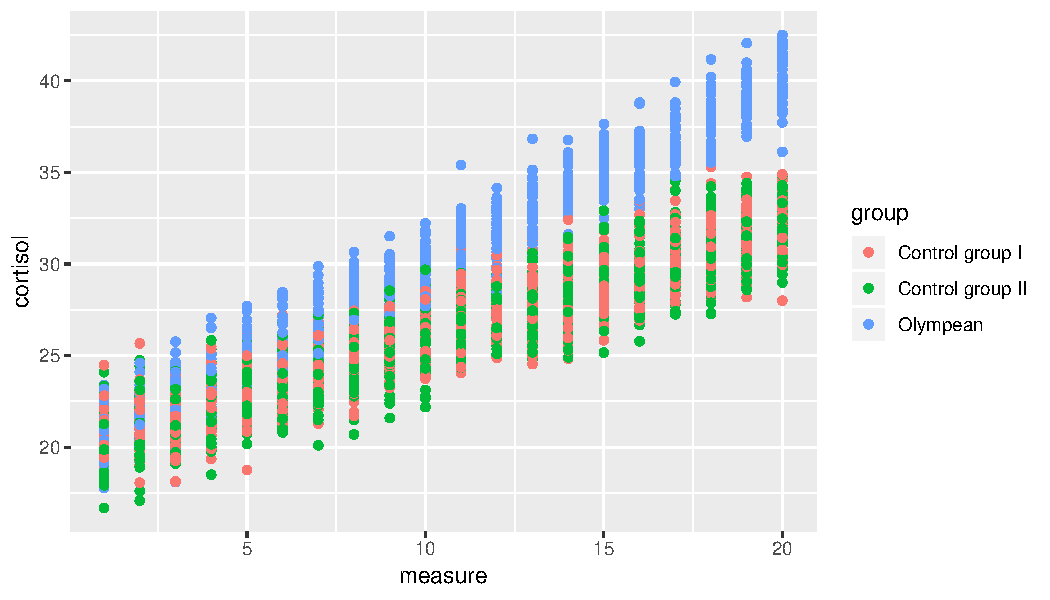
\includegraphics[width=\maxwidth]{figure/analysismixed20_2-1} 

}



\end{knitrout}

So we want to know whether the linear effect of time is moderated by group. Since for every person we have 20 measurements, the data are clustered so we use a linear mixed model. We're looking for a linear effect of time, so we use the WITH keyword to indicate that we want to use the \textbf{measure} variable in a quantitative way. We also use \textbf{group} as a predictor, but in a qualitative way, by using the keyword BY, so that SPSS will automatically make dummy variables. Because we're interested in an interaction effect, we include both main effects of \textbf{group} and \textbf{measure} and their interaction under the DESIGN subcommand. Lastly, we control for individual differences in cortisol levels by introducing a random effect for \textbf{person}.


\begin{verbatim}
MIXED cortisol WITH measure BY group 
  /FIXED=measure group measure*group
  /PRINT=DESCRIPTIVES  SOLUTION
  /RANDOM=intercept | SUBJECT(person) COVTYPE(VC).
\end{verbatim}


The SPSS output is presented below. 


\begin{figure}[h]
    \begin{center}
       \includegraphics[scale=0.8, trim={0cm 15cm 0cm 0cm}]{/Users/stephanievandenberg/Dropbox/Statistiek_Onderwijs/Data" "Analysis/spss" "examples" "linear" "mixed" "model/mixedprepost/mixed20.pdf}
    \end{center}
\end{figure}

In the output we see an intercept of 19.7, a slope of 1.0 for the effect of measure, two main effects for the group variable (group3 is the reference group, in this case the Olympeans, see the plot above), and two effects for the interaction effect (one for control group I and one for control group II). Let's fill in the linear equation based on this output:


\begin{eqnarray}
cortisol_{ij} = 19.7 + person_i + 1 \times measure + .4  ContrG1 + \nonumber\\
      0.18 ContrG2 -.4  ContrG1 \times measure -.4  ContrG2 \times measure+   e_{ij} \nonumber\\
person_i \sim N(0, \sigma_p^2 = 0.99)\nonumber\\
e_{ij} \sim N(0, \sigma_e^2 = 1.00) \nonumber
\end{eqnarray}

We see a clear intraclass correlation of around $\frac{0.986}{0.986+0.997}= 0.5 $ so it's a good thing we've included a random effect for persons. The expected means at various time points and for various groups can be made with the use of the above equation. 

It's easier to see what linear effects we have for the three different groups. Filling in the above equation for Control group 1, we get:

\begin{eqnarray}
cortisol_{ij} &=& 19.7 + person_i + 1 \times measure + .4    -.4  \times measure +   e_{ij} \nonumber \\
               &=&  20.1 + person_i +0.6 \times measure +   e_{ij} \nonumber
\end{eqnarray}

For Control group 2 we get:

\begin{eqnarray}
cortisol_{ij} &=& 19.7 + person_i + 1 \times measure  + 0.18  - .4  \times measure+   e_{ij} \nonumber \\
        &=&   19.88 + person_i   + 0.6 \times measure    +   e_{ij}    \nonumber
\end{eqnarray}

And for the Olympeans we get:

\begin{eqnarray}
cortisol_{ij} = 19.7 + person_i + 1 \times measure  +   e_{ij} \nonumber \\
\end{eqnarray}


In these equations all intercepts are around 20. The slopes are 0.6 in both Control groups I and II, whereas the slope is 1.0 in the group of Olympean athletes. For illustration, these implied linear regression lines are depicted below:


\begin{knitrout}
\definecolor{shadecolor}{rgb}{0.969, 0.969, 0.969}\color{fgcolor}

{\centering 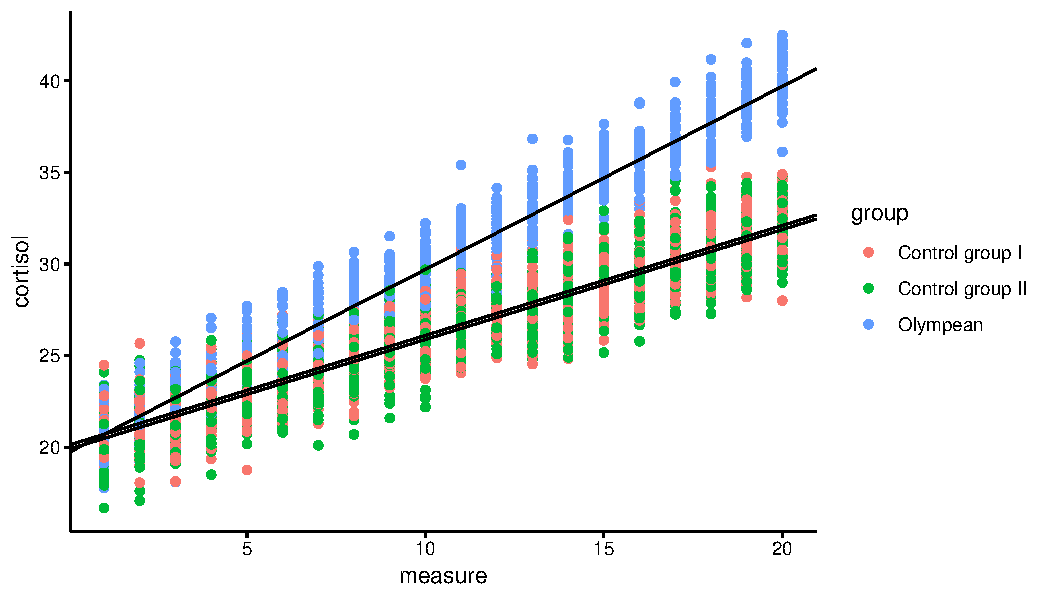
\includegraphics[width=\maxwidth]{figure/analysismixed20_3-1} 

}



\end{knitrout}

So based on the linear equation, we see that in this sample the rise in cortisol levels is much steeper in Olympeans than in the two control groups. But is this true for all Olympeans and the rest of the populations of high performing athletes and spectators? Note that in the regression table we see two interaction effects: one for \textbf{group1*measure} and one for \textbf{group2*measure}. Here we're interested in the overall signficance of the interaction effects. That answer we find in the top table with the $F$-statistics: we see a significant group by measure interaction effect, $F(2, 28)= 18.57, p<0.001$. The null-hypothesis of the same cortisol change in three different populations can be rejected, and we conclude that Olympean athletes, non-Olympean athletes and spectators show a different change in cortisol levels in the weeks preceding the games.  



 % introduction linear mixed models

\chapter{Non-parametric alternatives for linear mixed models}


\section{Checking assumptions}

In previous chapters we have discussed the assumptions of linear models and linear mixed models: linearity (in parameters), homoscedasticity (equal variance), normal distribution of residuals, normal distribution of random effects (relevant for linear mixed models only), and independence (no clustering unaccounted for). 




The problem of nonlinearity can be solved by introducing quadratic terms, for instance by replacing a linear model $Y = b_0 + b_1 X + e$ by another linear model $Y = b_0 + b_1 X + b_2 X^2 + e$.

If we have nonindependence, then you can introduce either an extra fixed effect or a random effect for this clustering. For example, if you see that cars owned by low income families have much more mileage than cars owned by high income families, you can account for this by adding a fixed effect of an income variable as predictor. If you see that average milage is rather similar within municipality but that average mileage can vary quite a lot across municipalities, you can introduce a random effect for municipality (if you have data say from 30 different municipalities). 

Unequal variance of residuals and nonnormal distribution of residuals are harder to tackle. Unequal variance can be tackled sometimes by using linear models, but with more advanced options, or by making corrections to $p$-values that make inference more robust against model violations. Violations of normality are even a bigger problem. Nonnormality can sometimes be solved by using generalized linear models (see next chapter). A combination of nonnormality and unequal variance can sometimes be solved by using a transformation of the data, for instance not analyzing $Y = b_0 + b_1 X + e$ but analyzing $log(Y)=  b_0 + b_1 X + e$ or $\sqrt{Y}=  b_0 + b_1 X + e$.

If these data transformations or advanced options don't work (or if you're not acquainted with them), and your data show nonequal variance and/or nonnormally distributed residuals, there are nonparametric alternatives.  Here we discuss two: Friedman's test and Wilcoxon's signed rank test. We explain them using an imaginary data set on speedskating.
\\
\\
Suppose we have data on 12 speedskaters that participate on the 10 kilometers distance in three separate championships in 2017-2018: the European Championships, the Winter Olympics and the World Championships. Your friend expects that speedskaters will perform best at the Olympic games, so there she expects the fastest times. So you decide to test the null-hypothesis that average times are the same at the three occasions. In Figure \ref{fig:nonparmixed_1} we see a boxplot of the data.

% H_0: $\mu_{EC}=\mu_{WC}_\mu{WO}$


\begin{knitrout}
\definecolor{shadecolor}{rgb}{0.969, 0.969, 0.969}\color{fgcolor}\begin{figure}

{\centering 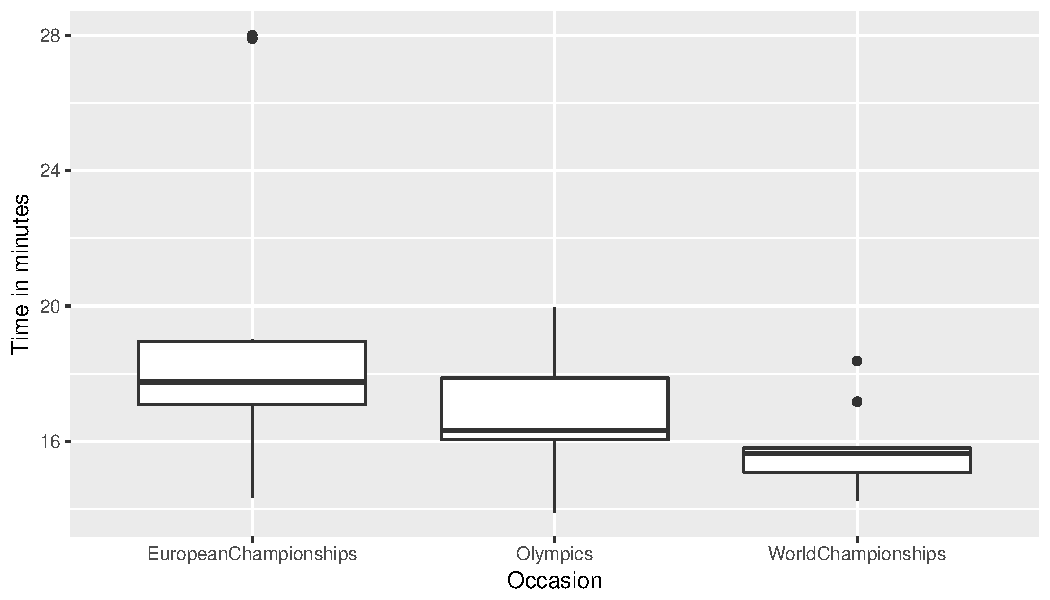
\includegraphics[width=\maxwidth]{figure/nonparmixed_1-1} 

}

\caption[Boxplot of the imaginary speed skating data]{Boxplot of the imaginary speed skating data.}\label{fig:nonparmixed_1}
\end{figure}


\end{knitrout}

In order to test this null-hypothesis, we run a linear mixed model with dependent variable time, and independent variable occasion. We use random effects for the differences in speed across skaters. In Figure \ref{fig:nonparmixed_2} we see the residuals:

\begin{knitrout}
\definecolor{shadecolor}{rgb}{0.969, 0.969, 0.969}\color{fgcolor}\begin{figure}

{\centering 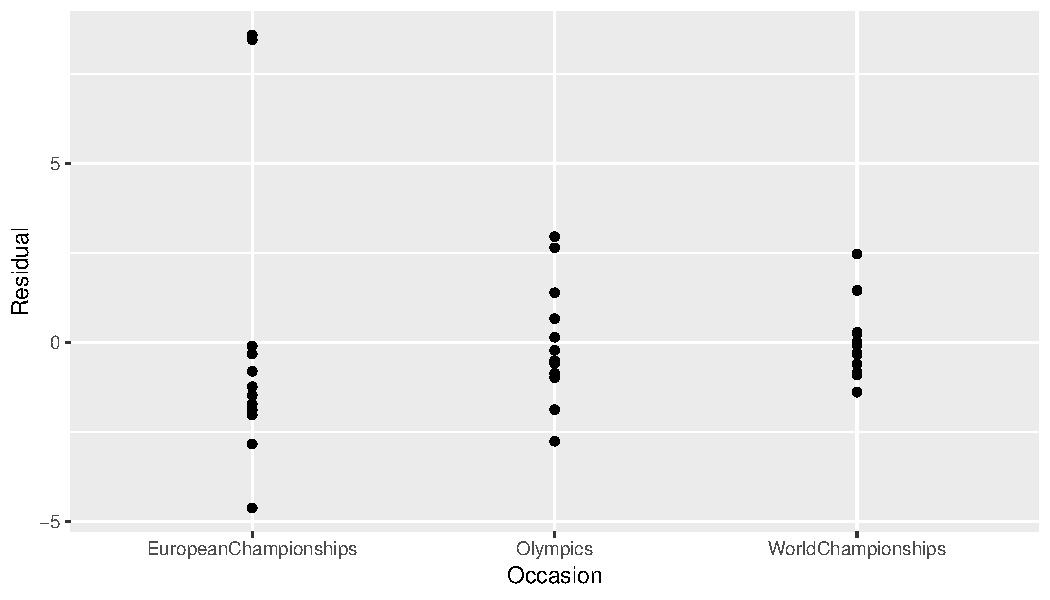
\includegraphics[width=\maxwidth]{figure/nonparmixed_2-1} 

}

\caption[Residuals of the speedskating data with a linear mixed model]{Residuals of the speedskating data with a linear mixed model.}\label{fig:nonparmixed_2}
\end{figure}


\end{knitrout}

From this plot we clearly see that the assumption of equal variance (homogeneity of variance) is violated: the variance of the residuals in the Worldchampionships condition is clearly smaller than the variance of the European championships condition. From the histogram of the residuals in Figure \ref{fig:nonparmixed_3} we also see that the distribution of the residuals is not bell-shaped: it is positively skewed (skewed to the right).




\begin{knitrout}
\definecolor{shadecolor}{rgb}{0.969, 0.969, 0.969}\color{fgcolor}\begin{figure}

{\centering 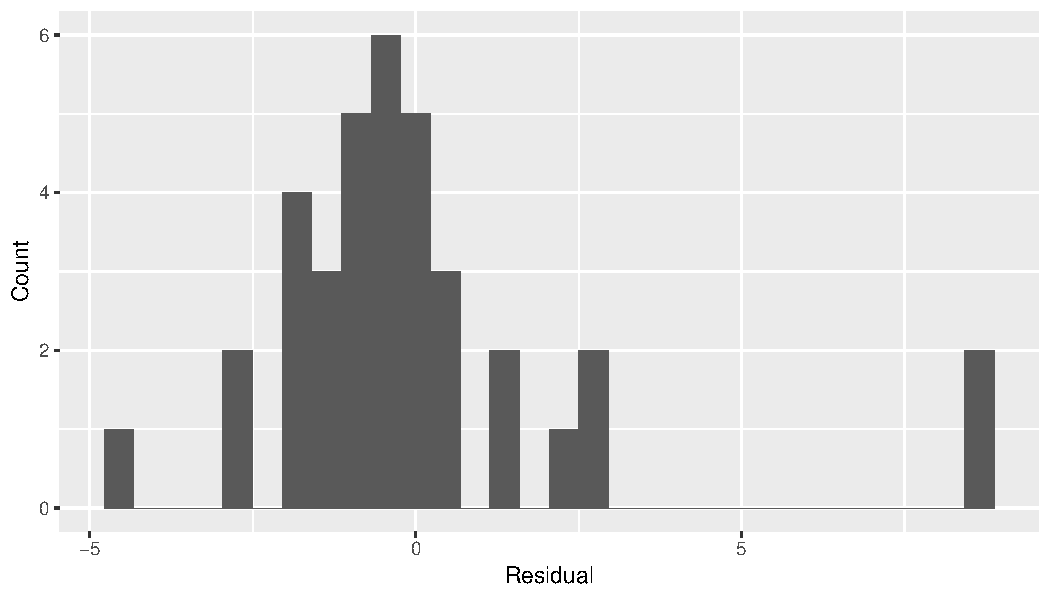
\includegraphics[width=\maxwidth]{figure/nonparmixed_3-1} 

}

\caption[Histogram of the residuals of the speedskating data with a linear mixed model]{Histogram of the residuals of the speedskating data with a linear mixed model.}\label{fig:nonparmixed_3}
\end{figure}


\end{knitrout}
% \\
% \\
Since the assumptions of homogeneity of variance and of normally distributed residuals are violated\footnote{Remember that assumptions relate to the population not samples: oftentimes your data set is too small to say anything about assumptions at the populationlevel. Residuals for a data set of 8 persons might show very nonnormal residuals, or very different variances for two subgroups of 4 persons each, but that might just be a coincidence, a random result because of the small sample size. If in doubt, it is best to use nonparametric methods.}, the results from the linear mixed model cannot be trusted. In order to answer our research question, we therefore have to resort to another kind of test. Here we discuss Friedman's test, a non-parametric test, for testing the null-hypothesis that the \textit{medians} of the three groups of data are the same. This Friedman test can be used in all situations where you have at least 2 levels of the within variable. In other words, you can use this test when you have data from three occasions, but also when you have data from 10 occassions or only 2. In the following section the Wilcoxon signed ranks test is discussed. This test is often used in social and behavioural sciences. The downside of this test is that it can only handle data sets with 2 levels of the within variable. In other words, it can only be used when we have data from two occassions. Friedman's test is therefore more generally applicable than Wilcoxon's. We therefore advise to always go with the Friedman test, but for the sake of completeness, we will also explain the Wilcoxon test.





\section{Friedman's test for $k$ measures}


Similar to many other nonparametric tests for testing the equality of medians, Friedman's test is based on ranks. Figure \ref{fig:nonparmixed_4} shows the speedskating data in wide format.


% latex table generated in R 3.4.2 by xtable 1.8-2 package
% Fri May  4 10:41:06 2018
\begin{table}[ht]
\centering
\caption{The speedskating data in wide format.} 
\label{tab:nonparmixed_4}
\begin{tabular}{lrrr}
  \hline
athlete & EuropeanChampionships & Olympics & WorldChampionships \\ 
  \hline
1 & 14.35 & 16.42 & 15.79 \\ 
  2 & 17.36 & 18.13 & 14.26 \\ 
  3 & 19.01 & 19.95 & 18.37 \\ 
  4 & 27.90 & 17.78 & 15.12 \\ 
  5 & 17.67 & 16.96 & 17.17 \\ 
  6 & 17.83 & 16.15 & 15.30 \\ 
  7 & 16.30 & 19.44 & 15.63 \\ 
  8 & 28.00 & 16.23 & 15.69 \\ 
  9 & 18.27 & 15.76 & 15.65 \\ 
  10 & 17.00 & 16.18 & 14.99 \\ 
  11 & 17.10 & 13.89 & 15.83 \\ 
  12 & 18.94 & 14.83 & 14.77 \\ 
   \hline
\end{tabular}
\end{table}


We rank all of these time measures by determining the fastest time, then the next to fastest time, etcetera, until the slowest time. But because the data in each row belong together (we compare individuals with themselves), we do the ranking \textit{row-wise}. For each athlete separately, we determine the fastest time (1), the next fastest time (2), and the slowest time (3) and put the ranks in a table.


% latex table generated in R 3.4.2 by xtable 1.8-2 package
% Fri May  4 10:41:06 2018
\begin{table}[ht]
\centering
\caption{Row-wise ranks of the speedskating data.} 
\label{tab:nonparmixed_5}
\begin{tabular}{lrrr}
  \hline
athlete & EuropeanChampionships & Olympics & WorldChampionships \\ 
  \hline
1 & 1.00 & 3.00 & 2.00 \\ 
  2 & 2.00 & 3.00 & 1.00 \\ 
  3 & 2.00 & 3.00 & 1.00 \\ 
  4 & 3.00 & 2.00 & 1.00 \\ 
  5 & 3.00 & 1.00 & 2.00 \\ 
  6 & 3.00 & 2.00 & 1.00 \\ 
  7 & 2.00 & 3.00 & 1.00 \\ 
  8 & 3.00 & 2.00 & 1.00 \\ 
  9 & 3.00 & 2.00 & 1.00 \\ 
  10 & 3.00 & 2.00 & 1.00 \\ 
  11 & 3.00 & 1.00 & 2.00 \\ 
  12 & 3.00 & 2.00 & 1.00 \\ 
   \hline
\end{tabular}
\end{table}


From this table we see for example that athlete 1 had the fastest time on the European Championships (14.35, rank 1) and the slowest at the Olympics (16.42, rank 3).


Next we compute the sum of the ranks column-wise: the sum of the ranks for the European Championships data is 31, for the Olympic data it's 26 and for the World Championships data it is 15.

From these sums we can gather that in general, these athletes showed their best times (many rank 1s) at the World Championships, as the sum of the ranks is lowest. We also see that in general these athletes showed their worst times (many rank 2s and 3s) at the European Championships, as the relevant column showed the highest sum of ranks.

In order to know whether these sums of ranks are significantly different from eachother, we may compute an $F_r$-value based on the following formula:


\begin{equation}
F_r = \left[  \frac{12}{Nk(k+1)} \Sigma^k_{j=1} S_j^2      \right] - 3N (k+1)
\end{equation}


In this formula, $N$ stands for the number of rows (12 athletes), $k$ stands for the number of columns (3 occasions), and $S_j^2$ stands for the squared sum of column $j$ ($31^2$, $26^2$ and $15^2$). If we fill in these numbers, we get:

\begin{eqnarray}
F_r &=& \left[  \frac{12}{12 \times  3(3+1)} \times (31^2 + 26^2 + 15^2)      \right] - 3 \times 12 (3+1) \nonumber \\
  &=&   \left[  \frac{12}{144} \times  1862      \right] - 144 = 11.17  \nonumber
\end{eqnarray}



What can we tell from this $F_r$-statistic? In order to say something about significance, we have to know what values are to be expected under the null-hypothesis that there are no differences across the three groups of data. Suppose we randomly mixed up the data by taking all the speedskating times and randomly assigning them to the three contests and the twelve athletes, until we have a newly filled datamatrix in Table \ref{tab:nonparmixed_26}:

% latex table generated in R 3.4.2 by xtable 1.8-2 package
% Fri May  4 10:41:06 2018
\begin{table}[ht]
\centering
\caption{The raw skating data in random order.} 
\label{tab:nonparmixed_26}
\begin{tabular}{lrrr}
  \hline
athlete & EuropeanChampionships & Olympics & WorldChampionships \\ 
  \hline
1 & 18.37 & 15.79 & 17.83 \\ 
  2 & 15.12 & 14.83 & 17.67 \\ 
  3 & 14.35 & 14.99 & 15.63 \\ 
  4 & 14.26 & 17.00 & 17.36 \\ 
  5 & 19.01 & 16.30 & 17.17 \\ 
  6 & 16.23 & 15.30 & 14.77 \\ 
  7 & 15.83 & 15.69 & 27.90 \\ 
  8 & 15.76 & 19.44 & 13.89 \\ 
  9 & 15.65 & 18.27 & 16.18 \\ 
  10 & 28.00 & 17.78 & 16.15 \\ 
  11 & 19.95 & 16.42 & 17.10 \\ 
  12 & 18.13 & 16.96 & 18.94 \\ 
   \hline
\end{tabular}
\end{table}


If we then compute $F_r$ for these mixed up data, we get another value. If we do this say 1000 times, we get the following values for $F_r$, summarized in the  histogram in Figure \ref{fig:nonparmixed_36}.

%fig.cap='Histogram of 1000 possible values for F_r given that the null-hypothesis is true, for 12 speedskaters.'

\begin{knitrout}
\definecolor{shadecolor}{rgb}{0.969, 0.969, 0.969}\color{fgcolor}\begin{figure}

{\centering \includegraphics[width=\maxwidth]{figure/nonparmixed_36-1} 

}

\caption[Histogram of 1000 possible values for Fr given that the null-hypothesis is true, for 12 speedskaters]{Histogram of 1000 possible values for Fr given that the null-hypothesis is true, for 12 speedskaters.}\label{fig:nonparmixed_36}
\end{figure}


\end{knitrout}

So if the data is just randomly distributed over the three columns in the data matrix, we expect no systematic differences and so the null-hypothesis is true. So now we know what the distribution of $F_r$ looks like when the null-hypothesis is true. Remember that for the true data that we actually gathered, we found an $F_r$-value of 11.17. From the histogram, we see that only very few values of 11.17 or larger are observed when the null-hypothesis is true. If we look more closely, we find that only 0.4\% of the values are larger than 11.17, so we have a $p$-value of 0.004. The 95th percentile of these 1000 $F_r$-values is 5.1666667, meaning that of the 1000 values for $F_r$, 5\% are larger than 5.1666667. So if we use a signficance level of 5\%, our observed value of 11.17 is larger than the critical value for $F_r$, and we conclude that the null-hypothesis can be rejected.

Now this $p$-value of 0.004 and the critical value of 5.1666667 are based on our own computations. Actually there are better ways. One is to look up critical values of $F_r$ in tables, for instance in Kendall M.G. (1970) \textit{Rank correlation methods}. (fourth edition). The $p$-value corresponding to this $F_r$-value depends on $k$, the number of groups of data (here 3 columns) and $N$, the number of rows (12 individuals). If we look up that table, we find that for $k=3$ and $N=12$ the critical value of $F_r$ for a type I error rate of 0.05 equals 6.17. Our observed $F_r$-value of 11.17 is larger than that, therefore we can reject the null-hypothesis that the median skating times are the same at the three different championships. So we have to tell your friend that there are general differences in skating times at different contests, $F_r=11.17, p < 0.05$, but it is not the case that the fastest times were observed at the Olympics.

Another way is to make an approximation of the distribution of $F_r$. Note that the distribution in the histogram is very strangely shaped. The reason is that the data set is quite limited. Suppose we have not data on 12 speedskaters, but on 120. If we then randomly mix up data again and compute 1000 different values for $F_r$, we get the histogram in Figure \ref{fig:nonparmixed_46}.


\begin{knitrout}
\definecolor{shadecolor}{rgb}{0.969, 0.969, 0.969}\color{fgcolor}\begin{figure}

{\centering \includegraphics[width=\maxwidth]{figure/nonparmixed_46-1} 

}

\caption[Histogram of 1000 possible values for Fr given that the null-hypothesis is true, for 120 speedskaters]{Histogram of 1000 possible values for Fr given that the null-hypothesis is true, for 120 speedskaters.}\label{fig:nonparmixed_46}
\end{figure}


\end{knitrout}

The shape becomes more regular. It also starts to resemble another distribution, that of the $\chi^2$ (chi-square). It can be shown that the distribution of the $F_r$ for a large number of rows in the data matrix, and at least 6 columns, approaches the shape of the $\chi^2$-distribution with $k-1$ degrees of freedom. This is shown in Figure \ref{fig:nonparmixed_56}.

\begin{knitrout}
\definecolor{shadecolor}{rgb}{0.969, 0.969, 0.969}\color{fgcolor}\begin{figure}

{\centering \includegraphics[width=\maxwidth]{figure/nonparmixed_56-1} 

}

\caption[The distrbution of Fr under the null-hypothesis, overlain with a chi-square distribution with 2 degrees of freedom]{The distrbution of Fr under the null-hypothesis, overlain with a chi-square distribution with 2 degrees of freedom.}\label{fig:nonparmixed_56}
\end{figure}


\end{knitrout}

The line of the $\chi^2$-distribution with 2 degrees of freedom approaches the histogram quite well, but not perfectly. In general, for large $N$ and $k>5$, the approximation is good enough. In that way it gets easier to look up $p$-values for certain $F_r$-values, because the $\chi^2$-distribution is well-known\footnote{The $\chi^2$-distribution is based on the normal distribution: the $\chi^2$-distribution with $k$ degrees of freedom is the distribution of a sum of the squares of $k$ independent standard normal random variables.}, so we don't have to look up critical values for $F_r$ in old tables. For a significance level of 5\%, the critical value of a $\chi^2$ with 2 degrees of freedom is 5.991. This is close to the value in the table for $F_r$ in old books: 6.17. The part of the $\chi^2$-distribution with 2 degrees of freedom that is larger than the observed 11.17 is 0.0037537, so our approximate $p$-value for our null-hypothesis is 0.004.


\section{How to perform Friedman's test in SPSS}

First of all, you need data in wide format. If your data happens to be in long format, use the CASETOVARS procedure to get the data in wide format. CASETOVARS requires your data to be ordered, so use the SORT CASE BY procedure before CASETOVARS. Suppose your data is in long format, as in Table \ref{tab:nonparmixed_6}.

% latex table generated in R 3.4.2 by xtable 1.8-2 package
% Fri May  4 10:41:12 2018
\begin{table}[ht]
\centering
\caption{The raw skating data in long data format.} 
\label{tab:nonparmixed_6}
\begin{tabular}{lrr}
  \hline
athlete & occasion & time \\ 
  \hline
1 & 1.00 & 14.35 \\ 
  1 & 2.00 & 16.42 \\ 
  1 & 3.00 & 15.79 \\ 
  2 & 1.00 & 17.36 \\ 
  2 & 2.00 & 18.13 \\ 
  2 & 3.00 & 14.26 \\ 
   \hline
\end{tabular}
\end{table}



Then the following syntax turns the data into wide format:


\begin{verbatim}
SORT CASES BY athlete occasion.
CASESTOVARS
  /ID=athlete
  /INDEX=occasion
  /GROUPBY=VARIABLE
 /SEPARATOR = "_".
\end{verbatim}


This creates the wide format data matrix in Table \ref{tab:nonparmixed_7}:


% latex table generated in R 3.4.2 by xtable 1.8-2 package
% Fri May  4 10:41:12 2018
\begin{table}[ht]
\centering
\caption{The raw skating data in wide data format after CASETOVARS} 
\label{tab:nonparmixed_7}
\begin{tabular}{lrrr}
  \hline
athlete & time\_1.00 & time\_2.00 & time\_3.00 \\ 
  \hline
1 & 14.35 & 16.42 & 15.79 \\ 
  2 & 17.36 & 18.13 & 14.26 \\ 
  3 & 19.01 & 19.95 & 18.37 \\ 
  4 & 27.90 & 17.78 & 15.12 \\ 
  5 & 17.67 & 16.96 & 17.17 \\ 
  6 & 17.83 & 16.15 & 15.30 \\ 
  7 & 16.30 & 19.44 & 15.63 \\ 
  8 & 28.00 & 16.23 & 15.69 \\ 
  9 & 18.27 & 15.76 & 15.65 \\ 
  10 & 17.00 & 16.18 & 14.99 \\ 
  11 & 17.10 & 13.89 & 15.83 \\ 
  12 & 18.94 & 14.83 & 14.77 \\ 
   \hline
\end{tabular}
\end{table}


Note the variable names: they start with the dependent variable time and are then indexed by the number of the occasion, 1.00, 2.00 and 3.00, that relate to European Championships, Olympic Games and World Championships, respectively.

We can then specify that we want Friedman's test by using the NPAR TESTS procedure with the FRIEDMAN subcommand and indicating which variables we want to use:

\begin{verbatim}
NPAR TESTS
/FRIEDMAN=time_1.00 time_2.00 time_3.00.
\end{verbatim}

\begin{figure}[h]
    \begin{center}
       \includegraphics[scale=0.8, trim={0cm 22cm 0cm 0cm}]{/Users/stephanievandenberg/Dropbox/Statistiek_Onderwijs/Data" "Analysis/spss" "examples" "nonparmixed/friedman1.pdf}
    \end{center}
     \caption{SPSS output of the Friedman test.}
    \label{fig:friedman1}
\end{figure}


In the output in Figure \ref{fig:friedman1} you first see the mean ranks. Note that if you multiply these by 12 (the number of rows), you get the sum of the ranks per column that we also computed above. Next you see a chi-square statistic, degrees of freedom, and an asymptotic $p$-value (Asymp. Sig.). Why don't we see an $F_r$-statistic?

The reason is, as discussed in the previous section, that for large number of measurements (columns) and a large number of individuals (rows), the $F_r$ statistic tends to behave like a chi-square, $\chi^2$, with $k-1$ degrees of freedom. So what we are looking at in this output is really an $F_r$-value of 11.17 (exactly the same value as we computed by hand in the previous section). In order to approximate the $p$-value, this value of 11.17 is interpreted as a chi-square ($\chi^2$), which with 2 degrees of freedom has a $p$-value of 0.004.


This asymptotic (approximated) $p$-value is the correct $p$-value if you have a lot of rows (large $N$) and at least 6 variables ($k>5$). If you do not have that, as we have here, this asymptotic $p$-value is only what it is: an approximation. If you want to have the exact $p$-value, then do

\begin{verbatim}
NPAR TESTS
/FRIEDMAN=time_1.00 time_2.00 time_3.00
/METHOD=EXACT.
\end{verbatim}

and then use the $p$-value under $exact sign.$, in this case 0.002, see Figure \ref{fig:friedman2}.

\begin{figure}[h]
    \begin{center}
       \includegraphics[scale=0.8, trim={0cm 22cm 0cm 0cm}]{/Users/stephanievandenberg/Dropbox/Statistiek_Onderwijs/Data" "Analysis/spss" "examples" "nonparmixed/friedman2.pdf}
    \end{center}
    \caption{SPSS output of the Friedman test with the exact p-value.}
    \label{fig:friedman2}
\end{figure}


Thus, a Friedman's test of equal medians showed that speedskaters show significantly different median times on the 10 kilometer distance at the three types of contests, $F_r=11.17, p=0.002$.



\section{Wilcoxon's signed ranks test for 2 measures}

Friedman's test can be used for 2 measures, 3 measures or even 10 measures. As stated earlier, the well-known Wilcoxon's test can only be used for 2 measures. For completeness, we also discuss that test here.
\\
\\
For each athlete, we take the difference in skating times and call it $d$, see Table \ref{tab:nonparmixed_77}. Next we rank these $d$-values, irrespective of sign, and call these ranks $rank_d$. From the table \ref{nonparmixed_77} we see that athlete 12 shows the smallest difference in skating times ($d$= 0.06, rank = 1) and athlete 2 the largest difference.

% latex table generated in R 3.4.2 by xtable 1.8-2 package
% Fri May  4 10:41:12 2018
\begin{table}[ht]
\centering
\caption{The raw skating data and the computations for Wilcoxon signed ranks test} 
\label{tab:nonparmixed_77}
\begin{tabular}{lrrrrr}
  \hline
athlete & Olympics & WorldChampionships & d & rank\_d & ranksign \\ 
  \hline
1 & 16.42 & 15.79 & 0.63 & 5.00 & 5.00 \\ 
  2 & 18.13 & 14.26 & 3.87 & 12.00 & 12.00 \\ 
  3 & 19.95 & 18.37 & 1.58 & 8.00 & 8.00 \\ 
  4 & 17.78 & 15.12 & 2.66 & 10.00 & 10.00 \\ 
  5 & 16.96 & 17.17 & -0.21 & 3.00 & -3.00 \\ 
  6 & 16.15 & 15.30 & 0.85 & 6.00 & 6.00 \\ 
  7 & 19.44 & 15.63 & 3.81 & 11.00 & 11.00 \\ 
  8 & 16.23 & 15.69 & 0.54 & 4.00 & 4.00 \\ 
  9 & 15.76 & 15.65 & 0.11 & 2.00 & 2.00 \\ 
  10 & 16.18 & 14.99 & 1.19 & 7.00 & 7.00 \\ 
  11 & 13.89 & 15.83 & -1.94 & 9.00 & -9.00 \\ 
  12 & 14.83 & 14.77 & 0.06 & 1.00 & 1.00 \\ 
   \hline
\end{tabular}
\end{table}


Next we indicate for each rank whether it belongs to a positive or a negative difference $d$ and call that variable \textbf{ranksign}.

Under the null-hypothesis, we expect that some of the larger $d$-values are positive and some of them negative, in a fairly equal amount. If we sum the ranks having plus-signs and sum the ranks having minus-signs, we would expect that these two sums are about equal, but only if the null-hypothesis is true. If the sums are very different, then we should reject this null-hypothesis. In order to see if the difference in sums is too large, we compute them as follows:


\begin{eqnarray}
T^+ &=& 5+ 12 + 8 +10+6+11+4 +2 +7 +1 = 66 \nonumber \\
T^- &=& 3 + 9= 12 \nonumber
\end{eqnarray}



To know whether $T^+$ is significantly larger than $T^-$, the value of $T^+$ can be looked up in a table, for instance in Siegel \& Castellan (1988). There we see that for $T^+$, with 12 rows, the probability of obtaining a $T^+$ of at least 66 is 0.0171. For a two-sided test (if we would have switched the columns of the two championships, we would have gotten a $T^-$ of 66 and a $T^+$ of 12!), we have to double this probability. So we end up with a $p$-value of $2 \times 0.0171=0.0342$.


In the table we find no critical values for large sample size $N$, but fortunately, similar to the Friedman test, we use an approximation using the normal distribution. It can be shown that for large sample sizes, the statistic $T^+$ is approximately normally distributed with mean


\begin{equation}
\mu = \frac{N(N+1)}{4}
\end{equation}

and variance:

\begin{equation}
\sigma^2= \frac {N(N+1)(2N+1)  }  {24}
\end{equation}


If we therefore standardize the $T^+$ by subtracting the $\mu$ and then dividing by the square root of the variance $\sqrt(\sigma^2)=\sigma$, we get a $Z$-value with mean 0 and standard deviation 1. To do that, we use the following formula:

\begin{equation}
Z = \frac{T^+ - \mu}{\sigma} =  \frac  { T^+ - N(N+1)/4} {\sqrt{N(N+1)(2N+1)/24}}
\end{equation}


Here $T^+$ is 66 and $N$ equals 12, so if we fill in the formula we get $Z= 2.1180543$. From the standard normal distribution we know that 5\% of the observations lie above 1.96 and below -1.96. So a value for $Z$ larger than 1.96 or smaller than -1.96 is enough evidence to reject the null-hypothesis. Here our $Z$-statistic is larger than 1.96, therefore we reject the null-hypothesis that the median skating times are the same at the World Championships and the Olympics. The $p$-value associated with a $Z$-score of 2.1180543 is 0.034.





\section{How to perform Wilcoxon's signed ranks test in SPSS}

If you want to use the Wilcoxon test, then use the following syntax:

\begin{verbatim}
NPAR TESTS
/WILCOXON=time_2.00 time_3.00
/METHOD=EXACT.
\end{verbatim}


\begin{figure}[h]
    \begin{center}
       \includegraphics[scale=0.8, trim={0cm 18cm 0cm 0cm}]{/Users/stephanievandenberg/Dropbox/Statistiek_Onderwijs/Data" "Analysis/spss" "examples" "nonparmixed/wilcoxon1.pdf}
    \end{center}
    \caption{SPSS output of the Wilcoxon test.}
    \label{fig:wilcoxon1}
\end{figure}

In the output in Figure \ref{fig:wilcoxon1} we see a $Z$-statistic, an asymptotic $p$-value, and two exact $p$-values. The reason that we see a $Z$-statistic is that the Wilcoxon $T^+$ statistic approaches a normal distribution in case we have a large number of observations (many rows). If $N>15$, the approximation is good enough so that the statistic can be interpreted as a $z$-score (standardized score with a normal distribution). That means that a $z$-score of 1.96 or larger or -1.96 or smaller can be regarded as significant at the 5\% significance level. Since the standard normal distribution is only an approximation, and we have $N=12$, we have to look at the exact significance level, which is in this case 0.034. We see that the exact $p$-value is in this case equal to the approximate $p$-value. Note that we use a two-sided test, to allow for the fact that random sampling could lead to a higher median for the Olympic Games or a higher median for the World Championships. We just want to know whether the null-hypothesis that the two medians differ can be rejected (in whatever direction) or not.
\\
\\


Let's compare the output with the Friedman test, but then only use the relevant variables in your syntax:

\begin{verbatim}
NPAR TESTS
/FRIEDMAN=  time_2.00 time_3.00
/METHOD=EXACT.
\end{verbatim}


In the output in Figure \ref{fig:friedman3} we see that the null-hypothesis of equal medians at the World Championships and the Olympic Games can be rejected, with a $p$-value of 0.039.

\begin{figure}[h]
    \begin{center}
       \includegraphics[scale=0.8, trim={0cm 22cm 0cm 0cm}]{/Users/stephanievandenberg/Dropbox/Statistiek_Onderwijs/Data" "Analysis/spss" "examples" "nonparmixed/friedman3.pdf}
    \end{center}
    \caption{SPSS output of the Friedman test for two measures.}
    \label{fig:friedman3}
\end{figure}



Note that both the Friedman and Wilcoxon tests come up with very similar $p$-values. Their rationales are very similar: Friedman's test is based on ranks and Wilcoxon's test is based on positive and negative differences between measures 1 and 2, so in fact ranks 1 and 2 for each row in the data matrix. Both can therefore be used in the case you have two measures. We recommend to use the Friedman test, since that test can be used in all situations where you have 2 or more measures per row. Wilcoxon's test can only be used if you have 2 measures per row.
\\
\\
In sum, we can report in two ways on our hypothesis regarding similar skating times at the World Championships and at the Olympics:

\begin{enumerate}

\item

\begin{quotation}
A Friedman test showed a significant difference between the 10km skating times at the World Championships and at the Olympics, $F_r = 5.33, p=0.04$. Athletes more often show their fastest times at the World Championships than can be expected due to chance.
\end{quotation}

\item

\begin{quotation}
A Wilcoxon signed ranks test showed a significant difference between the 10km skating times at the World Championships and at the Olympics, $Z = -2.12, p=0.03$. Athletes more often show their fastest times at the World Championships than can be expected due to chance.
\end{quotation}

\end{enumerate}

How do we know that the fastest times were at the World Championships? If we look at raw data above, that does not seem that obvious. But this conlusion is based on the sum of ranks: we saw a sum of ranks of 26 for the Olympics and 15 for the World Championships. So the average rank is lower at the World Championships.


\section{Ties}

Many nonparametric tests are based on ranks. For example, if we have the data sequence {0.1, 0.4, 0.5, 0.2}, we give these values the ranks {1, 3, 4, 2}, respectively. But in may data cases, data sequences cannot be ranked unequivocally. Let's look at the sequence {0.1, 0.4, 0.4, 0.2}. Here we have 2 values that are exactly the same. We say then that we have \textit{ties}. If we have ties in our data like the 0.4 in this case, one very often used option is to arbitrarily choose one of the 0.4 values as smaller than the other, and then average the ranks. Thus, we rank the data into {1, 3, 4, 2} and then average the tied observations: {1, 3.5, 3.5, 2}. As another example, suppose we have the sequence {23, 54, 54, 54, 19}, we turn this into ranks {2, 3, 4, 5, 1} and take the average of the ranks of the tied observations of 54: {2, 4, 4, 4, 1}. These ranks corrected for ties can then be used to compute the test statistic, for instance Friedman's $F_r$ or Wilcoxon's $Z$. However, in many cases, because of these corrections, a slightly different formula is to be used. So the formulas become a little bit different. This is all done in SPSS automatically. If you want to know more, see Siegel and Castellan (1988).




\section{Exercises}


A researcher is interested in the relationship between mood and day of the week: are people generally moodier on Monday than on Wednesday or Friday?

Below we see the data on 4 people that rated their mood from 1 (very moody) to 10 (not moody at all) on three separate days in a week in February: Day 1 is Monday, day 2 is Wednesday and day 3 is Friday:

\begin{knitrout}
\definecolor{shadecolor}{rgb}{0.969, 0.969, 0.969}\color{fgcolor}
\begin{tabular}{r|r|r}
\hline
ID & Day & Mood\\
\hline
1 & 1 & 3\\
\hline
1 & 2 & 5\\
\hline
1 & 3 & 8\\
\hline
2 & 1 & 4\\
\hline
2 & 2 & 7\\
\hline
2 & 3 & 6\\
\hline
3 & 1 & 2\\
\hline
3 & 2 & 4\\
\hline
3 & 3 & 1\\
\hline
4 & 1 & 9\\
\hline
4 & 2 & 5\\
\hline
4 & 3 & 3\\
\hline
\end{tabular}


\end{knitrout}

\begin{enumerate}

\item Put the data into wide format, and think of appropriate variable names
\\
 \\
 \begin{tabular}{llrrrr}
   & \dots & \dots  & \dots & \dots  & \dots  \\ \hline
  & \dots & \dots  & \dots & \dots  & \dots  \\
  & \dots & \dots  & \dots & \dots  & \dots  \\
  & \dots & \dots  & \dots & \dots  & \dots  \\
  & \dots & \dots  & \dots & \dots  & \dots  \\
  & \dots & \dots  & \dots & \dots  & \dots  \\
  & \dots & \dots  & \dots & \dots  & \dots  \\
  & \dots & \dots  & \dots & \dots  & \dots  \\
  & \dots & \dots  & \dots & \dots  & \dots  \\
  & \dots & \dots  & \dots & \dots  & \dots  \\
  & \dots & \dots  & \dots & \dots  & \dots  \\
  & \dots & \dots  & \dots & \dots  & \dots  \\
  & \dots & \dots  & \dots & \dots  & \dots  \\
 \end{tabular}
\\
\\
\item Rank these data row-wise: for each row determine the lowest mood (1), the second lowest mood (2) and the highest mood score (3)
\\
 \\
 \begin{tabular}{llrrrr}
   & \dots & \dots  & \dots & \dots  & \dots  \\ \hline
  & \dots & \dots  & \dots & \dots  & \dots  \\
  & \dots & \dots  & \dots & \dots  & \dots  \\
  & \dots & \dots  & \dots & \dots  & \dots  \\
  & \dots & \dots  & \dots & \dots  & \dots  \\
  & \dots & \dots  & \dots & \dots  & \dots  \\
  & \dots & \dots  & \dots & \dots  & \dots  \\
  & \dots & \dots  & \dots & \dots  & \dots  \\
  & \dots & \dots  & \dots & \dots  & \dots  \\
  & \dots & \dots  & \dots & \dots  & \dots  \\
  & \dots & \dots  & \dots & \dots  & \dots  \\
  & \dots & \dots  & \dots & \dots  & \dots  \\
  & \dots & \dots  & \dots & \dots  & \dots  \\
 \end{tabular}
\\
\\
\item Determine the column sums: the sum of the ranks for Monday, Wednesday and Friday.
\item How many rows do you have ($N$) and how many columns of data do you have ($k$)?
\item Compute $F_r$.
\item Copy the data into SPSS and run a Friedman's test. Should you ask for an exact $p$-value? Provide the syntax.
\item Suppose you get the SPSS output in Figure \label{ref:friedmanmood1}. What would your conclusion be regarding the research question about the relationship between moodiness and the day of the week?

\begin{figure}[h]
    \begin{center}
       \includegraphics[scale=0.8, trim={0cm 20cm 0cm 0cm}]{/Users/stephanievandenberg/Dropbox/Statistiek_Onderwijs/Data" "Analysis/spss" "examples" "nonparmixed/friedmanmood1.pdf}
    \end{center}
    \caption{SPSS output of a Friedman test.}
    \label{fig:friedmanmood1}
\end{figure}

\item
In this data set, for which day did we observe the personal best mood? How many of the individuals showed their best mood on that day?


\item
A linear mixed model was run on this data set. When checking model assumptions, we saw the following graphs in Figures \ref{fig:nonparmixed_11a} and \ref{fig:nonparmixed_11b}.

\begin{knitrout}
\definecolor{shadecolor}{rgb}{0.969, 0.969, 0.969}\color{fgcolor}\begin{figure}

{\centering \includegraphics[width=\maxwidth]{figure/nonparmixed_11a-1} 

}

\caption[Residual plot after a linear mixed model analysis]{Residual plot after a linear mixed model analysis.}\label{fig:nonparmixed_11a1}
\end{figure}

\begin{figure}

{\centering \includegraphics[width=\maxwidth]{figure/nonparmixed_11a-2} 

}

\caption[Residual plot after a linear mixed model analysis]{Residual plot after a linear mixed model analysis.}\label{fig:nonparmixed_11a2}
\end{figure}


\end{knitrout}

\begin{knitrout}
\definecolor{shadecolor}{rgb}{0.969, 0.969, 0.969}\color{fgcolor}\begin{figure}

{\centering \includegraphics[width=\maxwidth]{figure/nonparmixed_11b-1} 

}

\caption[Histogram of residuals after a linear mixed model analysis]{Histogram of residuals after a linear mixed model analysis.}\label{fig:nonparmixed_11b}
\end{figure}


\end{knitrout}


Would you prefer to stick to the Friedman's test for this data set, or would you prefer to report a linear mixed model? Explain your answer.

\item Could you have performed a Wilcoxon test on these data? Why, or why not?

\end{enumerate}


Answers:
\begin{enumerate}

\item
The raw data in wide format:
\begin{knitrout}
\definecolor{shadecolor}{rgb}{0.969, 0.969, 0.969}\color{fgcolor}
\begin{tabular}{r|r|r|r}
\hline
ID & Mood\_1 & Mood\_2 & Mood\_3\\
\hline
1 & 3 & 5 & 8\\
\hline
2 & 4 & 7 & 6\\
\hline
3 & 2 & 4 & 1\\
\hline
4 & 9 & 5 & 3\\
\hline
\end{tabular}


\end{knitrout}

\item
The row-wise ranked data:
\begin{knitrout}
\definecolor{shadecolor}{rgb}{0.969, 0.969, 0.969}\color{fgcolor}
\begin{tabular}{r|r|r|r}
\hline
ID & Mood\_1 & Mood\_2 & Mood\_3\\
\hline
1 & 1 & 2 & 3\\
\hline
2 & 1 & 3 & 2\\
\hline
3 & 2 & 3 & 1\\
\hline
4 & 3 & 2 & 1\\
\hline
\end{tabular}


\end{knitrout}
\item Day 1: 7, Day 2: 10 and Day3: 7.
\item $N=4$ and $k=3$
\item

\begin{eqnarray}
F_r &=& \left[  \frac{12}{4 \times  3(3+1)} \times (7^2 + 10^2 + 7^2)      \right] - 3 \times 4 (3+1) \nonumber \\
  &=&   \left[  \frac{12}{48} \times  198      \right] - 48 = 1.50  \nonumber
\end{eqnarray}

\item

\begin{verbatim}
NPAR TESTS
/FRIEDMAN=  Mood_1   Mood_2    Mood_3
/METHOD=Exact.
\end{verbatim}

\item
\begin{quotation}
We found no significant effect of day of the week on mood, $F_r=1.50, p=0.65$, so the null-hypothesis of equal mood during the week is not rejected. Note however that the sample size was extremely small (12 data points), so even if there is a real relationship between mood and day of the week, there was little chance to find evidence of that in this data set.
\end{quotation}

\item The highest column sum of the ranks was found for day 2, which was Wednesday. So in this data set we saw that the four individuals generally showed their personal highest mood score on Wednesday. Actually, 2 persons out of 4 showed their highest score (rank 3) on Wednesday (ID=2 and ID=3).

\item The plots suggests that the variance of the residuals is very small for the second day, compared to the other two days. The distribution is also hardly normal. But it is hard to tell whether the assumptions are reasonable, since there are so few data points. It would therefore be safest to report a Friedman test.

\item A Wilcoxon test can only be performed on two measures, say Monday and Wednesday data, or Monday and Friday data. You could not test the null-hypothesis of the same moods on three days with a Wilcoxon test.

\end{enumerate}



 % nonparametrics for within designs
%




\chapter{Generalized linear models part I: logistic regression}

\section{Introduction}
In previous chapters we were introduced to the linear model, with its basic form


\begin{eqnarray}
y = b_0 + b_1 X_1 + \dots + b_n X_n + e \\
e \sim N(0, \sigma_e^2)
\end{eqnarray}

Two basic assumptions of this model are the linearity in the parameters, and the normally distributed residual $e$. Linearity in the parameters means that the effects of intercept and the independent variables $X_1, X_2, \dots X_n$ are additive: the assumption is that you can sum these effects to come to a predicted value for $y$. So that is also true when we include interaction effects to account for moderation effects,

\begin{eqnarray}
y = b_0 + b_1 X_1 +  b_2 X_2 + b_3 X_1 X_2 + e \\
e \sim N(0, \sigma_e^2)
\end{eqnarray}


or when we use a quadratic term to account for other types of nonlinearity in the data:


\begin{eqnarray}
y = b_0 + b_1 X_1 +  b_2 X_1 X_1 + e \\
e \sim N(0, \sigma_e^2)
\end{eqnarray}

In all these models, the assumption is that the effects of the parameters can be added to one another.

The other major assumption of linear (mixed) models is the normal distribution of the residuals. As we have seen in for instance the previous chapter, sometimes the residuals are not normally distributed. Remember that with a normal distribution $N(0,\sigma^2)$, in principle all values between $-\infty$ and $+\infty$ are possible, but they tend to concentrate around the value of 0, in the shape of the bell-curve. Figure \ref{fig:gen_1} shows the normal distribution $N(0,\sigma^2=4)$: it is centered around 0 and has variance 4. Note that the inflection point, that is the point where the decrease in density tends to decelerate, is exactly at the values -2 and +2. These are equal to the square root of the variance, which is the standard deviation, $+\sigma$ and $-\sigma$.


\begin{knitrout}
\definecolor{shadecolor}{rgb}{0.969, 0.969, 0.969}\color{fgcolor}\begin{figure}

{\centering \includegraphics[width=\maxwidth]{figure/gen_1-1} 

}

\caption[Density function of the normal distribution, with mean 0 and variance 4 (standard deviation 2)]{Density function of the normal distribution, with mean 0 and variance 4 (standard deviation 2). Inflection points are positioned at residual values of minus 1 standard deviation and plus 1 standard deviation.}\label{fig:gen_1}
\end{figure}


\end{knitrout}
% 
A normal distribution is suitable for continuous data: for example a variable that can take all possible values between -1 and 0. For many variables this is not true. Think for example of temperature measures: if the thermometer gives degrees centigrade with a precision of only 1 decimal, we can never have values of say 10.07 or -56.789. Our data will in fact be \textit{discrete}, showing rounded values like 10.1, 10.2, 10.3, but no values in between.

Nevertheless, the normal distribution can still be used in many such cases. Take for instance a data set where the temperature in Amsterdam in summer was predicted on the basis of a linear model. Fig \ref{fig:gen_2} shows the distribution of the residuals of that model:
% 
\begin{knitrout}
\definecolor{shadecolor}{rgb}{0.969, 0.969, 0.969}\color{fgcolor}\begin{figure}

{\centering \includegraphics[width=\maxwidth]{figure/gen_2-1} 

}

\caption[Even if residuals are really discrete, the normal distribution can be a good approximation of their distribution]{Even if residuals are really discrete, the normal distribution can be a good approximation of their distribution.}\label{fig:gen_2}
\end{figure}


\end{knitrout}


The temperature measures were discrete with a precicsion of one tenth of a degree centigrade, but the distribution seems well approximated by a normal curve.


But let's look at an example where the discreteness is more prominent. In Figure \ref{fig:gen_3} we see the residuals of an analysis of exam results. Students had to do an asssignment that had to meet 4 criteria: 1) originality, 2) language, 3) structure, and 4) literature review. Each criterion was scored as either fulfilled (1) or not fulfilled (0). The score for the assignment was given on the basis of \textit{the number of criteria} that were met, so the scores could be 0, 1, 2, 3 or 4. The score was predicted on the basis of the average exam score on previous assignments using a linear model.


\begin{knitrout}
\definecolor{shadecolor}{rgb}{0.969, 0.969, 0.969}\color{fgcolor}\begin{figure}

{\centering \includegraphics[width=\maxwidth]{figure/gen_3-1} 

}

\caption[Count data example where the normal distribution is not a good approximation of the distribution of the residuals]{Count data example where the normal distribution is not a good approximation of the distribution of the residuals.}\label{fig:gen_3}
\end{figure}


\end{knitrout}


Figure \ref{fig:gen_3} shows that the residuals are very discrete, and that the continous normal distribution is a very bad approximation of the histogram. We often see this phenomenon when our data consists of \textit{counts} with a limited maximum number.

An even more extreme case we observe when our dependent variable consists of whether or not students passed the assignment: only those assignments that fulfilled all 4 criteria are regarded as sufficient. If we score all students with a sufficient assignment as passed (1) and all students with an insufficient assignment as failed (0) and we predict this again by the average exam score on previous assignments using a linear model, we get the residuals displayed in Figure \ref{fig:gen_4}.


\begin{knitrout}
\definecolor{shadecolor}{rgb}{0.969, 0.969, 0.969}\color{fgcolor}\begin{figure}

{\centering \includegraphics[width=\maxwidth]{figure/gen_4-1} 

}

\caption[Dichotomous data example where the normal distribution is not a good approximation of the distribution of the residuals]{Dichotomous data example where the normal distribution is not a good approximation of the distribution of the residuals.}\label{fig:gen_4}
\end{figure}


\end{knitrout}
% 
% 
Here it is definitely evident that a normal approximation of the residuals will not do. When the dependent variable has only 2 possible values, a linear model will never work because the residuals can never have a distribution that is even remotely looking normal.

In the coming two chapters we will discuss how generalized linear models can be used to analyze data sets where the assumption of normally distributed residuals is not tenable. First we discuss the case where the dependent variable has only 2 possible values (dichotomous dependent variables like yes/no or pass/fail, heads/tails, 1/0). In the next chapter, we will discuss the case where the dependent variable consists of counts ($1, 2, 3, 4, \dots$).


\section{Logistic regression}

Imagine that we analyze results on an exam for third grade children. These children are usually either 6 or 7 years old, dependending on what month they were born in. The exam is on February 1st. A researcher wants to know whether the age of the child can explain why some children pass the test and others fail. She computes the age of the child in months. Each child that passes the exam gets a score 1 and all the others get a score 0. Figure \ref{fig:gen_5} plots the data.



She wants to use the following linear model:

\begin{eqnarray}
score = b_0 + b_1 age  + e \\
e \sim N(0, \sigma_e^2)
\end{eqnarray}

Figure \ref{fig:gen_6} shows the estimated regression line and Figure \ref{fig:gen_7} shows the distribution of the residuals as a function of age.


\begin{knitrout}
\definecolor{shadecolor}{rgb}{0.969, 0.969, 0.969}\color{fgcolor}\begin{figure}

{\centering \includegraphics[width=\maxwidth]{figure/gen_5-1} 

}

\caption[Data example]{Data example: Exam outcome (score) as a function of age, where 1 means pass and 0 means fail.}\label{fig:gen_5}
\end{figure}


\end{knitrout}


\begin{knitrout}
\definecolor{shadecolor}{rgb}{0.969, 0.969, 0.969}\color{fgcolor}\begin{figure}

{\centering \includegraphics[width=\maxwidth]{figure/gen_6-1} 

}

\caption[Example exam data with a linear regression line]{Example exam data with a linear regression line.}\label{fig:gen_6}
\end{figure}


\end{knitrout}
% 
% 
\begin{knitrout}
\definecolor{shadecolor}{rgb}{0.969, 0.969, 0.969}\color{fgcolor}\begin{figure}

{\centering \includegraphics[width=\maxwidth]{figure/gen_7-1} 

}

\caption[Residuals as a function of age, after a linear regression analysis of the exam data]{Residuals as a function of age, after a linear regression analysis of the exam data.}\label{fig:gen_7}
\end{figure}


\end{knitrout}

Clearly a linear model is not appropriate. Here, the assumption that the dependent variable, score in this case, is scattered randomly around the predicted value with a normal distribution is not reasonable. The main problem is that the dependent variable score can only have 2 values: 0 and 1. When we have a dependent variable that is categorical, so not continuous, we generally use \textit{logistic regression}. In this chapter we cover the case when the dependent variable takes binary values, like 0 and 1.


\subsection{Bernoulli distribution}

Rather than using a normal distribution, we could try a Bernoulli distributiuon. The Bernoulli distribution is the distribution of a coin flip. For example, if the probability of heads is 0.1, we can expect that if we flip the coin, on average we expect to see $0.1$ times heads and 0.9 times tails. Our best bet then is that the outcome is tails. However, if we actually flip the coin, we might see heads anyway. There is some randomness to be expected. Let $y$ be the outcome of a coin flip: heads or tails. If we have a Bernoulli distribution for variable $y$ with probability $p$ for heads, we \textit{expect} to see heads $p$ times, but we actually \textit{observe} heads or tails.

\begin{equation}
y \sim Bern(n, p)
\end{equation}

The same is true for the normal distribution in the linear model case: we \textit{expect} that the observed value of $y$ is exactly equal to its predicted value ($b_0 + b_1 X$), but we always \textit{observe} that it is different.

\begin{equation}
y \sim N(\mu= b_0 + b_1 X, \sigma^2_e)
\end{equation}

In our example, the pass rate could also be conceived as the outcome of a coin flip: pass instead of heads and fail instead of tails. So would it be an idea to predict the \textit{probability} of success on the basis of age? And then for every predicted probability, we allow for the fact that actually the observed success can differ. Our linear model could then look like this:


\begin{eqnarray}
p_i = b_0 + b_1 age_i \\
score_i \sim Bern(p_i)
\end{eqnarray}

So for each child $i$, we predict the probability of success, $p_i$, on the basis of her/his age. Next, the randomness in the data comes from the fact that a probability is only a probability, so that the observed success of a child $score_i$, is like a coin toss with probability of $p_i$ for success.

For example, suppose that we have a child with an age of 80 months, and we have $b_0=-3.8$ and $b_1=0.05$. Then the predicted probability $p_i$ is equal to $-3.8 + 0.05 \times 80 = 0.20$. The best bet for such a child would be that it fails the exam. But 0.20 is only a probability, so by chance the child could pass the exam. This model also means that if we would have 100 children of age 80 months, we would \textit{expect} that 20 of these children would pass the test and 80 would fail.  But we can't make predictions for one individual alone: we don't know which child exactly will pass and which child won't. Note that this is similar to the normally distributed residual in the linear model: in the linear model we expect a child to have a certain value for $y$, but we know that there will be a deviation from this predicted value: the residual. For a whole group of children with the same predicted value for $y$, we know that the whole group will show residuals that have a normal distribution. But we're not sure what the residual will be for each individual child.

Unfortunately, this model for probabilities is not very helpful. If we use a linear model for the probability, this means that we can predict probability values of less than 0 and more than 1, and this is not possible for probabilities. If we use the above values of $b_0=-3.8$ and $b_1=0.05$, we predict a probability of -.3 for a child of 70 months and a probability of 1.2 for a child of 100 months. Those values are meaningless!

\subsection{Odds, odds ratios, and logoddsratios}
Instead of predicting probabilities, we could predict \textit{odds}, or rather \textit{odds ratios}. The nice property of odds ratios is that they can have very large values, much larger than 1.

What are odds again? Odds are a different way of talking about probability. Suppose the probability of winning the lottery is 1\%. Then the probability of loosing is $99\%$. This is equal to saying that the odds of winning against loosing are 1 to 99, or $1:99$, because the probability of success is 99 times smaller than the probability of loosing.

As another example, suppose the probability of being alive tomorrow is equal to 0.9999. Then the probability of not being alive tomorrow is $1-0.9999=0.0001$. Then the probability of being alive tomorrow is $0.9999/0.0001=9999$ times larger than the the probability of not being alive. Therefore the odds of being alive tomorrow against being dead is 9999 to 1 (9999:1).

If we have a slightly biased coin, the probability of heads might be 0.6. The probability of tails is then 0.4. Then the probability of heads is then 1.5 times bigger than the probability of heads (0.6/0.4=1.5). So the odds of heads against tails is then 1.5 to 1. For the sake of clarity, odds are often multiplied by a constant to get integers, so we can also say the odds of heads aganst tails are 3 to 2. Similarly, if the probablity of heads were 0.61, the odds of heads against tails would be 0.61 to 0.39, which can be modified into 61 to 39.

Now that we know how to go from probability statements to statements about odds, how do we go from odds to probability? If someone says the odds of heads against tails is 10 to 1, this means that for every 10 heads, there will be 1 tails. In other words, if there were 11 coin tosses, 10 would be heads and 1 would be tails. We can therefore transform odds back to probabilities by noting that 10 out of 11 toin tosses is heads, so $10/11 = 0.91$, and 1 out of 11 is tails, so $1/11=0.09$.


If someones says the odds of winning a gold medal at the Olympics is a thousand to one (1000:1), this means that if there were $1000+1=1001$ opportunities, there would be a gold medal in 1000 cases and failure in only one. This corresponds to a probability of 1000/1001 for winning and 1/1001 for failure.

As a last example, if at the horse races, the odds of Bruno winning against Sacha are four to five (4:5), this means that for every 4 winnings by Bruno, there would be 5 winnings by Sacha. So out of a total of 9 winnings, 4 will be by Bruno and 5 will be by Sacha. The probability of Bruno outrunning Sacha is then $4/9=0.44$.
\\
\\
If we would summarize the odds by doing the division, we have an \textit{odds ratio}. Odds ratios have values that can be larger than 1. For instance, the odds 1:1 can be summarized as an odds ratio of 1, the odds 3:2 can be summarized as an odds ratio of 1.5, the odds 61:39 can be summarized as 1.564, and the odds 1000/1 can be summarized as an odds ratio of 1000, simply by dividing the two numbers.

However, note that odds ratios can never be negative: a very small odds is 1 to a 100000. This can be summarized into an odds ratio of 0.00001, but that is still larger than 0.

Mathematicians have therefore proposed to use the \textit{natural logarithm}\footnote{The natural logarithm of a number is its logarithm to the base of the constant $e$, where $e$ is approximately equal to 2.7. The natural logarithm of $x$ is generally written as
$ln x$ or $log^e x$. The natural logarithm of $x$ is the power to which $e$ needs to be raised to equal $x$. For example, $ln(2)$ is 0.69, because $e^{0.69} = 2$, and $ln(0.2)=-1.6$ because $e^{-1.6}=0.2$. The natural logarithm of $e$ itself, $ln(e)$, is 1, because $e^1 = e$, while the natural logarithm of 1, $ln(1)$, is 0, since $e^0 = 1$.} of the odds ratio as the preferred transformation of probabilities. For example, suppose we have the probability of heads of 0.42. This can be transformed into an odds by noting that in 100 coin tosses, we would expect 42 times heads and 58 times tails. So the odds are 42:58. The odds ratio is then $\frac{42}{58}=0.7241379$. The \textit{natural} logarithm of 0.7241379 equals -0.3227734 (use the $ln$ button on your calculator!). If we have a value between 0 and 1 and we take the logarithm of that value, we always get a value smaller than 0. In short: a probability is never negative, but the corresponding logarithm of the odds ratio can be negative.




\begin{knitrout}
\definecolor{shadecolor}{rgb}{0.969, 0.969, 0.969}\color{fgcolor}\begin{figure}

{\centering \includegraphics[width=\maxwidth]{figure/gen_8-1} 

}

\caption[The relationship between a probability and the natural logarithm of the corresponding odds ratio]{The relationship between a probability and the natural logarithm of the corresponding odds ratio.}\label{fig:gen_8}
\end{figure}


\end{knitrout}

Figure \ref{fig:gen_8} shows the relationship between a probability (with values between 0 and 1) and the natural logarithm of the corresponding odds ratio. The result is a mirrored S-shaped curve on its side. For large probabilities close to one, the equivalent odds ratio becomes infinitely positive, and for very small probabilities close to zero, the equivalent odds ratio becomes infinitely negative. An odds ratio of 0 is equal to a probability of 0.5.
\\
\\
In summary, if we use a linear model to predict probabilities, we have the problem of predicted probabilities smaller than 0 and larger than 1 that are meaningless. If we use a linear model to predict odds ratios we have the problem of predicted odds ratios smaller than 0 that are meaningless: they are impossible! If on the other hand we use a linear model to predict \textit{the natural logarithm of odds ratios}, we have no problem whatsoever. We therefore propose to use a linear model to predict \textit{logoddsratios}: the natural logarithm of the odds ratio that correspond to a particular probability.
\\
\\
Returning back to our example of the children passing the exam, suppose we have the following linear equation for the relationship between age and the logarithm of the odds of passing the exam


\begin{eqnarray}
logoddsratio=-3.82 + 0.05 age, \nonumber
\end{eqnarray}


This equation predicts that a child aged 70 months has a logoddsratio of $-3.82 + 0.05 \times 70 =-0.34$. In order to transform that logoddsratio back to a probability, we first have to take the exponential of the logoddsratio\footnote{If we know $ln(x)=60$, we have to infer that $x$ equals $e^{60}$, because $ln(e^{60})=60$ by definition of the natural logarithm, see previous footnote. Therefore, if we know that $ln(x)=c$, we know that $x$ equals $e^c$. The exponent of $c$, $e^c$, is often written as $exp(c)$. So if we know that the logarithm of the odds ratio equals $c$, $logoddsratio=ln(oddsratio)=c$, then the odds ratio is equal to $exp(c)$.} to get the odds ratio:


\begin{eqnarray}
oddsratio = exp(logoddsratio)= e^{logoddsratio}=e^{-0.34}=0.71 \nonumber
\end{eqnarray}

An oddsratio of 0.71 means that the odds of passing the exam is 0.71 to 1 (0.71:1). So out of $1 + 0.71= 1.71$ times, we expect 0.71 successes and 1 failure. The probability of success is therefore $\frac{0.71}{1+0.71} = 0.42$. Thus, based on this equation, the expected probability of passing the exam for a child of 70 months equals 0.42.

If you find that easier, you can also memorize the following formula for the relationship between a logoddsratio of $x$ and the corresponding probability:


\begin{equation}
\label{eq:logistic1}
p_x = \frac{exp(x)}{1+exp(x)}
\end{equation}

Thus, if you have a logoddsratio $x$ of $-0.34$, the odds ratio equals $exp(-0.34)=0.71$, and
the corresponding probability is $\frac{0.71}{1+0.71} = 0.42$.


\subsection{Exercises}

From probability to logoddsratios:

Given:
In the Netherlands, 51\% of the inhabitants is female.
\begin{enumerate}

\item
If we randomly pick someone from this Dutch population, what is the probability that that that person is female?


\item
If we randomly pick someone from this Dutch population, what are the odds that that that person is female?

\item
If we randomly pick someone from this Dutch population, what are the odds that that that person is male?

\item
What is the oddsratio of randomly picking an inhabitant that is female?

\item
What is the oddsratio of randomly picking an inhabitant that is male?


\item
What is the logoddsratio of randomly picking an inhabitant that is female?

\item
What is the logoddsratio of randomly picking an inhabitant that is male?


\end{enumerate}

Answers:

\begin{enumerate}

\item
0.51


\item
51 to 49 (51:49).

\item
49:51.

\item
51/49=1.04

\item
49/51=0.96


\item
ln(51/49)= ln(1.04)=0.04

\item
ln(49/51)= ln(0.96)=-0.04


\end{enumerate}

From logoddsratios to probabilities:

Given:
In the Netherlands, 51\% of the inhabitants are female. Females tend to get older than males, so if we predict sex by age, we should expect a higher probability of a female for older ages. Suppose we have the following linear model for the relationship between age (in years) and the logoddsratio of being female:


\begin{eqnarray}
logoddsratio_{female}=-0.01 + 0.01 \times age, \nonumber
\end{eqnarray}

\begin{enumerate}

\item
What is the predicted logoddsratio of being female for a person of age 20?

\item
What is the predicted logoddsratio of being female for a person of age 90?

\item
What is the predicted oddsratio of being female for a person of age 20?

\item
What is the predicted oddsratio of being female for a person of age 90?

\item
What are the predicted odds of being female for a person of age 20?

\item
What are the predicted odds of being female for a person of age 90?

\item
What is the predicted probability of being female for a person of age 20?

\item
What is the predicted probability of being female for a person of age 90?

\item
What is the predicted probability of being MALE for a person of age 90?


\end{enumerate}

Answers:

\begin{enumerate}

\item
$-0.01 + 0.01 \times 20 = 0.19$

\item
$-0.01 + 0.01 \times 90 = 0.89$

\item
$exp(0.19)=1.21$

\item
$exp(0.89)=2.44$

\item
1.21 to 1, or 1.21:1

\item
2.44 to 1, or 2.44:1

\item
1.21/ (1.21 + 1)= 0.55

\item
2.44 / (2.44 + 1)= 0.71

\item
1 - 0.71 = 0.29


\end{enumerate}


A big data analyst constructs a model that predicts whether an account on Twitter belongs to either a real person or organisation, or to a bot.

\begin{enumerate}

\item
For one account, a user of this model finds an logoddsratio of 4.5 that the account belongs to a bot. What is the corresponding probability that the twitter account belongs to a bot? Give the calculation.

\item
For a short tweet with only a hyperlink, the probability that it comes from a bot is only 10\%. What is the logoddsratio that corresponds to this probability? Give the calculation.


\end{enumerate}



Answers:
\begin{enumerate}

\item The logoddsratio is 4.5, so the oddsratio is exp(4.5)=90.0.
The odds ratio of being a bot is then 90:1.
The probability of being a bot is 90/ (90+1)= 0.99

\item
Out of 100 tweets with only a hyperlink, 10 are by bots and 90 are by real persons or organisations. So the odds of coming from a bot are 10:90. The odds ratio is therefore 10/90 = 0.11. When we take the natural logarithm of this odds ratio, we get the logoddsratio: ln(0.11) = -2.21.

\end{enumerate}



\subsection{Logistic link function}

In previous pages we have seen that logoddsratios have the nice property of having meaningful values between $-\infty$ and $+\infty$. This makes them suitable for linear models. In essence, our linear model for our exam data in children might then look like this:


\begin{eqnarray}
logoddsratio_{pass}= b_0 + b_1 age\\
y \sim Bern(p_{pass})
\end{eqnarray}

Note that we can write the odds ratio as $p/(1-p)$, $p$ is a probability (or a proportion). So the logoddsratio that corresponds to the probability of passing the exam, $p_{pass}$, can be written as $ln\frac{p_{pass}}{1- p_{pass}}$, so that we have


\begin{eqnarray}
ln\frac{p_{pass}}{1- p_{pass}}= b_0 + b_1 age \\
y \sim Bern(p_{pass})
\end{eqnarray}

Note that we do not have a residual anymore: the randomness around the predicted values is no longer modelled using a residual $e$ that is normally distributed, but is now modelled by a $y$-variable with a Bernoulli distribution.
Also note the strange relationship between the probability parameter $p_{pass}$ for the Bernoulli distribition, and the dependent variable for the linear equation $b_0+b_1 age$. The linear model predicts the logoddsratio, but for the Bernoulli distribution, we use the probability. But it turns out that this model is very flexible and useful in many real-life problems. This model is often called a \textit{logit} model: one often writes that the \textit{logit of the probability} is predicted by a linear model.

\begin{eqnarray}
logit(p_{pass}) = b_0 + b_1 age \\
y \sim Bern(p_{pass})
\end{eqnarray}

In essence, the logit function transforms a $p$-value into a logoddsratio:

\begin{equation}
logit(p)= ln( \frac{p}{1-p} ) \nonumber
\end{equation}

So what does it look like, a linear model for logoddsratios (or logits of probabilities)?

In Figure \ref{fig:gen_9} we show a hypothetical example of a linear model for the logit of probabilities of passing an exam. These logits or logoddsratios are predicted by age using a straight, linear regression line:


\begin{knitrout}
\definecolor{shadecolor}{rgb}{0.969, 0.969, 0.969}\color{fgcolor}\begin{figure}

{\centering \includegraphics[width=\maxwidth]{figure/gen_9-1} 

}

\caption[Example of a linear model for the logit of probabilities of passing an exam]{Example of a linear model for the logit of probabilities of passing an exam.}\label{fig:gen_9}
\end{figure}


\end{knitrout}
% 
When we take all these predicted logoddsratios and convert them back to probabilities, we obtain the plot in Figure \ref{fig:gen_10}. Note the change in the scale of the vertical axis, the rest of the plot is the same as in Figure \ref{fig:gen_9}.

\begin{knitrout}
\definecolor{shadecolor}{rgb}{0.969, 0.969, 0.969}\color{fgcolor}\begin{figure}

{\centering \includegraphics[width=\maxwidth]{figure/gen_10-1} 

}

\caption[Example with logoddsratios transformed into probabilties (vertical axis)]{Example with logoddsratios transformed into probabilties (vertical axis).}\label{fig:gen_10}
\end{figure}


\end{knitrout}

Here again we see the S-shape relationship between probabilities and the logoddsratios. We see that our model predicts probabilities close to 0 for very young ages, and probabilities close to 1 for very old ages. There is a clear positive effect of age on the probability of passing the exam. But note that the relationship is not linear on the scale of the probabilities: it is linear on the scale of the logit of the probabilities, see Figure \ref{fig:gen_9}!

The curvilinear shape we see in Figure \ref{fig:gen_10} is called a \textit{logistic} curve. It is based on the logistic function: here $p$ is a logistic function of age (and note the similarity with Equation \ref{eq:logistic1}):


\begin{equation}
p = logistic(b_0 + b_1 age) = \frac{exp(b_0 + b_1 age)}{1+exp(b_0+ b_1 age)} \nonumber
\end{equation}

In summary, if we go from logoddsratios to probabilties, we use the logistic function, $logistic(x)=\frac{exp(x)}{1+exp(x)}$. If we go from probabilities to logoddsratios, we use the logit function, $logit(p)=ln\frac{p}{1-p}$. The logistic regression model is a generalized linear model with a logit link function, because the linear equation $b_0 + b_1 X$ predicts the logit of a probability. It is also often said that we're dealing with a logistic link function, because the linear equation gives a value that we have to subject to the logistic function to get the probability. Both terms, logit link function and logistic link function can be used.

If we go back to our data on the third-grade children that either passed or failed the exam, we see that this curve gives a description of our data, see Figure \ref{fig:gen_11}. The model predicts that around the age of 75 months, the probability of passing the exam is around 0.50. We indeed see in Figure \ref{fig:gen_11} that some children pass the exam (score=1) and some don't (score=0). On the basis of this analysis there seems to be a positive relationship between age in third-grade children and the probability of passing the exam in this sample.

\begin{knitrout}
\definecolor{shadecolor}{rgb}{0.969, 0.969, 0.969}\color{fgcolor}\begin{figure}

{\centering \includegraphics[width=\maxwidth]{figure/gen_11-1} 

}

\caption[Transformed regression line and raw data points]{Transformed regression line and raw data points.}\label{fig:gen_11}
\end{figure}


\end{knitrout}

What we have done here is a \textit{logistic regression} of passing the exam on age. It is called logistic because the curve in Figure \ref{fig:gen_11} has a logistic shape. Logistic regression is one specific form of a \textit{generalized linear model}. Here we have applied a generalized linear model with a so-called \textit{logit link function}: instead of modelling dependent variable $y$ directly, we have modelled \textit{the logit of the probabilities of obtaining a $y$-value of 1}. There are many other link functions possible. One of them we will see in the section on generalized linear models for count data. But first, let's see how logistic regression can be performed in SPSS, and how we should interpret the output.

\section{Logistic regression in SPSS}

Imagine a data set on travellers from Amsterdam to Paris. From 1000 travellers, randomly sampled in 2017, we know whether they took the train to Paris, or whether they used other means of transportation. Of these travellers, we know their age, sex, yearly income, and whether they are travelling for business or not.

Part of the data are displayed in Table \ref{tab:gen_12}. A score of 1 on the variable \textbf{train} means they took the train, a score of 0 means they did not.



% latex table generated in R 3.4.2 by xtable 1.8-2 package
% Fri May  4 10:41:18 2018
\begin{table}[ht]
\centering
\caption{Taking the train to Paris data.} 
\label{tab:gen_12}
\begin{tabular}{rrrrr}
  \hline
train & age & sex\_male & income & business \\ 
  \hline
  1 & 35.12 &   1 & 7544.00 &   1 \\ 
    1 & 66.66 &   1 & 7096.00 &   0 \\ 
    0 & 42.77 &   1 & 29261.00 &   1 \\ 
    0 & 72.63 &   0 & 24977.00 &   0 \\ 
    1 & 76.25 &   0 & 876.00 &   1 \\ 
    0 & 19.87 &   1 & 126943.00 &   1 \\ 
   \hline
\end{tabular}
\end{table}



Suppose we want to know what kind of people are more likely to take the train to Paris. We can use a logistic regression analysis to predict whether people take the train or not, on the basis of their age, sex, income, and main purpose of the trip.

Let's first see whether income predicts the probability of taking the train. The syntax for such a model involves the GENLIN procedure, which stands for GENeralized LINear model.



\begin{verbatim}
GENLIN train (REFERENCE=FIRST) WITH income
  /MODEL income
 DISTRIBUTION=BINOMIAL LINK=LOGIT
  /PRINT CPS DESCRIPTIVES SOLUTION.
\end{verbatim}


Note the similary with the GLM and MIXED procedures: start with the dependent variable (\textbf{train} in this case, with only two possible values) and then after the WITH word the variables that you'd like to treat quantitatively, here \textbf{income}. Under the MODEL subcommand we specify the model, here only a main effect of \textbf{income}. But further we have to specify that we want to use the Bernoulli distribution and a logit link function. So LINK=LOGIT, but why a binomial distribution? Well, a Bernoulli distribution (one coin flip) is only a special case of the Binomial distribution (the distribution of several coin flips). So here we use a binomial distribution for one coin flip, which is equivalent to a Bernoulli distribution. The last line indicates what type of output we want to see: case processing statistics, descriptives and the solution in terms of parameter estimates.

One very important part of the syntax is the (REFERENCE = FIRST) statement for the dependent variable. The default SPSS syntax uses (REFERENCE = LAST), so that's what you get when you do not specify this part. (REFERENCE = LAST) means that the reference category of the train variable is the last value. Since there are only two values, 0 an 1, the last value is equal to 1. In that case, SPSS will derive a model that predicts the logoddsratios for NOT taking the train, since it estimates the effect of income on the dependent variable \textit{relative to taking the train}. In our case, it makes more sense to derive a model for the logoddsratios of taking the train. We want to predict logodddsratios for taking the train, so we need to specify that our first value, 0, is our reference category: (REFERENCE = FIRST).


In Figure \ref{fig:train1} we see the parameter estimates from this generalized linear model run on the train data.


\begin{figure}[h]
    \begin{center}
       \includegraphics[scale=0.7, trim={0cm 22cm 0cm 0cm}]{/Users/stephanievandenberg/Dropbox/Statistiek_Onderwijs/Data" "Analysis/spss" "examples" "logistic/train1.pdf}
    \end{center}
     \caption{SPSS output of a generalized linear model for predicting taking the train from income.}
    \label{fig:train1}
\end{figure}


The parameter estimates table from a GENLIN analysis looks very much like that of the ordinary linear model and the linear mixed model. The only difference is that we no longer see $t$-statistics, but Wald Chi-Square statistics. This is because with logistic models, the ratio $B/SE$ does not have a $t$-distribution. In ordinary linear models, the ratio $B/SE$ has a $t$-distribution because in linear models, the variance of the residuals, $\sigma^2_e$, has to be estimated. If the residual variance was known, $B/SE$ would have a standard normal distribution. In logistic models, there is no $\sigma^2_e$ that needs to be estimated, so the ratio $B/SE$ has a standard normal distribution\footnote{This is the reason why you see (scale) equal to constant 1 in the SPSS output, right under the parameter for \textbf{income}. In the logistic model, the variance (scale) is fixed (assumed known).}. One could therefore calculate a $Z$-statistic $Z=B/SE$ and see whether that value is smaller than 1.96 or larger than 1.96, if you want to test with a Type I error rate of 0.05. SPSS has chosen to not compute such a $Z$-statisic, but to compute a chi-square statistic $X^2= B^2/SE^2$. This chi-square or $X^2$-statistic has a $\chi^2$ distribution with 1 degree of freedom. Both approaches, computing $Z$ or $X^2$, are equivalent.
\\
\\
The interpretation of the $B$-parameters is very similar to other linear models. Note that we have the following equation for the logistic model:



\begin{eqnarray}
logit(p_{train}) = b_0 + b_1 income \nonumber \\
train \sim Bern(p_{train})
\end{eqnarray}

If we fill in the values from the SPSS output, we get


\begin{eqnarray}
logit(p_{train}) = 90.017 - 0.008 \times income \nonumber \\
train \sim Bern(p_{train})
\end{eqnarray}


We can interpret these results by making some predictions. Imagine a traveller with a yearly income of 11,000 Euros. Then the predicted logoddsratio equals $90.017 - 0.008 \times 11000= 2.017$. When we transform this back to a probability, we get $\frac{exp(2.017) } {1+ exp(2.017) }= 0.542  $. So this model predicts that for people with a yearly income of 11,000, about 52\% of them take the train (if they travel at all, that is!).

Now imagine a traveller with a yearly income of 100,000. Then the predicted logoddsratio equals $6.752 - 0.001 \times 100000= -709.983$. When we transform this back to a probability, we get $\frac{exp(-709.983) } {1+ exp(-709.983) }= 0$. So this model predicts that for people with a yearly income of 100,000, close to none of them take the train.
Going from 11,000 to 100,000 is a big difference. But the change in probabilities is also huge: it goes down from 0.52 to 0.

We found a difference in this sample of 1000 travellers, but is there also a difference in the entire population of travellers between Amsterdam and Paris? The SPSS table shows us that the effect of income, $- 0.008$, is statistically significant, $X^2(1)=7.541, p<0.01$. We can therefore reject the null-hypothesis that income is not related to whether people take the train or not.

Note that similar to other linear models, the intercept can be interpreted as the predicted logoddsratio for people that have values 0 for all other variables in the model. Therefore, 90.017 means in this case that the predicted logoddsratio for people with zero income equals 90.017. This is equivalent to a probability of very close to 1.



\subsection{Exercises}

Using the train data, we try to predict whether people take the train or not by their purpose of their trip: business or not.


\begin{enumerate}

\item

What does the SPSS syntax look like? Note the data in Table \ref{tab:gen_12}.


\item
Suppose the results look like those in Figure \ref{fig:train2}. What is the predicted probability of taking the train for people that travel for business? Provide the calculations.


\begin{figure}[h]
    \begin{center}
       \includegraphics[scale=0.7, trim={0cm 22cm 0cm 0cm}]{/Users/stephanievandenberg/Dropbox/Statistiek_Onderwijs/Data" "Analysis/spss" "examples" "logistic/train2.pdf}
    \end{center}
     \caption{SPSS output of a generalized linear model for predicting taking the train from purpose of the trip.}
    \label{fig:train2}
\end{figure}


\item Suppose the results look like those in Figure \ref{fig:train2}. What is the predicted probability of taking the train for people that travel NOT for business? Provide the calculations.



\item
Suppose the results look like those in Figure \ref{fig:train3}. What is the predicted probability of taking the train for people that travel for business? Provide the calculations.


\begin{figure}[h]
    \begin{center}
       \includegraphics[scale=0.7, trim={0cm 22cm 0cm 0cm}]{/Users/stephanievandenberg/Dropbox/Statistiek_Onderwijs/Data" "Analysis/spss" "examples" "logistic/train3.pdf}
    \end{center}
     \caption{SPSS output of a generalized linear model for predicting taking the train from purpose of the trip.}
    \label{fig:train3}
\end{figure}


\item Suppose the results look like those in Figure \ref{fig:train3}. What is the predicted probability of taking the train for people that travel NOT for business? Provide the calculations.


\item On the basis of this SPSS output, do business travellers tend to take the train more or less often than non-business travellers? Motivate your answer.


\item
Suppose in SPSS output for logistic regression, you find an intercept value of 0.5 with a standard error of 0.1. There is a corresponding Wald chi-square value of $25$. Explain where this Wald chi-square value comes from.

\item

Suppose we have the data on coin flips in following table:

\begin{knitrout}
\definecolor{shadecolor}{rgb}{0.969, 0.969, 0.969}\color{fgcolor}
\begin{tabular}{r|r|r|l}
\hline
ID & Heads & weight & type\\
\hline
1 & 0 & 2.7831226 & 5cents\\
\hline
2 & 1 & 0.8058492 & 10cents\\
\hline
3 & 1 & 3.1401581 & 1Euro\\
\hline
4 & 1 & 1.0156831 & 10cents\\
\hline
5 & 1 & 4.4503490 & 1Euro\\
\hline
\end{tabular}


\end{knitrout}

If we want to predict the outcome of the coin flip, on the basis of the type of coin, should we use a linear model, a linear mixed model, or a generalized linear model? Motivate your answer.
\\
\\
If we want to predict the weight of the coin, on the basis of the type of the coin, should we use a linear model, a linear mixed model, or a generalized linear model? Motivate your answer.


\end{enumerate}


Answers:
\begin{enumerate}


\item
It could look like this (using WITH, treating the independent variable as quantitative):

\begin{verbatim}
GENLIN train (REFERENCE=FIRST) WITH business
  /MODEL business
 DISTRIBUTION=BINOMIAL LINK=LOGIT
  /PRINT CPS DESCRIPTIVES   SOLUTION.
\end{verbatim}


or like this (using BY, treating the independent variable as qualitative)

\begin{verbatim}
GENLIN train (REFERENCE=FIRST) BY business
  /MODEL business
 DISTRIBUTION=BINOMIAL LINK=LOGIT
  /PRINT CPS DESCRIPTIVES   SOLUTION.
\end{verbatim}


\item
People that travel for business score 1 on the business variable. So the predicted logoddsratio for those people is $-1.155 - 0.050 \times 1 = -1.205$. The odds ratio is the $exp(-1.205)=0.299692 $. So the odds of going by train are 0.30 to 1. This is equivalent to 3 to 10. So suppose we have 13 trips, 3 are by train and 10 are not by train. So the probability of a trip being by train equals $3/13=0.23$.

\item
People that travel NOT for business score 0 on the business variable. So the predicted logoddsratio for those people is $-1.155 - 0.050 \times 0 = -1.155$. The odds ratio is the $exp(-1.155)=0.3150575 $. So the odds of going by train are 0.32 to 1. This is equivalent to 32 to 100. So suppose we have 132 trips, 32 are by train and 100 are not by train. So the probability of a trip being by train equals $32/132=0.24$.

\item


\item

\item


If we want to predict the outcome of the coin flip, on the basis of the type of coin, we should use a generalized linear model, because the dependent variable is dichotomous (has only 2 values), so the residuals can never have a normal distribution.
\\
\\
If we want to predict the weight of the coin, on the basis of the type of the coin, we should use a linear model, because the dependent variable is continuous.


\end{enumerate}



 % generalized linear models: logistic regression





\chapter{Generalized linear models for count data: Poisson regression}


\section{Poisson regression}


Count data are inherently discrete, and often when using linear models, we see non-normal distributions of residuals. Let's go back to the beginning of this chapter, where we discussed a data set on the scores that a group of students got for an assignment. There were four criteria, and the score consisted of the number of criteria that were met for each student's assignment. Figure \ref{fig:gen_3} showed that after an ordinary linear model analysis, the residuals did not look normal at all.

Table \ref{tab:gen_14} shows part of the data that were analysed. Similar to logistic regression, perhaps we can find a distribution other than the normal distribution that is more suitable for this kind of data? For dichotomous data (1/0) we found the Bernoulli distribution very useful. For count data, the traditional distrbitution is the Poisson distribution.


% latex table generated in R 3.4.2 by xtable 1.8-2 package
% Fri May  4 10:41:18 2018
\begin{table}[ht]
\centering
\caption{Scores on an assignment.} 
\label{tab:gen_14}
\begin{tabular}{rrr}
  \hline
ID & score & previous \\ 
  \hline
1 & 0 & 0.41 \\ 
  2 & 2 & -0.47 \\ 
  3 & 4 & 0.07 \\ 
  4 & 0 & -0.50 \\ 
  5 & 2 & -0.83 \\ 
  6 & 3 & 0.17 \\ 
   \hline
\end{tabular}
\end{table}


The normal distribution has two parameters, the mean and the variance. The Bernoulli distribution has only 1 parameter (the probability), and the Poisson distribution has also only 1 parameter, lambda or $\lambda$. $\lambda$ is a parameter that indicates tendency. Figure \ref{fig:gen_15} shows a Poisson distribution with a tendency of 4.

\begin{knitrout}
\definecolor{shadecolor}{rgb}{0.969, 0.969, 0.969}\color{fgcolor}\begin{figure}

{\centering \includegraphics[width=\maxwidth]{figure/gen_15-1} 

}

\caption[Count data example where the normal distribution is not a good approximation of the distribution of the residuals]{Count data example where the normal distribution is not a good approximation of the distribution of the residuals.}\label{fig:gen_15}
\end{figure}


\end{knitrout}

What we see is that many values center around the tendency parameter value of 4 (therefore we call it a tendency parameter)! We see only discrete values, and no values below 0. We see a few values higher than 10. If we take the mean of the distribution, we will find a value of 4. If we would compute the variance of the distribution we would find also find 4! In general, if we have a Poisson distribution with a tendency parameter $\lambda=4$, we know that both the mean and the variance will be equal to $\lambda$.

A Poisson model could be suitable for our data: a linear equation could predict the parameter $\lambda$ and then the actual data show a Poisson distribution.


\begin{eqnarray}
\lambda = b_0 + b_1 X \\
y \sim Poisson(\lambda)
\end{eqnarray}

However, because of the additivity assumption, the equation $b_0 + b_1 X$ leads to negative values. A negative value for $\lambda$ is not logical, because we then have a tendency to observe data like -2 and -4 in our data, which is contrary to the having count data, which consists of non-negative integers. A Poisson distribution always shows integers of at least 0, so one or way or another we have to make sure that we always have a $lambda$ of at least 0.

Remember that we saw the reverse problem with logistic regression: there we wanted to have negative values for our dependent variable logoddsratio, so therefore we used the logarithm. Here we want to have positive values for our dependent variable, so we can use the inverse of the logarithm function: the exponential. Then we have the following model:


\begin{eqnarray}
\lambda = exp(b_0 + b_1 X)= e^{b_0+b_1X} \\
y \sim Poisson(\lambda)
\end{eqnarray}


This is a generalized linear model, now with a Poisson distribution and an exponential link function. The exponential function makes any value positive, for instance $exp(0)=1$ and $exp(-100)=0$.

Let's analyze the assignment data with this generalized linear model. Our dependent variable is the number of criteria met for the assignment (a number between 0 and 4), and the independent variable is previous, which is a standardized mean of a number of previous assignments. We expect that the mean score on previous assignments is associated with a higher score on the present assignment. When we run the analysis, the result is as follows:


\begin{eqnarray}
\lambda = exp(0.1576782 -0.0548685 \times previous) \\
score \sim Poisson(\lambda)
\end{eqnarray}

What does it mean? Well, similar to logistic regression, we can understand such equations by making some predictions for interesting values of the independent variable. For instance, a value of 0 for \textbf{previous} means an average grade on previous advanced that is around the mean value. So if we choose \textbf{previous}=0, then we have the prediction for an average student. If we fill in that value, we get the equation $\lambda=exp(0.1576782 -0.0548685 \times 0)= exp (0.1576782)= 1.17$. Thus, for an avarage student, we expect to see a score of 1.17. A Poisson distribution with $\lambda=1.17$ is depicted in Figure \ref{fig:gen_16}.


\begin{knitrout}
\definecolor{shadecolor}{rgb}{0.969, 0.969, 0.969}\color{fgcolor}\begin{figure}

{\centering \includegraphics[width=\maxwidth]{figure/gen_16-1} 

}

\caption[Poisson distribution with lambda=1.17]{Poisson distribution with lambda=1.17.}\label{fig:gen_16}
\end{figure}


\end{knitrout}

Another interesting value of \textbf{previous} might be -2. That represents a student with generally very low grades. Because the average grades were standardized, only about 2.5\% of the students has lower average grade than -2. If we fill in that value, we get: $\lambda=exp(exp(0.1576782  -0.0548685 \times -2)= 0.85$. A Poisson distribution with $\lambda=1.31$ is depicted in Figure \ref{fig:gen_17}.

\begin{knitrout}
\definecolor{shadecolor}{rgb}{0.969, 0.969, 0.969}\color{fgcolor}\begin{figure}

{\centering \includegraphics[width=\maxwidth]{figure/gen_17-1} 

}

\caption[Poisson distribution with lambda=0.85]{Poisson distribution with lambda=0.85.}\label{fig:gen_17}
\end{figure}


\end{knitrout}

The last value of \textbf{previous} for which we calculate $\lambda$ is +2, representing a high-performing student. We then get $\lambda=exp(0.1576782  -0.0548685 \times 2)= 1.6$. A Poisson distribution with $\lambda=1.6$ is depicted in Figure \ref{fig:gen_18}.

\begin{knitrout}
\definecolor{shadecolor}{rgb}{0.969, 0.969, 0.969}\color{fgcolor}\begin{figure}

{\centering \includegraphics[width=\maxwidth]{figure/gen_18-1} 

}

\caption[Poisson distribution with lambda=1.60]{Poisson distribution with lambda=1.60.}\label{fig:gen_18}
\end{figure}


\end{knitrout}


If we superimpose these figures, we obtain Figure \ref{fig:19}, where we see that the higher the average score on previous assignments, the higher is the expected score on the present assignment.

\begin{knitrout}
\definecolor{shadecolor}{rgb}{0.969, 0.969, 0.969}\color{fgcolor}\begin{figure}

{\centering \includegraphics[width=\maxwidth]{figure/gen_19-1} 

}

\caption[Three different Poisson distributions with lambdas 0.85, 1.17, and 1.60, for three different kinds of students]{Three different Poisson distributions with lambdas 0.85, 1.17, and 1.60, for three different kinds of students.}\label{fig:gen_19}
\end{figure}


\end{knitrout}



We found that in this data set, previous high marks for assignments predicted a higher mark for the present assignment. In the next section we see how to perform the analysis in SPSS, and check whether there is also a relationship in the population of students.

\section{Poisson regression in SPSS}

Poisson regression is form of a generalized model analysis, similar to logistic regression. However, instead of using a Bernoulli distribution we use Poisson distribution. For a quantitative predictor like the variable \textbf{previous}, the syntax is as follows.

\begin{verbatim}
GENLIN scores WITH previous
  /MODEL previous
 DISTRIBUTION=POISSON LINK=LOG
  /PRINT CPS DESCRIPTIVES SOLUTION.
\end{verbatim}


The output with parameter values is shown in Figure \ref{fig:assignment1}.


\begin{figure}[h]
    \begin{center}
       \includegraphics[scale=0.7, trim={0cm 22cm 0cm 0cm}]{/Users/stephanievandenberg/Dropbox/Statistiek_Onderwijs/Data" "Analysis/spss" "examples" "poisson/assignment1.pdf}
    \end{center}
     \caption{SPSS output of a generalized linear model for predicting assignments scores from the average of previous assignments.}
    \label{fig:assignment1}
\end{figure}


We see the same values for the intercept and the effect of \textbf{previous} as in the previous section. We now also see 95\% confidence intervals for these parameter values. For both, the value 0 is included in the confidence intervals, therefore we know that we cannot reject the null-hypotheses that these values are 0 in the population of students. This is also reflected by the Wald statistics. Remember that the Wald chi-square ($X^2$) statistic is computed by $B^2/SE^2$. For large enough samples, these $X^2$ statistics follow a $\chi^2$ distribution with 1 degree of freedom. From that distribution we know that a value of 0.372 is not significant at the 5\% level. It has an associated $p$-value of 0.542.

We can write:

\begin{quotation}
Scores for the assignment (1-4) for 100 students were analysed using a generalized linear model with a Poisson distribution (Poisson regression). The scores were not significantly predicted by the average score of previous assignments, $B=-0.06, X^2(1)=0.37, p=0.54$. Therefore we cannot reject the null-hypothesis that there is no relationship between the average of previous assignments and the score on the present assignment in the population of students.
\end{quotation}



Suppose we also have a qualitative predictor, for example degree that the students are working for. Some do the assignment for bachelor's degree (degree=1), some for a master's degree (degree=2), and some for a PhD (degree=3). The syntax would then look like:


\begin{verbatim}
GENLIN scores BY degree
  /MODEL degree
 DISTRIBUTION=POISSON LINK=LOG
  /PRINT CPS DESCRIPTIVES SOLUTION.
\end{verbatim}

Note that only the independent variable has changed and the WITH statement is changed into BY. The output is given in Figure \ref{fig:assignment2}.



\begin{figure}[h]
    \begin{center}
       \includegraphics[scale=0.7, trim={0cm 22cm 0cm 0cm}]{/Users/stephanievandenberg/Dropbox/Statistiek_Onderwijs/Data" "Analysis/spss" "examples" "poisson/assignment2.pdf}
    \end{center}
     \caption{SPSS output of a generalized linear model for predicting assignments scores from the degree that is studied for.}
    \label{fig:assignment2}
\end{figure}


We see that the parameter for the degree=3 category is fixed to 0, meaning that it is used as the reference category. If we make a prediction for this group of students that is studying for a PhD degree, we have $\lambda = exp(.354 + 0) = exp(0.354)=1.4$. For the students studying for a Master's degree we have $\lambda = exp(.354 - 0.089) =1.3$ and for students studying for their Bachelor's degree we have $\lambda = exp(.354 - 0.584) =0.8$. These $\lambda$-values correspond to the expected number in a Poisson distribution, so for Bachelor students we expect a score of $0.8$, for Master students we expect a score of $1.3$ and for Phd students a score of $1.4$. Are these different scores also present in the population? We see that the effect for degree=1 is significant, $X^2(1)=5.85, p=0.02$, so there is a difference in score between students studying for a Bachelor's degree and students studying for a PhD. The effect for degree=2 is not significant, $X^2(1)=0.18, p=0.67$, so there is no difference in assignment scores between Master students and PhD students.
\\
\\
Remember that for the linear model, when we wanted to compare more than two groups at the same time, we used an $F$-test to test for an overall difference in group means. Also for the generalized linear model, we might be interested in whether there is an overall difference in scores between Bachelor, Master and PhD students. For that we need to tweak the syntax a little bit, by stating that we also want to see an overall test printed. The PRINT statements then also needs the word SUMMARY. In other words, the syntax becomes

\begin{verbatim}
GENLIN scores BY degree
  /MODEL degree
 DISTRIBUTION=POISSON LINK=LOG
  /PRINT CPS DESCRIPTIVES SOLUTION SUMMARY.
\end{verbatim}




We then get the relevant output in Figure \ref{fig:assignment3}. There we see a Wald Chi-Square statistic for the effect of \textbf{degree}. It has 2 degrees of freedom, since the effect for the 3 categories is coded by 2 dummy variables. So this test tells us that the null-hypothesis that the expected scores in each group of students are the same can be rejected, $X^2(2)=6.27, p=0.04$.


\begin{figure}[h]
    \begin{center}
       \includegraphics[scale=0.8, trim={0cm 22cm 0cm 0cm}]{/Users/stephanievandenberg/Dropbox/Statistiek_Onderwijs/Data" "Analysis/spss" "examples" "poisson/assignment3.pdf}
    \end{center}
     \caption{SPSS output of a generalized linear model for predicting assignments scores from the degree that is studied for.}
    \label{fig:assignment3}
\end{figure}


\section{Interaction effects in Poisson models}

In the previous subsection we looked at a count variable, the number of criteria fulfilled, and we wanted to predict it from the degree that students were studying for. Let's look at an example where we want to predict a count variable from two qualitative predictors.

In 1912, the ship Titanic sank after the collision with an iceberg. There we 2201 people on board that ship. Some of these were male, others were female. Some were passengers, others were crew, and some survived, and some did not. For the passengers there were three groups: those travelling first class, second class and third class. There were also children on board. If we focus on only the adults, suppose we want to know whether there is a relationship between the sex and the counts of people that survived the disaster. The table in \ref{tab:gen_20} gives the counts of survivors for males and females separately.


% latex table generated in R 3.4.2 by xtable 1.8-2 package
% Fri May  4 10:41:19 2018
\begin{table}[ht]
\centering
\caption{Counts of adult survivors on the Titanic.} 
\label{tab:gen_20}
\begin{tabular}{rr}
  \hline
 & count \\ 
  \hline
Male & 338 \\ 
  Female & 316 \\ 
   \hline
\end{tabular}
\end{table}



Let's analyse this small data set with SPSS. In SPSS we assign the value sex=1 to Females and sex=2 to Males. Our dependent variable is count, and the independent variable is sex.

\begin{verbatim}
GENLIN count BY sex
  /MODEL sex
 DISTRIBUTION=POISSON LINK=LOG
  /PRINT CPS DESCRIPTIVES SOLUTION.
\end{verbatim}


\begin{figure}[h]
    \begin{center}
       \includegraphics[scale=0.8, trim={0cm 22cm 0cm 0cm}]{/Users/stephanievandenberg/Dropbox/Statistiek_Onderwijs/Data" "Analysis/spss" "examples" "poisson/titanic1.pdf}
    \end{center}
     \caption{SPSS output of a generalized linear model for predicting numbers of men and women onboard the Titanic.}
    \label{fig:titanic1}
\end{figure}


From the output in Figure \ref{fig:titanic1} we see that the expected count for females is $exp(5.823-0.067)=318.3$ and the expected count for males is $exp(5.823)=340.4$. These expected counts are close to the observed counts of males and females. The only reason that they differ from the observed is because of rounding errors (SPSS shows only the first three decimals). From the Wald statistic, we see that the difference in counts between males and females is not significant, $X^2(1)=0.74, p=0.39$\footnote{Note that a hypothesis test is a bit odd here: there is no clear population that we want to generalize the results to: there was only one Titanic disaster. Also, here we have data on the entire population of those people on board the Titanic, there is no random sample here.}.

The difference in these counts is very small. But does this tell us that women were as likely to survive as men? Note that we have only looked at those who survived. How about the people that perished: were there more men that died then women? Table \ref{tab:gen_21} shows the counts of male survivors, female survivors, male non-survivors and female non-survivors. Then we see a different story: on the whole there were many more men than women, and a relatively small proportion of the men survived. Of the men, most of them perished: 1329 perished and only 338 survived, a survival rate of 20.3\%. Of the women, most of them survived: 109 perished and 316 survived, yielding a survival rate of 74\%. Does this tell us that women are much more likely than men to survive collisions with icebergs?


% latex table generated in R 3.4.2 by xtable 1.8-2 package
% Fri May  4 10:41:19 2018
\begin{table}[ht]
\centering
\caption{Counts of adults on the Titanic.} 
\label{tab:gen_21}
\begin{tabular}{lrr}
  \hline
sex & survived & count \\ 
  \hline
Male & 0 & 1329 \\ 
  Female & 0 & 109 \\ 
  Male & 1 & 338 \\ 
  Female & 1 & 316 \\ 
   \hline
\end{tabular}
\end{table}


Let's first run a multivariate Poisson regression analysis including the effects of both sex and survival. The syntax is


\begin{verbatim}
GENLIN count BY sex WITH survived
  /MODEL sex survived
 DISTRIBUTION=POISSON LINK=LOG
  /PRINT CPS DESCRIPTIVES SOLUTION.
\end{verbatim}

where we treat sex qualitatively and survival quantitatively for convenience (\textbf{survived} is alread coded as a dummy, \textbf{sex} is not).


\begin{figure}[h]
    \begin{center}
       \includegraphics[scale=0.8, trim={0cm 22cm 0cm 0cm}]{/Users/stephanievandenberg/Dropbox/Statistiek_Onderwijs/Data" "Analysis/spss" "examples" "poisson/titanic2.pdf}
    \end{center}
     \caption{SPSS output of a generalized linear model for predicting numbers of men and women that perished and survived onboard the Titanic.}
    \label{fig:titanic2}
\end{figure}

The output is given in Figure \ref{fig:titanic2}. From the parameter values, we can calculate the predicted numbers of male (sex = 2) and female (sex = 1) that survived and perished. For female survivors we have $exp(7.04 -1.37 -.79)=131.63$, for female non-survivors we have $exp(7.04 -1.37)=290.03$, for male survivors we have $exp(7.04 -.79)=518.01$ and for male non-survivors we have $exp(7.04)=1141.39$.


These predicted numbers are displayed in Figure \ref{fig:gen_22}. It also shows the observed counts. The pattern that is observed is clearly different from the one that is predicted from the generalized linear model. The linear model predicts that there are fewer survivors then non-survivors, irrespective of sex, but we observed that in females, there are more survivors then non-survivors. It seems that sex is is moderator of the effect of survival on counts.



{\centering \includegraphics[width=\maxwidth]{figure/gen_22-1} 

}





In order to test this moderation effect, we run a new generalized linear model for counts including an interaction effect of sex by survived. This is done in SPSS syntax by changing the MODEL part by includding a sex*survived interaction:


\begin{verbatim}
GENLIN count BY sex WITH survived
  /MODEL sex survived sex*survived
 DISTRIBUTION=POISSON LINK=LOG
  /PRINT CPS DESCRIPTIVES SOLUTION.
\end{verbatim}


The output is displayed in Figure \ref{fig:titanic3}.


\begin{figure}[h]
    \begin{center}
       \includegraphics[scale=0.8, trim={0cm 22cm 0cm 0cm}]{/Users/stephanievandenberg/Dropbox/Statistiek_Onderwijs/Data" "Analysis/spss" "examples" "poisson/titanic3.pdf}
    \end{center}
     \caption{SPSS output of a generalized linear model for predicting numbers of men and women that perished and survived onboard the Titanic.}
    \label{fig:titanic3}
\end{figure}



When we plot the predicted counts from this new model with an interaction effect, we see that they are exactly equal to the counts that are actually observed in the data, see Figure \ref{fig:gen23}.



{\centering \includegraphics[width=\maxwidth]{figure/gen_23-1} 

}




From the output we see that the interaction effect is significant, $X^2(1)=91.82, p=0$. If we regard this data set as a random sample of all ships that sink after collision with an icebergs, we may conclude that in such situations, sex is a significant moderator of the difference in the numbers of survivors and non-survivors. One could also say: the proportion of people that survive a disaster like this is different in females than it is in males. Here we saw a higher survival rate in women than in men.


\section{Crosstabulation and the Pearson chi-square statistic}

The data on male and female survivors and non-nonsurvivors are often tabulated in a cross-table like in Table \ref{tab:gen_24}


% latex table generated in R 3.4.2 by xtable 1.8-2 package
% Fri May  4 10:41:20 2018
\begin{table}[ht]
\centering
\caption{Counts of adult survivors and non-survivors on the Titanic.} 
\label{tab:gen_24}
\begin{tabular}{rrr}
  \hline
 & No & Yes \\ 
  \hline
Male & 1329 & 338 \\ 
  Female & 109 & 316 \\ 
   \hline
\end{tabular}
\end{table}




In the previous section these counts were analysed using a generalized linear model with a Poisson distribution and an exponential link function. We wanted to know whether there was a significant difference in the proportion of survivors for men and women. In this section we discuss an alternative method of analyzing count data. We discuss an alternative chi-square ($X^2$) statistic for the moderation effect of one variable of the effect of another variable.

First let's have a look at the overall survival rate. In total there we  654 people that survived and 1438 people that did not survive. Table \ref{tab:gen_25} shows these column totals.

% latex table generated in R 3.4.2 by xtable 1.8-2 package
% Fri May  4 10:41:20 2018
\begin{table}[ht]
\centering
\caption{Counts of adult survivors and non-survivors on the Titanic.} 
\label{tab:gen_25}
\begin{tabular}{rrr}
  & No & Yes \\ 
  \hline
Male & 1329 & 338 \\ 
  Female & 109 & 316 \\ 
   \hline
Total & 1438 & 654 \\ 
   \hline
\end{tabular}
\end{table}


Looking at these total numbers of survivors and non-survivors, we can calculate the proportion of survivors overall (the survival rate) as $654/(654+1438)= 0.31$.

Table \ref{tab_gen26} shows the totals for men and women, as well as the overall total number of adults.


% latex table generated in R 3.4.2 by xtable 1.8-2 package
% Fri May  4 10:41:20 2018
\begin{table}[ht]
\centering
\caption{Counts of adult survivors and non-survivors on the Titanic.} 
\label{tab:gen_26}
\begin{tabular}{rrrr}
  & No & Yes & Total \\ 
  \hline
Male & 1329 & 338 & 1667 \\ 
  Female & 109 & 316 & 425 \\ 
   \hline
Total & 1438 & 654 & 2092 \\ 
   \hline
\end{tabular}
\end{table}




Suppose we only know that of the 2092 people, 1667 were men, and of all people, 654 survived. Then suppose we pick a random person from these 2092 people. What is the probability that we get a male person that survived, \textit{given that sex and survival have nothing to do with eachother}?

Well, from probability theory we know that if two events $A$ and $B$ are independent, the probability of observing A and B at the same time, is equal to the product of the probability of event $A$ and the probabilty of event $B$.

\begin{equation}
Prob(A and B) = Prob(A) \times Prob(B)
\end{equation}

If sex and survival are independent from eachother, then the probabilty of observing a male survivor is equal to the probability of seeing a male times the probability of seeing a survivor. The probability for survival is 0.31, as we saw earlier, and the probability of seeing a male is equal to the proportion of males in the data, which is $1667/2092 =0.8$. Therefore, the probability of seeing a male survivor is $0.8 \times 0.31 =0.24 $. The expected number of male survivors is then that probability times the total number of people, $0.24 \times 2092= 502.08$. Similarly we can calculate the expected number of non-surviving males, the number of surviving females, and the number of non-surviving females.


These numbers, after rounding, are displayed in Table \ref{tab:gen_27}.


% latex table generated in R 3.4.2 by xtable 1.8-2 package
% Fri May  4 10:41:20 2018
\begin{table}[ht]
\centering
\caption{Expected numbers of adult survivors and non-survivors on the Titanic.} 
\label{tab:gen_27}
\begin{tabular}{rrr}
  \hline
 & No & Yes \\ 
  \hline
Male & 1155 & 519 \\ 
  Female & 289 & 130 \\ 
   \hline
\end{tabular}
\end{table}



The expected numbers in Table \ref{tab:gen_27} are quite different from the observed numbers in Table \ref{tab:gen_24}. Are the differences large enough to think that the two events of being male and being a survivor are NOT independent? If the expected numbers on the assumption of independence are different enough from the observed numbers, then we can reject the null-hypothesis that being male and being a survivor have nothing to do with eachother. To measure the difference between expected and observed counts, we need a test statistic. Here we use Pearson's chi-square statistic. It involves calculating the difference between the numbers in the respective cells, and standardize them by the expected number. Here's how it goes:

For each cell, we take the predicted count subtract it from the observed count. For instance, for the male survivors, we expected 519 but observed 338. The difference is therefore $338-519= -181$. Then we take the square of this difference, $ 181^2=32761$. Then we divide this number by the expected number, and then we get $32761/519=63.1233141$. We do exactly the same thing for the male non-survivors, the female survivors and the female non-survivors. Then we add these 4 numbers, and then we have the Pearson chi-square statistic. In formula form:

\begin{equation}
X^2 = \Sigma_i    \frac{(O_i-E_i)^2}{E_i}
\end{equation}


So for male survivors we get


\begin{equation}
 \frac{(338-519)^2}{519} =63.1233141
\end{equation}




For male non-survivors we get


\begin{equation}
 \frac{(1329-1155)^2}{1155} =26.212987
\end{equation}

For female survivors we get


\begin{equation}
 \frac{(316-130)^2}{130} =266.1230769
\end{equation}

and for female non-survivors we get

\begin{equation}
 \frac{(109-289)^2}{289} =112.1107266
\end{equation}




If we add these 4 numbers we have the chi-square statistic: $X^2= 467.57$. Note that we only use the rounded expected numbers. Better would be to use the non-rounded numbers. Had we used the non-rounded expected numbers, we would have gotten $X^2 = 460.87$.

The Wald chi-square statistic for the sex*survived interation effect was 368.9788928, see Figure \ref{fig:titanic3}. It tests exactly the same null-hypothesis as the Pearson chi-square: that of independence, or in other words, that the numbers can be explained by only two main effects, sex and survival.

If the data set is large enough and the numbers are not too close to 0, the same conclusions will be drawn, whether from a Wald chi-square for an interaction effect in a generalized linear model, or from a crosstabulation and computing a Pearson chi-square. The advantage of the generalized linear model approach is that you can do much more with them, for instance more than two predictors, and that you make it more explicit that when computing the statistic, you take into account the main effects of the variables. You do that also for the Pearson chi-square but it is less obvious: we did that by first calculating the probability of survival and second calculating the proportion of males.



\section{Poisson regression or logistic regression?}


In the previous section we analyzed the relationship between the variable \textbf{sex} of the person onboard the Titanic, and the variable \textbf{survived}: whether or not a person survived the shipwreck. We found a relationship between these two variables by studying the crosstabulation of the counts, and testing that relationship using a Pearson chi-square statistic. In the section before that, we saw that this relationship could also be tested by applying a Poisson regression model and looking at the sex by survived interaction effect. These methods are equivalent.

There is yet a third way to analyze the sex and survived variables. Remember that in the previous chapter we discussed logistic regression. In logistic regression, a dichotomous variable (a variable with only two values, say 0 and 1) is the dependent variable, with one or more quantitaive or qualitative independent variables. Both sex and survived are dichotomous variables: male and female, and survived yes or survived no. In prinicple therefore, we could do a logistic regression: for example predicting whether a person is a male or female, on the basis of whether they survived or not, or the other way around, predicting whether people survive or not, on the basis of whether a person is a women or a man.


What variable is used here as your dependent variable, depends on your research question. If your question is whether females are more likely to survive than men, perhaps because of their body fat composition, or perhaps because of male chivalry, then the most logical choice is to take survival as the dependent variable and sex as the independent variable.

The syntax for logistic regression then looks like

\begin{verbatim}
GENLIN survived (REFERENCE=FIRST) BY sex
  /MODEL business
 DISTRIBUTION=BINOMIAL LINK=LOGIT
  /PRINT CPS DESCRIPTIVES   SOLUTION.
\end{verbatim}


Note however that the data is the wrong format. For the Poisson regression, the data were there in the form of what we see in Table \ref{tab:gen_24}. However, for a logistic regression, we need the data in the format like in Table \ref{tab:gen_28}. For every person onboard the ship, we have to know their sex and their survival status.

% latex table generated in R 3.4.2 by xtable 1.8-2 package
% Fri May  4 10:41:20 2018
\begin{table}[ht]
\centering
\caption{Individual data of adult survivors and non-survivors on the Titanic.} 
\label{tab:gen_28}
\begin{tabular}{rll}
  \hline
ID & sex & survived \\ 
  \hline
238 & Male & 0 \\ 
  1302 & Male & 0 \\ 
  1274 & Male & 0 \\ 
  1303 & Male & 0 \\ 
  1798 & Female & 1 \\ 
  1337 & Female & 0 \\ 
  20 & Male & 0 \\ 
  485 & Male & 0 \\ 
  1389 & Female & 0 \\ 
  1072 & Male & 0 \\ 
   \hline
\end{tabular}
\end{table}




We use BY to treat the sex variable as qualitative. We use (REFERENCE = FIRST) because we want to predict whether people survive (survive=1). Then our reference category is survive=0, which is the first value.
In the output in Figure \ref{fig:titanic4} we see that sex is a significant predictor of the survival status, $B=2.434, X^2=368,98, p<0.001$. The logoddsratio for a male surviving the shipwreck is $-1.37$, and the logoddsratio for a female surviving the shipwreck is $-1.37+2.43=1.06$. These logoddsratios correspond to probabilities of $0.20$ and $0.74$, respectively. Thus, some are much more likely to survive than men.


\begin{figure}[h]
    \begin{center}
       \includegraphics[scale=0.8, trim={0cm 22cm 0cm 0cm}]{/Users/stephanievandenberg/Dropbox/Statistiek_Onderwijs/Data" "Analysis/spss" "examples" "poisson/titanic4.pdf}
    \end{center}
     \caption{SPSS output of a generalized linear model for predicting numbers of men and women that perished and survived onboard the Titanic.}
    \label{fig:titanic4}
\end{figure}

However, suppose you are the relative of a passenger onboard a ship that shipwrecks. After two days, there is news that a person was found. The only thing known about the person is that he or she is alive. Your relative is your niece, so you'd like to know on the basis that the person that was found lives, what is the probability that that person is a woman, cause then it could be your believed niece! You could therefore run a logistic regression on the Titanic data to see to what extent the survival of a person predicts the sex of the person. The syntax would then look like this:

\begin{verbatim}
GENLIN sex (REFERENCE=LAST) WITH survived
  /MODEL survived
 DISTRIBUTION=BINOMIAL LINK=LOGIT
  /PRINT CPS DESCRIPTIVES   SOLUTION.
\end{verbatim}


Note that we use WITH in order to treat the dummy variable survived as quantitative. We also use (REFERENCE=LAST) to indicate that we use the last (second) category of sex (2) as the reference category, because that category refers to men, because we want to predict whether a person is a female.

The output is give in Figure \ref{fig:titanic5}

\begin{figure}[h]
    \begin{center}
       \includegraphics[scale=0.8, trim={0cm 22cm 0cm 0cm}]{/Users/stephanievandenberg/Dropbox/Statistiek_Onderwijs/Data" "Analysis/spss" "examples" "poisson/titanic5.pdf}
    \end{center}
     \caption{SPSS output of a generalized linear model for predicting numbers of men and women that perished and survived onboard the Titanic.}
    \label{fig:titanic5}
\end{figure}


From this output we conclude that survival is a signficant predictor of sex, $B=-2.434, X^2=368,98, p<0.001$. The logoddsratio for a surviving person to be a woman is $-4.93 +2.43= -2.50$, and the logoddsratio for a non-surviving person to be a woman is $-4.93$. These logoddsratios correspond to probabilities of $0.08$ and $0.01$, respectively. Thus, if you know that there is a person that survived the Titanic, it is not very likely that it was a woman, only 8\% chance. If you think this is counterintuitive, remember that even though a large proportion of the women survived the Titanic, there were many more men onboard than women.
\\
\\
In summary if you have count data, and one of the variables is dichotomous, you have the choice whether to use a Poisson regression model or a logistic regression. The choice depends on the research question: if your question involves \textit{prediction} of a dichotomous variable, logistic regression is the logical choice. If you have a theory that one or more independent variable \textit{explain} one other variable, logistic regression is the logical choice. If however your theory does not involve a natural direction or prediction of one variable, and you are simply interested in associations among variables, then Poisson regression is the obvious choice.



 % generalized linear models: poisson models

\end{document}
